\documentclass[twoside,11pt]{starlink}

% ? Specify used packages
% ? End of specify used packages

\pagestyle{myheadings}

% -----------------------------------------------------------------------------
% ? Document identification
% Fixed part
\stardoccategory  {Starlink User Note}
\stardocinitials  {SUN}
\stardocsource    {sun\stardocnumber}
\stardoccopyright
{Copyright \copyright\ 2003 Council for the Central Laboratory of the Research Councils}

% Variable part - replace [xxx] as appropriate.
\stardocnumber    {152.4}
\stardocauthors   {Dave Mills, John Webb \& Martin Clayton}
\stardocdate      {2003 July 14}
\stardoctitle     {ECHOMOP---Echelle Data Reduction Package}
\stardocversion   {Version 3.3-7} %%VERSION%%
\stardocmanual    {Users' Manual}
\stardocabstract  {%
\textsc{echomop} provides facilities for the extraction of spectra from 2-D data
frames.  These data can be single-order spectra, or multi-order \'{e}chelle
spectra.

A substantial degree of automation is provided, particularly in the
traditionally manual functions for cosmic-ray detection and
wavelength calibration; manual overrides are available.

Features include; robust and flexible order tracing,
optimal extraction, support for variance arrays,
and 2-D distortion fitting and extraction.
}
\startitlepic{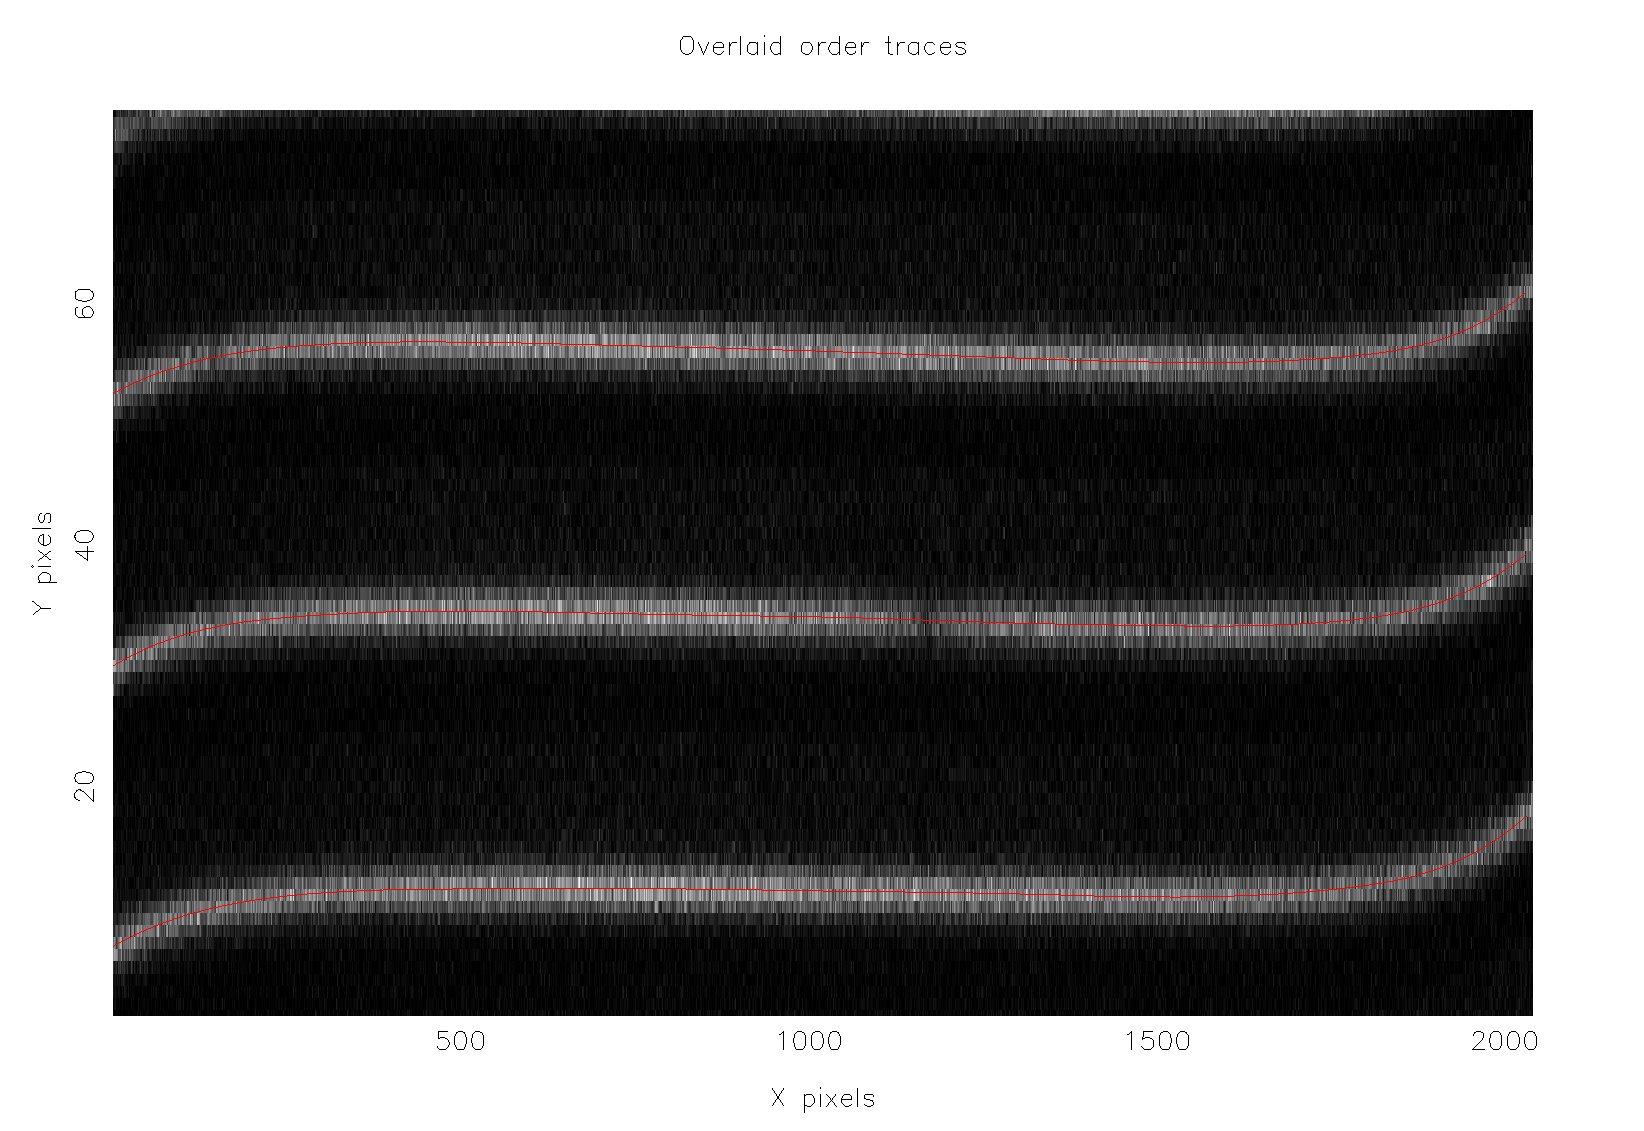
\includegraphics[height=60mm]{sun152_cover}}
% ? End of document identification
% -----------------------------------------------------------------------------
% ? Document specific \providecommand or \newenvironment commands.

\providecommand{\mlabel}[1]{\xlabel{#1}\label{#1}}

\setcounter{tocdepth}{2}
\setcounter{secnumdepth}{3}
\renewcommand{\floatpagefraction}{0.8}

%begin{latexonly}
% To generate the index, invoke as
%     latex '\def\generateindex{1}\input sun152'
\providecommand{\generateindex}{0}
\ifcase\generateindex
  \typeout{Not generating index}
\else
  \typeout{Generating index}
  %\usepackage{makeidx}	% unnecessary, since we incorporate the
				% generated index completely, at the bottom
  \makeindex
\fi


\providecommand{\sunspec}[2]{#1}

% \cmdname{blah_blah} formats command names, and accepts underscores
\providecommand{\cmdname}{\begingroup \catcode`\_=12 \realcmdname}
\providecommand{\realcmdname}[1]{\endgroup\texttt{#1}}

\providecommand{\myindex}[1]{\index{#1}}
\providecommand{\indexcmdname}[1]{\index{#1@\protect\cmdname{#1}}}

\providecommand{\echtask}[4]{
   \goodbreak
   \rule{\textwidth}{0.5mm}
   \vspace{-7ex}
   \newline
   \settowidth{\sstbannerlength}{{\Large {\bf #3}}}
   \setlength{\sstcaptionlength}{\textwidth}
   \addtolength{\sstbannerlength}{0.5em}
   \addtolength{\sstcaptionlength}{-2.0\sstbannerlength}
   \addtolength{\sstcaptionlength}{-5.0pt}
   \parbox[t]{\sstbannerlength}{\flushleft{\Large {\bf #3}}}
   \parbox[t]{\sstcaptionlength}{\center{\Large #4}}
   \parbox[t]{\sstbannerlength}{\flushright{\Large {\bf #3}}}
   \label{#1}\label{#2}
   \uppercase{\myindex{#2@\protect\cmdname{#2}}}
}

\providecommand{\echparameter}[4]
{
\item [#1 = #3] \mbox{}\label{par_#2}\indexcmdname{#2}\\
#4
}

\providecommand{\echpars}[1]{
{\bf Parameters:\vspace*{6pt}\\}
    #1
}

\providecommand{\epar}[3]
{
    \hspace*{5mm}\makebox[50mm][l]{\bf #1} #2 (p~\pageref{par_#3}.)\\
}

\providecommand{\lepar}[3]
{
    \hspace*{5mm}\makebox[50mm][l]{\bf #1} #2 (p~\pageref{par_#3}.)
}

\providecommand{\echredobj}[1]{
{\bf Reduction File Objects:\vspace*{6pt}\\}
      \hspace*{5mm}\makebox[50mm][l]{Object}\makebox[25mm][l]{Type}{Access}\\
      #1
}

\providecommand{\eobj}[3]
{
    \hspace*{5mm}\makebox[50mm][l]{\bf #1}\makebox[25mm][l]{\tt #2}{\tt #3}\\
}

\providecommand{\leobj}[3]
{
    \hspace*{5mm}\makebox[50mm][l]{\bf #1}\makebox[25mm][l]{\tt #2}{\tt #3}
}

%end{latexonly}

% HTML versions
\begin{htmlonly}
\providecommand{\sunspec}[2]{#2}

\providecommand{\cmdname}[1]{#1}
\providecommand{\myindex}[1]{}
\providecommand{\indexcmdname}[1]{}

\providecommand{\echtask}[4]
{
  \subsection{\xlabel{#1}\xlabel{#2}\label{#1}\label{#2}#3---#4}
}

\providecommand{\echparameter}[4]
{
  \subsection{\xlabel{par_#2}\label{par_#2}{\bf #1}}
  {\bf Type: #3}\\
#4
}

\providecommand{\echpars}[1]{
{\bf Parameters:}
\begin{itemize}
#1
\end{itemize}
}

\providecommand{\epar}[3]
{\item \htmlref{{\bf #1}}{par_#3} - #2}

\providecommand{\lepar}[3]
{\item \htmlref{{\bf #1}}{par_#3} - #2}

\providecommand{\echredobj}[1]{
{\bf Reduction File Objects:}
\begin{itemize}
#1
\end{itemize}
}

\providecommand{\eobj}[3]
{\item {\bf #1} - {\it type:} #2, {\it access:} #3.}

\providecommand{\leobj}[3]
{\item {\bf #1} - {\it type:} #2, {\it access:} #3.}
\end{htmlonly}

% star2HTML and post-processing
% =============================
%
% This following can be used to invoke star2html and post-process this
% document to generate HTML as the author intended.
%
% To run the script, automatically extracting from this file:
%
%    sed -n 's/^%%S2HPOST//p' sun152.tex | sh

%%S2HPOST#!/bin/sh
%%S2HPOST
%%S2HPOST# Definitions.
%%S2HPOST    #set AUTH_NAME = 'Martin Clayton';
%%S2HPOST    #set AUTH_EMAIL = 'mjc@star.ucl.ac.uk';
%%S2HPOST    AUTH_NAME='Norman Gray';
%%S2HPOST    AUTH_EMAIL='norman@astro.gla.ac.uk';
%%S2HPOST    DOC_CODE=sun152;
%%S2HPOST    DOC_TITLE='ECHOMOP-Echelle Data Reduction Package';
%%S2HPOST
%%S2HPOST# Star2html process.
%%S2HPOST    if test -f sun152.aux; then
%%S2HPOST        useaux=-aux
%%S2HPOST    else
%%S2HPOST        useaux=
%%S2HPOST    fi
%%S2HPOST    ${STAR2HTML:=star2html} -a "${AUTH_NAME}" -m "${AUTH_EMAIL}" $useaux \
%%S2HPOST            -t "${DOC_TITLE}" ${DOC_CODE}
%%S2HPOST
%%S2HPOST# Generate Perl script to do the work.
%%S2HPOST    cat > ${DOC_CODE}$$.pl <<FOO
%%S2HPOST#!/usr/bin/perl
%%S2HPOST
%%S2HPOST# To be used in a pipe.
%%S2HPOST# Post-processing for star2html.
%%S2HPOST
%%S2HPOST\$last_line = '';
%%S2HPOST\$last_invisanchor = 0;
%%S2HPOST\$AUTH_EMAIL = '$AUTH_EMAIL';
%%S2HPOST
%%S2HPOST\$nlines = 0;
%%S2HPOSTwhile ( <> ) {
%%S2HPOST
%%S2HPOST# Add mailto URL if e-mail address is found.
%%S2HPOST    s#\$AUTH_EMAIL#<A HREF="mailto:\${AUTH_EMAIL}">\${AUTH_EMAIL}</A>#;
%%S2HPOST
%%S2HPOST# Some small adjustments - gets rid of blank space at page top.
%%S2HPOST    s/<P><ADDRESS>/<ADDRESS>/;
%%S2HPOST    s/<BR> <HR>/<HR>/g;
%%S2HPOST    s/<HR> <P>/<HR>/g;
%%S2HPOST    s/<DD>  <BR>/<DD>/g;
%%S2HPOST
%%S2HPOST# Correct problem with ~ being missed in some of my URLs.
%%S2HPOST#    s-ucl.ac.uk/ mjc-ucl.ac.uk/~mjc-;
%%S2HPOST
%%S2HPOST# Convert em dashes into single hyphens.
%%S2HPOST    s/([^-])---([^-])/\1-\2/g;
%%S2HPOST
%%S2HPOST# Try to get rid of "invisible" anchors by tying them to the next word.
%%S2HPOST# Also try to handle "doubles" caused by \xlabel{}\label{} type things.
%%S2HPOST    s:(<H[1-9]><A NAME=SECTION[^>]*><A NAME=[^>]*>)&#160;(</A>)(<A NAME=[^>]*>)&#160;(</A>)([^<]*):\1\3\5\2\4:;
%%S2HPOST    s:(<H[1-9]><A NAME=SECTION[^>]*><A NAME=[^>]*>)&#160;(</A>)([^<]*):\1\3\2:;
%%S2HPOST
%%S2HPOST# Same procedure for invisible anchors in list items...
%%S2HPOST    s:(<LI> <b><A NAME=[^>]*>)&#160(</A>)([^<]*)(</b><BR>):\1\3\2\4:;
%%S2HPOST
%%S2HPOST# Minor correct for some lists.
%%S2HPOST    s:<LI> :<LI>:;
%%S2HPOST
%%S2HPOST# Get rid of double horizontal rules (shouldn't be any...)
%%S2HPOST    if ( \$last_line eq "<HR>\n" ) {
%%S2HPOST        if ( \$_ eq "<HR>\n" ) {
%%S2HPOST            next;
%%S2HPOST        }
%%S2HPOST
%%S2HPOST# Get rid of double Paragraph breaks.
%%S2HPOST    } elsif ( \$last_line eq "<P>\n" ) {
%%S2HPOST        if ( \$_ eq "<P>\n" ) {
%%S2HPOST            next;
%%S2HPOST        }
%%S2HPOST
%%S2HPOST# This is an attempt to convert invisible anchors introduced by \indexentry
%%S2HPOST# to be attached to the next word.
%%S2HPOST    } elsif ( \$last_invisanchor != 0 ) {
%%S2HPOST        if ( \$_ eq "<P>\n" ) {
%%S2HPOST            next;
%%S2HPOST
%%S2HPOST        } else {
%%S2HPOST            \$last_invisanchor = 0;
%%S2HPOST            ( \$firstword, \$rest ) = split( ' ', \$_, 2 );
%%S2HPOST            print "\$1\$firstword\$2 \$rest";
%%S2HPOST            \$last_line = \$_;
%%S2HPOST            next;
%%S2HPOST        }
%%S2HPOST    }
%%S2HPOST
%%S2HPOST# Note that an \indexentry introduced anchor is here.
%%S2HPOST    if ( m-^[ ]?(<A NAME=[^>]*>)&#160;(</A>)- ) {
%%S2HPOST        \$last_invisanchor = 1;
%%S2HPOST        \$last_line = \$_;
%%S2HPOST        next;
%%S2HPOST
%%S2HPOST    }
%%S2HPOST
%%S2HPOST    print;
%%S2HPOST    \$last_line = \$_;
%%S2HPOST
%%S2HPOST# Encapsulate page in HTML tags.
%%S2HPOST    if ( \$nlines == 0 ) {
%%S2HPOST       print "<HTML>\n";
%%S2HPOST       \$nlines = 1;
%%S2HPOST    }
%%S2HPOST}
%%S2HPOST
%%S2HPOST# End encapsulate
%%S2HPOSTprint "</HTML>\n";
%%S2HPOST
%%S2HPOST#
%%S2HPOST# End-of-file.
%%S2HPOSTFOO
%%S2HPOST    chmod 755 ${DOC_CODE}$$.pl
%%S2HPOST
%%S2HPOST# Make changes.
%%S2HPOST    cd ${DOC_CODE}.htx
%%S2HPOST    echo ''
%%S2HPOST    echo "! star2html post-processing ${DOC_CODE}."
%%S2HPOST    echo -n "! General HTML changes"
%%S2HPOST    for f in *.html; do
%%S2HPOST        ../${DOC_CODE}$$.pl <$f > temp$$.html
%%S2HPOST        mv -f temp$$.html $f
%%S2HPOST        echo -n '.'
%%S2HPOST    done
%%S2HPOST    rm -f ../${DOC_CODE}$$.pl
%%S2HPOST    rm -f temp$$.html
%%S2HPOST    echo ''
%%S2HPOST
%%S2HPOST# Hyperlink so that links in the document should work.
%%S2HPOST    echo '! Hyperlinking document against Master Document Set at RAL.'
%%S2HPOST    cd ..
%%S2HPOST    HTX_PATH=.; export HTX_PATH
%%S2HPOST    ${HLINK:=hlink} .
%%S2HPOST    echo '! Hyperlink done.'
%%S2HPOST    echo '! star2html post-processing complete.'
%%S2HPOST
%%S2HPOSTexit

% ? End of document specific commands
% -----------------------------------------------------------------------------
%  Title Page.
%  ===========
\begin{document}
\scfrontmatter

% ? Main text
%%%%%%%%%%%%%%%%%%%%%%%%%%%%%%%%%%%%%%%%%%%%%%%%%%%%%%%%%%%%%%%%%%%%%%%%%%%
\section{\mlabel{introduction}INTRODUCTION}

{\sc echomop} provides a set of tasks to expedite the reduction of \'{e}chelle
spectra data frames.  The options available range from full-scale
automated reduction to step-by-step, order-by-order manually-assisted
processing.  The tasks were written originally for the reduction of
data from the University College London Echelle Spectrograph (UCLES);
however, the algorithms are sufficiently flexible to permit reduction of
spectra from a wide variety of sources.


\subsection{\mlabel{facilities}Summary of Facilities}

Below is a brief summary of what can be done with {\sc echomop}.
It should help you to decide whether {\sc echomop} can help you with your
data reduction.

\begin{itemize}

\item Spectral order location.
\item Cosmic-ray removal.
\item Detection of bad image rows and columns, and saturated pixels.
\item Spectral order tracing.
\item Determination of object channels.
\item Generation of flat-field balance models.
\item Modelling of scattered light.
\item Optimal spectrum extraction.
\item Echelle blaze correction.
\item Quick-look spectral extraction.
\item Automated location of lines in arc spectra.
\item Wavelength calibration of arc spectra.
\item Distortion fitting for spectral orders.
\item Extraction of distorted orders.
\item Scrunching of extracted spectral orders.
\item Production of distortion-free image.
\item Plotting of data used for a reduction.
\item Output of products.

\end{itemize}

All {\sc echomop} facilities can be accessed from a single task, ECHMENU,
which guides you through a reduction.


\subsection{ How to Use this Document}

There is an \xref{{\sl Introduction to Echelle Spectroscopy} (SG/9)}{sg9}{}
which is a good starting point for those new to \'{e}chelle data reduction.

If you are new to {\sc echomop}, you should refer to the demonstration
described in the next sub-section and become familiar with the basic
steps used to perform a reduction in
\sunspec{\S\ref{standard_steps}}{\htmlref{Standard
Steps}{standard_steps}}\@.
It is a good idea to read
\sunspec{Appendix~\ref{notes_for_observers}}{the \htmlref{Notes for
Observers}{notes_for_observers}} prior to observing.

More experienced users will want to refer to the detailed task and parameter
information
\sunspec{in \S\ref{tasks_options}}{under \htmlref{Tasks}{tasks_options}}
and \sunspec{\S\ref{parameters}}{\htmlref{Parameters}{parameters}}\@.

The remainder of this document contains the following information:

\sunspec{\S\ref{using_echomop}}{\htmlref{Using
{\sc echomop}}{using_echomop}} describes the basic use of the main
{\sc echomop} task ECHMENU and the single-option tasks available from the shell.

\sunspec{\S\ref{tasks_options}}{\htmlref{Tasks \&
Options}{tasks_options}} gives more detailed information on each task
with lists of all the parameters used by each task.

\sunspec{\S\ref{parameters}}{\htmlref{Parameters}{parameters}}
describes all {\sc echomop} parameters in full.

\sunspec{\S\ref{automatic_reductions} and \S\ref{cloning}}{
\htmlref{Automatic Reductions}{automatic_reductions} and
\htmlref{Cloning}{cloning}} briefly
outline the important considerations for reducing multiple datasets
automatically using a `template' reduction performed manually.

\sunspec{\S\ref{tips}}{The \htmlref{Tips}{tips} section}
provides advice on handling particular types of data and specific processing
techniques.

\sunspec{\S\ref{input_files} and \S\ref{output_files}}{The
sections on
\htmlref{Input Data}{input_data} and \htmlref{Output Data}{output_data}}
describe {\sc echomop} input and output data formats.

\sunspec{\S\ref{echarc_imp_exp}}{\htmlref{ECHARC}{echarc_imp_exp}}
describes the inter-operability of
{\sc echomop} with the \xref{{\sc figaro}}{sun86}{} \xref{ECHARC}{sun86}{ECHARC} program.

\sunspec{Appendix~\ref{notes_for_observers}}{The \htmlref{Notes for
Observers}{notes_for_observers}} gives advice on how to go about
preparing for an \'{e}chelle observing run and what needs to be done
with your data prior to using {\sc echomop} for the spectral extraction.

\sunspec{Appendix~\ref{hints} is}
{The \htmlref{Hints}{hints} are}
based on information in the on-line HELP text.
Each sub-section describes the cause of an {\sc echomop} problem and offers
possible solutions.

\sunspec{Appendix~\ref{release_notes} is}
{The \htmlref{Release Notes}{release_notes} are} the change log for
{\sc echomop}.  Information about the current release is included.

\subsection{\mlabel{demonstration}Demonstration}

You can obtain an on-line introduction to the use of {\sc echomop},
after you have setup {\sc echomop} as described in
section~\ref{getting_started}, by typing the command

\begin{terminalv}
% ech_demo -graphics-device-
\end{terminalv}

where {\tt -graphics-device-} is available for plotting the graphs
during the reduction ({\it{e.g.,}} \texttt{xw}). \myindex{Demonstration}
This runs a demonstration reduction using a set of example data
frames.  It demonstrates the main functions of {\sc echomop} and follows
a simple reduction from the start to the production of an extracted,
wavelength-calibrated spectrum.  The text of the demonstration is also
available for printing in the file

\begin{terminalv}
$ECHOMOP_DEMO/ech_demo.txt
\end{terminalv}
%$% dollar matching hack
for those who prefer to read from a paper copy whilst running the demo.


%%%%%%%%%%%%%%%%%%%%%%%%%%%%%%%%%%%%%%%%%%%%%%%%%%%%%%%%%%%%%%%%%%%%%%%%%%%
\section{\mlabel{using_echomop}USING ECHOMOP}
\myindex{Starting up}

{\sc echomop} may be used in a variety of ways depending upon your expertise.

The most convenient method for normal use is to start the main ECHMENU
task.
This task provides a guided path through the processes of a\sunspec{
`standard reduction' (see \S\ref{standard_steps})}{\htmlref{standard
reduction}{standard_steps}}.

\subsection{\mlabel{getting_started}Getting Started}
\myindex{Monolith}

{\sc echomop} is prepared for use from the shell by typing the command:

\begin{terminalv}
% echomop
\end{terminalv}

To start a reduction type:

\begin{terminalv}
% echmenu
\end{terminalv}

at the command-line prompt.

{\sc echomop} uses a disc-based `reduction database' to store objects which may need
to be passed between various reduction tasks.\myindex{Reduction database}
You will initially be asked to provide a name for this file, which will then
be created in the current directory.
This file is associated with a particular set of data frames
(object, arc, flat {\it etc.}) thereby providing the ability to
replay any aspect of the reduction at a later date.
Reduction files can occupy a large amount of disk space and you may wish to
delete them once the reduced spectrum has been obtained.

When running, ECHMENU will provide a default for the next task to be
performed; this will usually be the correct one for a standard reduction.
To accept the recommended next step, it is only necessary to press one of the
accept characters followed by a carriage return.  Recognised accept characters
are `Y', `+', and `/'. \myindex{Accept character}

\subsection{\mlabel{ECHMENU}ECHMENU}

The simplest method of using {\sc echomop} is via the task ECHMENU which has
access to all the processing modules, along with a set of utilities for
interactive tuning of parameters, and plotting of graphs of intermediate
results.  As a reduction progresses, the details and results of each task
are stored in a disk file allowing the repetition or alteration of any aspect
of the reduction at any stage. \myindex{Reduction database} ECHMENU
prompts for the name of this `reduction database' file when it
starts.  If the name of an existing reduction-database is given then
this file will be opened, otherwise the package will create a new file
using the name provided.  The name of the file may also be provided on the
command line, {\it{e.g.}}:

\begin{terminalv}
% echmenu ech_rdctn=filename
\end{terminalv}

Once the reduction-database has been opened, the main menu is
presented.  This menu consists of all the major steps in the reduction
process, along with a set of utility options, and some more specialised
options ({\it{e.g.}}, 2-D distortion correction). \myindex{Option!selection
of}  An option is selected by typing its number followed by carriage
return.  Some options may also be selected by entering a keyword (or its
first character) followed by carriage return, {\it{e.g.}},

\begin{terminalv}
PLOT
\end{terminalv}

or

\begin{terminalv}
P
\end{terminalv}

would select the graph plotting utility.  Some options consist of sets of
different tasks which usually need to be run together.  It is possible to
run these sub-options individually by typing the number and sub-option
number in the form main.sub-option  ({\it{e.g.}}, 1.2).
\myindex{Sub-options!selection of} {\sc echomop} attempts to provide the most
sensible option (for a standard reduction) as the default, and you
can accept this simply by typing one of the accept characters ({\it{e.g.}},
`Y'), plus a carriage return. \myindex{Help} Option 0 always
provides HELP information on the default option, and then allows you
to browse the HELP library for more detailed information.

Most options invoke processing modules.  These modules will usually
require the specification of a number of parameters which will be
automatically prompted for by the program.  It is possible to
preview/edit all the parameters (including any hidden ones) for any
option by entering its number prefixed by a minus sign. {\it{e.g.}},
-3 would allow preview/edit of the parameters used by option 3.
\myindex{Prompt}

\begin{quote}

  {\bf NOTE:} {\sl In general, once a parameter has been provided
  it will NOT be re-prompted for by any module which requires it.
  The modules will simply re-use the value already supplied. The -option
  strategy overrides this behaviour and allows you to change any
  parameter value at any point.}

\end{quote}

Any parameter can be provided on the startup command-line, in
this case the parameter will not be prompted for.


\subsection{\mlabel{graphic_display}Graphic Display}
\myindex{Graphics!setting device}

Graphics display is controlled by the parameter:

\begin{terminalv}
soft=/device/
\end{terminalv}

The \xref{{\sc figaro}}{sun86}{} \xref{SOFT}{sun86}{SOFT} command

\myindex{FIGARO!SOFT}
\begin{terminalv}
% soft options
\end{terminalv}

may be used to get a list of available graphics devices.

\myindex{Graphics!null device}
{\sc echomop} also supports both \texttt{SOFT=NONE} and \texttt{SOFT=NULL}
which disable all interactive graphics facilities and save CPU time when
such facilities are not required.

\myindex{Graphics!hardcopy}
Hardcopy graphics is directed to {\tt /device/} using the parameter:

\begin{terminalv}
hard=/device/
\end{terminalv}

and enabled (in preference to on-screen graphics) using the hidden
parameter \texttt{HARDCOPY} when starting {\sc echomop} tasks, {\it{e.g.}}:

\begin{terminalv}
% echmenu hardcopy=y /any-other-parameters/
\end{terminalv}


\subsection{\mlabel{image_display}Image Display}
\myindex{Image display}

Before proceeding with a reduction it is recommended that the data frame
be examined on an imaging display to ensure that the orders are
orientated as {\sc echomop} expects (See \sunspec{\S\ref{orientation}}
{\htmlref{Orientation of Spectra}{orientation}}).

If an imaging graphics display is available then you can use the
DISPLAY command-line parameter when invoking {\sc echomop} tasks, {\em e.g}:

\begin{terminalv}
% echmenu display=yes /other-parameters/
\end{terminalv}

The image display will automatically be used to:
\myindex{Image display!use by monolith}

\begin{itemize}
\item {over-plot order trace paths in Options 2 and 15.}
\item {over-plot extracted object limits in Option 19.}
\item {determine positions for `browse' option in the plotter.}
\end{itemize}


\subsection{\mlabel{parameters_prompts}Parameters and Prompts}
\myindex{Parameters}

Most of the user-input information required by {\sc echomop} is obtained
using the \xref{ADAM parameter system}{sg4}{}.
This standard method for getting values leads to a consistency of
user-interface between all \xref{ADAM}{sg4}{}-based tasks.
However, in some cases it is more convenient to present the user with a menu
and this approach is used for the top-level selection of processing steps,
and also during interactive graphic steps.
\myindex{ADAM!parameters}
When an ADAM parameter is prompted for, the default value (used if the
response is carriage-return only) is indicated enclosed in single quotes and
back slashes ({\tt /' '/}).
Instead of entering a value you may also use the following special
responses which are processed by the ADAM parameter system:

\begin{itemize}

\item [\texttt{?}] --- provides information on parameter type, minimum and
      maximum allowed values {\it etc.}

\item [\texttt{??}] ---  provides same information as above and then allows
      you to browse the HELP library.

\item [\texttt{!!}] --- \myindex{Abort!option}\myindex{Option!abort}
      requests an abort of the task.

\item [\sunspec{$\backslash$}{\texttt{\backslash}}] ---
      \myindex{Prompt!disabling} causes all
      subsequent parameters to adopt their default values {\bf without}
      further prompts. (May also be appended to a value response, {\it
      {e.g.}}, \verb+10\+ would set the current parameter to 10 and
      switch off any further prompting).

\end{itemize}

\subsection{\mlabel{tuning_parameters}Tuning Parameters}
\myindex{Parameters!tuning}

{\sc echomop} tasks use a number of `hidden'
parameters.\myindex{Parameters!hidden}
These will not normally need to be changed, but provide flexibility when
processing problem data.  They are also used by ECHMENU to configure itself
for `quick-look' extraction. \indexcmdname{ECH_TUNER}
ECHMENU Option~23 allows you to interactively examine and alter these
parameters.  Parameter values may also be supplied on task command-lines.
{\sc echomop} tasks always report any \verb+TUNE_+ parameters which have
been set to non-default values.


\subsection{\mlabel{processing_steps}Processing Steps}

The reduction cycle has been split into a set of steps, most of which
perform some form of image analysis.  The results of these analysis steps
provide various function fits and data  describing the features of the
image. All these steps take place before any extraction of data from the
raw image. The extraction is performed in a single step taking into account
the previously established data characteristics. This provides for the
efficient processing of multiple data frames\myindex{Multiple data frames}
where the same object has been observed, as many of the processing steps
need only be done once, for the first frame of the series.

All the discrete processing steps are available as both individual tasks
(providing efficient execution of single steps), and as options from a
menu-driven control task (providing automatic processing and context-sensitive
assistance).

To run a particular step you can:

\begin{itemize}

\item select the appropriate option from the main ECHMENU menu.

\item type the task name at the command line, {\it{e.g.}}:

\begin{terminalv}
% ech_linloc
\end{terminalv}

\end{itemize}

\begin{quote}

   {\bf NOTE:} {\sl that when using the individual tasks the strategy for
   selecting single order/all order operation is different.  Individual
   tasks which can operate on single orders all utilise the parameter:

\begin{terminalv}
IDX_NUM_ORDERS
\end{terminalv}

   with which you should specify the number of the order to process, or a
   zero to indicate that all orders are to be processed in turn.}
\end{quote}


\subsection{\mlabel{repeating_steps}Repeating Steps}
\myindex{Repeating steps}

In many cases the automatic sequence of steps provided by the ECHMENU
main menu defaults will be enough to complete the reduction. In some
cases however, it may be necessary to restart the reduction at a
particular stage, maybe using a different raw image, different degree
of polynomial {\it etc}.

ECHMENU allows the selection of any valid step of a reduction at any stage.
If the step requested needs results from steps which have not yet been
performed then you will be informed of this and the default next step
will be set back to the step which generates the required information.
\myindex{Single step tasks}
If a single step task is invoked before all its input requirements are
available ({\it{e.g.}}, order tracing before order location) then the task
will abort with a message indicating which task needs to be run in order to
provide the necessary pre-requisites.


\subsection{\mlabel{standard_steps}Standard Steps}

The following steps constitute a standard reduction as implemented by
the monolithic ECHMENU task.  You can follow this sequence by hitting
Y and carriage-return at each main menu prompt, and supplying data frame names
and parameters values when prompted.
\myindex{Frame!dimensions}
\myindex{Cosmic rays}
\myindex{Order!slope}
\myindex{Slope of orders}
\myindex{Order!location}
\myindex{Locating orders}

\begin{itemize}

\item 1 --- Start a reduction (\verb+ech_locate+).

\begin{itemize}

   \item 1.1 --- Check frame dimensions
         (\htmlref{{\tt{ech\_fcheck}}}{ech_fcheck}).

   \item {1.2 --- Check trace frame for cosmic-ray hits/bad rows and columns
         (\htmlref{{\tt{ech\_decos1}}}{ech_decos1}).}

   \item {1.3 --- Determine order slope
         (\htmlref{{\tt{ech\_slope}}}{ech_slope}).}

   \item {1.4 --- Count orders
         (\htmlref{{\tt{ech\_count}}}{ech_count}).}

   \item {1.5 --- Locate orders
         (\htmlref{{\tt{ech\_locate}}}{ech_locate}).}

\end{itemize}

\item {2 --- Trace the orders and fit polynomials
      (\htmlref{{\tt{ech\_trace}}}{ech_trace}).}
\myindex{Order!tracing}
\myindex{Trace!orders}

\item {3 --- Clip trace polynomial fits
      (\htmlref{{\tt{ech\_fitord}}}{ech_fitord}).}
\myindex{Dekker limits}
\myindex{Object limits}
\myindex{Extraction limits}

\item {4 --- Determine dekker limits and sky/object channels
      (\htmlref{{\tt{ech\_spatial}}}{ech_spatial}).}

\begin{itemize}
\item {4.1 --- Determine dekker limits
      (\htmlref{{\tt{ech\_dekker}}}{ech_dekker}).}

\item {4.2 --- Determine object and sky channels
      (\htmlref{{\tt{ech\_object}}}{ech_object}).}

\end{itemize}

\myindex{Flat field}
\item {5 --- Model flat-field per-pixel balance factors
      (\htmlref{{\tt{ech\_ffield}}}{ech_ffield}).}

\myindex{Sky!model}
\item {6 \sunspec{---}{-} Model sky background
      (\htmlref{{\tt{ech\_sky}}}{ech_sky}).}

\myindex{Object!profile}
\myindex{Profile!object}
\item {7 --- Model object profile
      (\htmlref{{\tt{ech\_profile}}}{ech_profile}).}

\myindex{Extraction}
\item {8 --- Extract object and arc spectra
      (\htmlref{{\tt{ech\_extrct}}}{ech_extrct}).}

\myindex{Arc line!location}
\myindex{Arc line!FWHM}
\item {9 --- Locate arc lines and fit Gaussian profiles
      (\htmlref{{\tt{ech\_linloc}}}{ech_linloc}).}

\begin{itemize}

   \item {9.1 --- Determine average arc line FWHM
         (\htmlref{{\tt{ech\_fwhm}}}{ech_fwhm}).}

   \item {9.2 --- Locate arc line candidates
         (\htmlref{{\tt{ech\_lines}}}{ech_lines}).}

\end{itemize}

\myindex{Wavelength calibration}
\myindex{Arc line!calibration}
\item {10 --- Identify arc lines and fit wavelength scales
      (\htmlref{{\tt{ech\_idwave}}}{ech_idwave}).}

\item {11 --- Model blaze profile and apply to object spectrum
      (\htmlref{{\tt{ech\_blaze}}}{ech_blaze}).}

\myindex{Order!ripple}
\begin {itemize}

   \item {11.1 --- Model order ripple
         (\htmlref{{\tt{ech\_fitblz}}}{ech_fitblz}).}

   \item {11.2 --- Correct order ripple
         (\htmlref{{\tt{ech\_doblz}}}{ech_doblz}).}

\end{itemize}

\item {12 --- Scrunch object spectrum
      (\htmlref{{\tt{ech\_scrunch}}}{ech_scrunch}).}

\begin{itemize}

   \item {12.1 --- Fit arc-line FWHMs as a function of wavelength
         (\htmlref{{\tt{ech\_fitfwhm}}}{ech_fitfwhm}).}

   \item {12.2 --- Calculate wavelength scale
         (\htmlref{{\tt{ech\_wscale}}}{ech_fit_wscale}).}

   \myindex{Scrunch!object}
   \item {12.3 --- Scrunch extracted object orders
         (\htmlref{{\tt{ech\_scrobj}}}{ech_scrobj}).}

   \myindex{Scrunch!arc}
   \myindex{Arc line!FWHM fit}
   \item {12.4 --- Scrunch extracted arc orders
         (\htmlref{{\tt{ech\_scrarc}}}{ech_scrarc}).}

\end{itemize}

\item {14 --- Write results file
      (\htmlref{{\tt{ech\_result}}}{ech_result}).}

\end{itemize}

\myindex{Output}
\myindex{Results}
\myindex{Demonstration}

The demonstration provided by \verb+ech_demo+ follows this overall sequence
and the reader is encouraged to try it before using {\sc echomop} in earnest.
\myindex{Wavelength calibration!none} Steps 9 through 12 would be omitted if
no wavelength calibration\myindex{Arc calibration!none} was required.
Step 5 would be omitted if no flat field was
available. \myindex{Multiple object frames}  In cases where multiple object
frames have been taken, it would be efficient to use only steps 6, 7, 8, 11,
12 for additional frames.\myindex{Quick-look extraction}
\myindex{Extraction!quick-look}  A quick-look extraction may be performed as
soon as step 4 has been completed (using Option~19).


\subsection{\mlabel{sub-options}Accessing Single Function Sub-options}
\myindex{Sub-options}

Many of the ECHMENU main menu tasks consist of a number of independent
functions which are automatically invoked. For example Option 12 consists
of 4 sub-options. The ECHMENU program allows the selection of any sub-option
directly, {\it{e.g.}}:

\begin{terminalv}
12.3
\end{terminalv}

would select Option~12.3 (Scrunch extracted object order) explicitly.

To check if sub-options are available, the context specific HELP for the
option should be viewed (type 0 at the main menu prompt). Some
sub-options are individually accessible when using the single purpose
tasks ({\it{e.g.}}, \texttt{ech\_scrarc}).


\subsection{\mlabel{automation}Automation}
\myindex{Automation}

{\sc echomop} provides automation to many aspects of \'{e}chelle data reduction
which have traditionally required substantial interactive assistance:

\myindex{Automation!functions}
\begin{itemize}

\item Order location
\item Cosmic-ray pixel identification
\item Object/Sky pixel classification
\item Arc line identification

\end{itemize}

The provision of these features permits the completely automatic
reduction of \'{e}chelle data frames.  To help ensure the success of
automatic reduction runs, special attention should be made to ensure
that the following conditions are satisfied:

\myindex{Automation!requirements}
\begin{itemize}

\item A bright continuous spectrum image is provided for order
      tracing.

\item The trace/arc/object images supplied are the correct ones. For
      instance supplying the wrong arc image will cause problems if the
      orders are in different places on the detector.

\item Constraints placed on the expected range of wavelength and
      dispersion are wide enough. {\it{e.g.}}, if in doubt about the
      dispersion being 0.2 or 0.3 Angstroms per-pixel, provide limits of
      \htmlref{{\tt MIN\_DISPERSION=0.1}}{par_MIN_DISPERSION},
      \htmlref{{\tt MAX\_DISPERSION=0.5}}{par_MAX_DISPERSION}.

\end{itemize}


\subsection{\mlabel{quick_look_mode}Quick-look Mode}
\myindex{Quick-look mode}

Invoking ECHMENU with the \htmlref{{\tt TUNE\_QUICK=Y}}{par_TUNE_QUICK}
will cause the automatic setting of tuning parameters to values designed for
fastest processing.

The following algorithmic optimizations will be used:
\indexcmdname{TUNE_QUICK}

\begin{itemize}

\item order tracing will use centre-of-gravity to locate the centre
      of the order.

\item a maximum of 200 trace sample points per order will be measured.

\item criteria for clipping points from the trace fit will be set
      at 1-pixel maximum deviation, and up to 5 pixels may be clipped
      per iteration.

\item extraction will use the simple version of the 1-D algorithm
      which is faster than optimal/weighted extraction.

\item arc-line identification will assume the data is arranged
      with wavelength increasing with X-pixel number.

\end{itemize}


\subsection{\mlabel{error_arrays}Error Arrays}
\myindex{Errors!arrays}
\myindex{Variance}

{\sc echomop} can deal with errors from the following variety of sources:

\myindex{Flat field!errors}

\begin{itemize}

\item Errors on the flat-field frame which should be provided in the
      flat-field frame error array.  If no error array is provided then
      estimates using root-n statistics are used.

\myindex{Readout noise}
\item Errors due to the readout-noise on CCD type detectors. The
      readout noise value is supplied as a parameter and is applied to the
      whole frame when calculating the variances on extracted pixels.

\myindex{Errors!additive}
\item Linear error sources determined may be treated by
      providing an error array associated with the object data frame. The
      values should represent an error source that does not vary with the
      intensity of the particular pixel involved. An example of this type
      of error source would be the bias subtraction. If many bias frames
      are available, then the error  for each detector pixel can be
      determined.
      Supplying these errors as the object error array
      would then cause them to be correctly included in the variance
      calculations during extraction.

\myindex{Errors!multiplicative}
\item Multiplicative errors such as those due to errors on the balance
      factors (from the flat field) may be taken into account by
      incorporating the appropriate values in the error array supplied with
      the flat-field frame. It is up to you to ensure these variances
      correctly represent the combined effect of both the flat-field noise
      and any additional multiplicative error source(s).

\myindex{Sky!errors}
\myindex{Errors!Sky model}
\item Errors due to sky modelling and subtraction are calculated and
      processed internally by the extraction task.

\myindex{Errors!due to cosmic rays}
\item Errors due to detected cosmic-ray hits are treated by ignoring the
      contaminated pixel and rescaling the variance on the remaining pixels
      in that (wavelength) increment.

\myindex{Errors!output}
\item All output spectra have an error array associated with them, these
      error arrays always contain the variance for the parallel entry in
      the data arrays.

\end{itemize}


%%%%%%%%%%%%%%%%%%%%%%%%%%%%%%%%%%%%%%%%%%%%%%%%%%%%%%%%%%%%%%%%%%%%%%%%%%%
\section{\mlabel{tasks_options}ECHOMOP TASKS \& ECHMENU OPTIONS}
\mlabel{echomop_options}
\myindex{Standard reduction!sequence}
\myindex{Main menu!monolith}

The ECHMENU monolith main menu options are described in the following text.
Many of these options are also available as tasks which can be
accessed from the shell.  Where a task is available its name is given in the
section heading.

In each of the following sections a description is given of the task, it's
purpose, the parameters it uses and the reduction file objects it accesses.
Parameters used by the tasks are described in detail
\sunspec{in \S\ref{parameters}}{under \htmlref{Parameters}{parameters}}\@.


\echtask{option0}{echhelp}{0:{\tt echhelp}}{HELP}
\myindex{Help}

Provides entry into the HELP library for browsing. Upon entry the first
topic displayed will depend upon the context and will usually be
appropriate to the next default option at the time.

To leave the HELP type a CTRL-Z, or hit carriage-return until the
ECHMENU menu re-appears.

The stand-alone HELP browser \texttt{echhelp} can be invoked from the shell
or the hypertext version of the text can be accessed using

\begin{terminalv}
% echwww
\end{terminalv}


\echtask{option1}{ech_locate}{1:{\tt ech\_locate}}{Start a Reduction}
\myindex{Starting a reduction}

This is usually the first option selected and will cause the following
operations to be performed:

\begin{itemize}


\item \mlabel{ech_fcheck} {1.1} (\texttt{ech\_fcheck})
\indexcmdname{TUNE_FCHECK}

This option is enabled by setting the parameter
\htmlref{{\tt TUNE\_FCHECK=YES}}{par_TUNE_FCHECK},
if not set no frame checking is performed.

The following checks are made:

\begin{itemize}

\item Checks frame dimensions.  This simply checks that the trace and input
      frames have the same dimensions.
\myindex{Frame!dimensions}

\item Checks for bad rows or columns specified in the reduction database.
\myindex{Bad row/column}

\item Checks for non-specified bad rows or columns.
      The task checks along both data frame rows and columns detecting
      series of pixels of uniform intensity.
      These pixels are assumed to be `bad' and are flagged as such.

\item Checks for saturated pixels (threshold level set by \cmdname{TUNE_SATRTN}).
\indexcmdname{TUNE_SATRTN}
\myindex{Saturated pixels}

\item Checks for BAD values in the input and trace frames.

\end{itemize}

The trace task will ignore any pixels flagged during frame checking.
This can aid the tracing of frames containing saturated pixels, bad rows or
columns, {\it{etc.}} which might upset the tracing process.


\item \mlabel{ech_decos1} {1.2} (\texttt{ech\_decos1})

Optionally check the `trace' frame for cosmic rays. This option is
normally switched off. It is enabled by setting the parameter
\htmlref{{\tt TUNE\_CRTRC=YES}}{par_TUNE_CRTRC}\@.
\myindex{Cosmic rays}
\indexcmdname{TUNE_CRTRC}
The approach is to apply two median filters to the data frame. One in
the X-direction (along rows) and the other in the Y-direction (along
columns). Both of these median images are then divided into the
original and the resulting image histogrammed. You then have to select a
threshold point on the displayed histogram. All
pixels generating samples above the clip threshold are flagged as
cosmic rays. This method does not rely on the \'{e}chelle nature of the
image and may be used on data frames of non-spectral type with some
success.


\item \mlabel{ech_slope} {1.3} (\texttt{ech\_slope})

Determine approximate slope of orders across the frame.
\myindex{Order!slope}
A common problem when extracting \'{e}chelle orders is that they are
significantly sloped with respect to the pixel rows/ columns.
{\sc echomop} can cope with highly sloping orders because it works
by first locating a single point in each order and then using this as
the start point for tracing the order path. {\sc echomop} also calculates
the approximate slope of the orders prior to tracing, and uses this
information to predict the order position when tracing fails (usually
due to contaminated pixels).

The estimate obtained by this method is however, an average value
over all orders. It is therefore not applicable when the orders are
highly distorted, or when each order has a different slope.

The slope as calculated by the program may be overridden manually
using the \xref{{\sc figaro}}{sun86}{} \xref{SETOBJ}{sun86}{SETOBJ} command:
\myindex{FIGARO!SETOBJ command}

\begin{terminalv}
% setobj object=-rdctn-file-name-.MORE.ECHELLE.ORDER_SLOPE value=n.nnnn
\end{terminalv}


\item \mlabel{ech_count} {1.4} (\texttt{ech\_count})
\indexcmdname{ECH_COUNT}
\myindex{Order!location}
\myindex{Locating orders}

\begin{figure}
\begin{center}

\includegraphics[width=\textwidth]{sun152_01}

\parbox{140mm}{
\caption{The graph displayed during order location.  The frame used
was a continuum image created with the slit jaws wide open.  This is
a recommended procedure for creating reliable trace frames.}
\label{fi_locate}
}
\end{center}
\end{figure}

Count the orders and record their positions in Y at the centre (X=NX/2)
of the frame.
The orders can usually be located completely automatically by
{\sc echomop.} The algorithm takes the central few columns of a the trace
frame and cross correlates them to provide an estimate of the average
order separation. It then uses this estimate to size a sampling box.
The central columns are then re-sampled using averaging and a
triangle filter to enhance the central peaks. The resulting data is
then searched to find the peaks representing the centre of each
order.
\myindex{Cosmic rays!order location}
This technique can be severely affected by cosmic rays and other high
energy contaminants in the image. It is recommended that only
flat-field (or bright object) frames are used to perform order location
and tracing).

In cases where the algorithm cannot locate all the orders which are
apparent by visual inspection, you may help locate the orders
manually.  To control this the parameter
\indexcmdname{TUNE_AUTLOC}
\htmlref{{\tt TUNE\_AUTLOC=NO}}{par_TUNE_AUTLOC}
should be used (default). In which case {\sc echomop} will display a graph
of the central portion of the frame and wait for interactive
verification of, or correction to, the located orders positions. For
cases where you are confident that the located orders will be
correct, \texttt{TUNE\_AUTLOC=YES} can be specified.

In many cases the location of the orders (at the frame center) can be
completed automatically. Cosmic-ray cleaning of the trace frame can
be enabled using \texttt{TUNE\_CRTRC=YES}, and bad row/column checking
by using \cmdname{TUNE_FCHECK=YES}\@.
\indexcmdname{TUNE_FCHECK}
The located orders are plotted on the graphics device (specified
using the \texttt{SOFT} parameter), and may be edited using the graphics
cursor.

When {\tt TUNE\_AUTLOC=NO} you will be presented with the following menu
options:

\sunspec{Figure~\ref{fi_locate}}{The Figure above}
shows an example of the order-location plot with 3 located orders.

\begin{itemize}

\item {\sunspec{\Large\tt}{\bf} A}(dd an order)

      Marks the current cursor position as your guess at an order centre.

\item {\sunspec{\Large\tt}{\bf} D}(elete an order)

      Deletes the order {\em nearest} to the cursor position.


\item {\sunspec{\Large\tt}{\bf} C}(lear all orders)

      Deletes all the current order selections.

\item {\sunspec{\Large\tt}{\bf} R}(eplot the display)

      Replots the graph.
      The displayed orders are renumbered from left-to-right.

\item {\sunspec{\Large\tt}{\bf} E}(xit)

      Exit the order-location editor.

\item {\sunspec{\Large\tt}{\bf} M}(enu)

      Displays the full menu of options.
      Normally a one-line menu is displayed summarising options.

\end{itemize}
\end{itemize}


\echpars{
\epar{INPTIM}{Frame to extract data from.}{INPTIM}
\epar{TRACIM}{Frame for order tracing.}{TRACIM}
\epar{ARC}{Name(s) of reference (arc) lamp image(s).}{ARC}
\epar{TUNE\_AUTLOC}{YES for automatic location of orders.}{TUNE_AUTLOC}
\epar{TUNE\_CRINTER}{YES if interpolation is required.}{TUNE_CRINTER}
\epar{TUNE\_CRMAX}{Maximum number of cosmic-ray pixels.}{TUNE_CRMAX}
\epar{TUNE\_CRTRC}{YES for trace frame cosmic-ray checking.}{TUNE_CRTRC}
\epar{TUNE\_CRXBOX}{X-size of box for median calculations.}{TUNE_CRXBOX}
\epar{TUNE\_CRYBOX}{Y-size of box for median calculations.}{TUNE_CRYBOX}
\epar{TUNE\_DIAGNOSE}{YES to log activity to debugging file.}{TUNE_DIAGNOSE}
\epar{TUNE\_FCHECK}{YES for frame checking enabled.}{TUNE_FCHECK}
\epar{TUNE\_MINCR}{Minimum Cosmic-Ray intensity.}{TUNE_MINCR}
\epar{TUNE\_PARTORD}{YES if checking for partial orders.}{TUNE_PARTORD}
\epar{TUNE\_SATRTN}{Saturated pixel intensity.}{TUNE_SATRTN}
\epar{TUNE\_TWTHR}{Trace width threshold.}{TUNE_TWTHR}
\epar{TUNE\_XBOX}{Size of X-sampling box for order location.}{TUNE_XBOX}
\lepar{USE\_MEDIAN}{YES if median is to be used.}{USE_MEDIAN}
}

\echredobj{
\eobj{NO\_OF\_ORDERS}{\_INTEGER}{READ/WRITE}
\eobj{NREF\_FRAME}{\_INTEGER}{READ/WRITE}
\eobj{NX\_PIXELS}{\_INTEGER}{READ/WRITE}
\eobj{NY\_PIXELS}{\_INTEGER}{READ/WRITE}
\eobj{ORDER\_SLOPE}{\_REAL}{READ/WRITE}
\eobj{ORDER\_YPOS}{\_INTEGER}{READ/WRITE}
\leobj{TRACE\_WIDTH}{\_INTEGER}{READ/WRITE}
}

\echtask{option2}{ech_trace}{2:{\tt ech\_trace}}{Trace the Orders}

The tracing of the paths of the orders across the data frame is often a
source of difficulty as it is fairly easy for blemishes in the frame to
fatally deflect order tracing algorithms from the actual path of the
order. {\sc echomop} provides a variety of options to help combat these
problems. \myindex{Order!tracing} \myindex{Trace!order paths} \myindex{Partial
orders} {\sc echomop} order tracing first locates the positions of the orders
at the centre of the frame, and estimates the average order slope. It
uses this information to predict the existence of any partial orders at
the top/bottom of the frame which may have been missed by the
examination of the central columns during order location.

Tracing then proceeds outwards from the centre of each order. At each
step outwards a variable size sampling box  is used to gather a set of
averages for the rows near the expected order centre. The centre of this
data is then evaluated by one of the following methods:

\begin{itemize}

\item{Gaussian} attempts to fit a Gaussian profile across the data.
Works well for bright object frames.

\item{Centroid} calculates the centroid of the data. Most generally
applicable method.

\item{Edge} Detects the upper and lower `edges of the data and
interpolates. Is less accurate but works well for difficult flat fields
({\it{e.g.}}, saturated)

\item{Balance} Calculates the centre of gravity (balance point). Works
well for difficult data when G and C methods are having problems.

\item{Re-trace} Uses a previous trace as a template to predict the trace
whenever it cannot be centred. Will normally be used in conjunction with
automatic trace consistency checking to improve poorly traced orders.

\item{Triangle filter} In addition it is possible to apply a
triangle filter during tracing to help enhance the order peaks and
improve the trace. This is done by prefixing the selected trace
specifier with a `T', thus TC would use triangle-filtered
centroids.

\myindex{Manually set order path}
\end{itemize}

The trace algorithm will loop increasing its sampling box size
automatically when it fails to find a good centre. The sample box can
increase up to a size governed by the measured average order separation.

When a set of centres have been obtained for an order, a polynomial is
fitted to their coordinates. The degree is selectable.
For ideal data, these polynomials will represent an accurate reflection
of the path of the order across the frame. For real data it is usually
helpful to refine these polynomials by clipping the most deviant points,
and re-fitting.  Options are provided to do this automatically or
manually.

When dealing with distorted data it is often necessary to use a high
degree polynomial to accurately fit the order traces. This in turn can
lead to problems at the edges of the frame when the order is often
faint.

Typically the polynomial will `run away' from the required path. The
simplest solution is of course to re-fit with a lower order polynomial,
however, this may not be satisfactory if the high degree is necessary to
obtain a good fit over the rest of the order.

In these circumstances, and others where one or more orders polynomials
have `run away', {\sc echomop} provides an automatic consistency checker. The
consistency checking task works by fitting polynomials to order-number and
Y-coordinate at a selection of positions across the frame.
\myindex{Trace!consistency} The predicted order centres from both sets of
polynomials are then compared with each other and then mean and sigma
differences calculated. The `worst' order is then corrected by
re-calculating its trace polynomial using the remaining orders (but
excluding its own contribution). This process is repeated until the mean
deviation between the polynomials falls below a tunable threshold
value. The consistency checker will also cope with the `bad' polynomials
which can result when partial orders have been automatically fitted.

\newpage
{\large\bf Viewing traced paths}

The tracing of the \'{e}chelle order paths is central to the entire
extraction process and care should be taken to ensure the best traces
possible. {\sc echomop} provides a large number of processing alternatives to
help ensure this can be done. Most of these provide information such as
RMS deviations {\it etc.}, when run. In general however, the best way of
evaluating the success or failure of the tracing process is to visually
examine the paths of the trace fitted polynomials. Three methods of
viewing the traced paths are provided. \myindex{Order!viewing traces}

\begin{itemize}

\item Viewing the fitted paths overlaid on an image of the trace frame
      as tracing is done (Set parameter \texttt{DISPLAY=YES}).

\item Using a graphics device to plot the paths of all orders
      (Task \htmlref{{\tt ech\_trplt}/ECHMENU Option~15}{ech_trplt}).
      \indexcmdname{ECH_TRPLT}

\end{itemize}

For a single order, a more detailed examination of the relation of a
trace polynomial to the points it fits, can be obtained using the
V(view) command in the task \htmlref{{\tt ech\_fitord}/ECHMENU
Option~3}{ech_fitord}.

\echpars{
\epar{TRACE\_MODE}{Type of order tracing to use.}{TRACE_MODE}
\epar{TRACIM}{Frame for order tracing.}{TRACIM}
\epar{TRCFIT}{Function for trace fitting.}{TRCFIT}
\epar{TRC\_NPOLY}{Number of coeffs of trace-fit function.}{TRC_NPOLY}
\epar{TUNE\_DIAGNOSE}{YES to log activity to debugging file.}{TUNE_DIAGNOSE}
\epar{TUNE\_IUE}{Non-zero if IUE type data frame.}{TUNE_IUE}
\epar{TUNE\_MAXPOLY}{Maximum coefficients for fits.}{TUNE_MAXPOLY}
\epar{TUNE\_MXBADSMP}{Maximum consecutive number of bad samples.}{TUNE_MXBADSMP}
\epar{TUNE\_MXSMP}{Maximum number of X-samples to trace.}{TUNE_MXSMP}
\epar{TUNE\_XBOX}{Size of X-sampling box for order location.}{TUNE_XBOX}
\lepar{USE\_MEDIAN}{YES if median is to be used.}{USE_MEDIAN}
}

\echredobj{
\eobj{NO\_OF\_ORDERS}{\_INTEGER}{READ}
\eobj{NX\_PIXELS}{\_INTEGER}{READ}
\eobj{NY\_PIXELS}{\_INTEGER}{READ}
\eobj{ORDER\_SLOPE}{\_REAL}{READ}
\eobj{ORDER\_YPOS}{\_INTEGER}{READ}
\eobj{TRACE}{\_REAL}{READ/WRITE}
\eobj{TRACE\_PATH}{\_REAL}{READ/WRITE}
\eobj{TRACE\_WIDTH}{\_INTEGER}{READ}
\eobj{TRC\_IN\_DEV}{\_REAL}{READ/WRITE}
\leobj{TRC\_POLY}{\_DOUBLE}{READ/WRITE}
}

\echtask{option3}{ech_fitord}{3:{\tt ech\_fitord}}{Clip Trace Polynomials}

\myindex{Order!trace optimisation}

\begin{figure}
\begin{center}
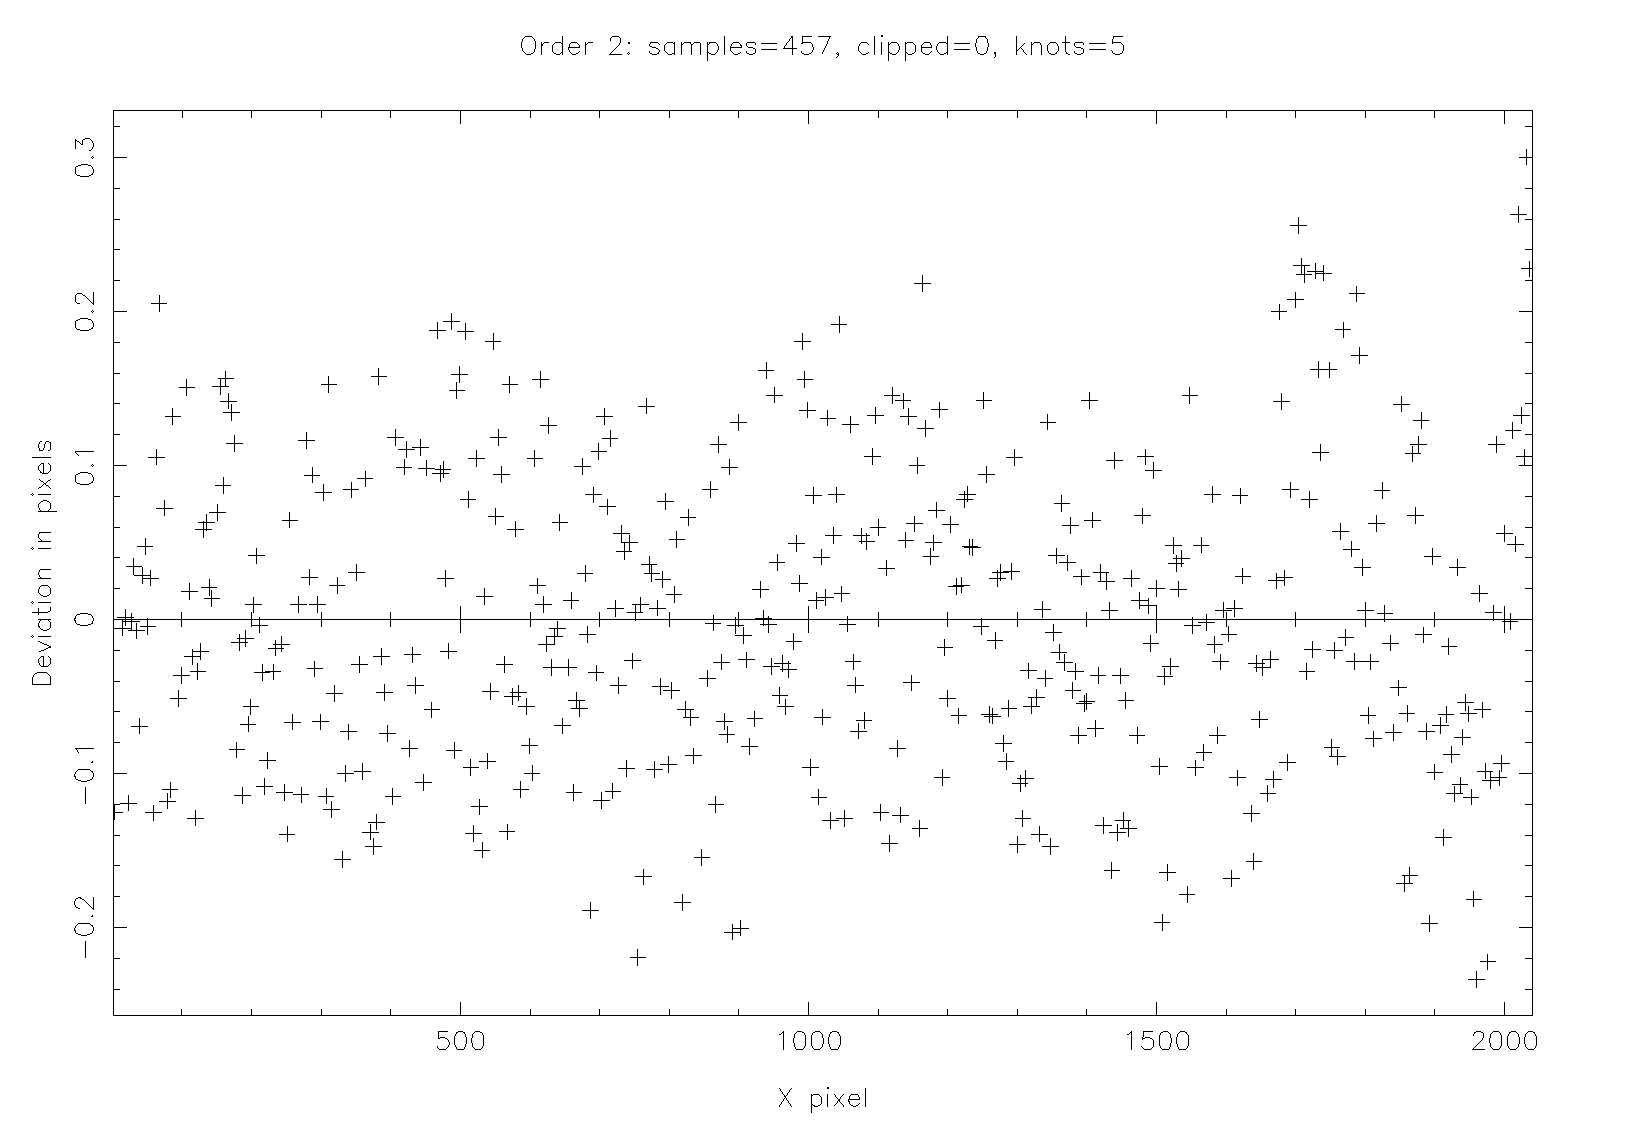
\includegraphics[width=\textwidth]{sun152_02}

\parbox{140mm}{
\caption{A typical plot of the order trace deviations as show during
the trace clipping stage (Option~3).  The points represent the
deviation of the order from the fitted polynomial/spline at a set of
sample column positions.}
\label{fi_tclip}
}
\end{center}
\end{figure}

This routine performs automatic or manual  clipping of points from the
set of samples representing the path of an order across the frame.
A variety of methods of manually clipping points is available, and the degree
of the polynomial used may also be altered. The relationship of the fit
to the trace samples, and the deviations, may be examined graphically.

\begin{figure}
\begin{center}
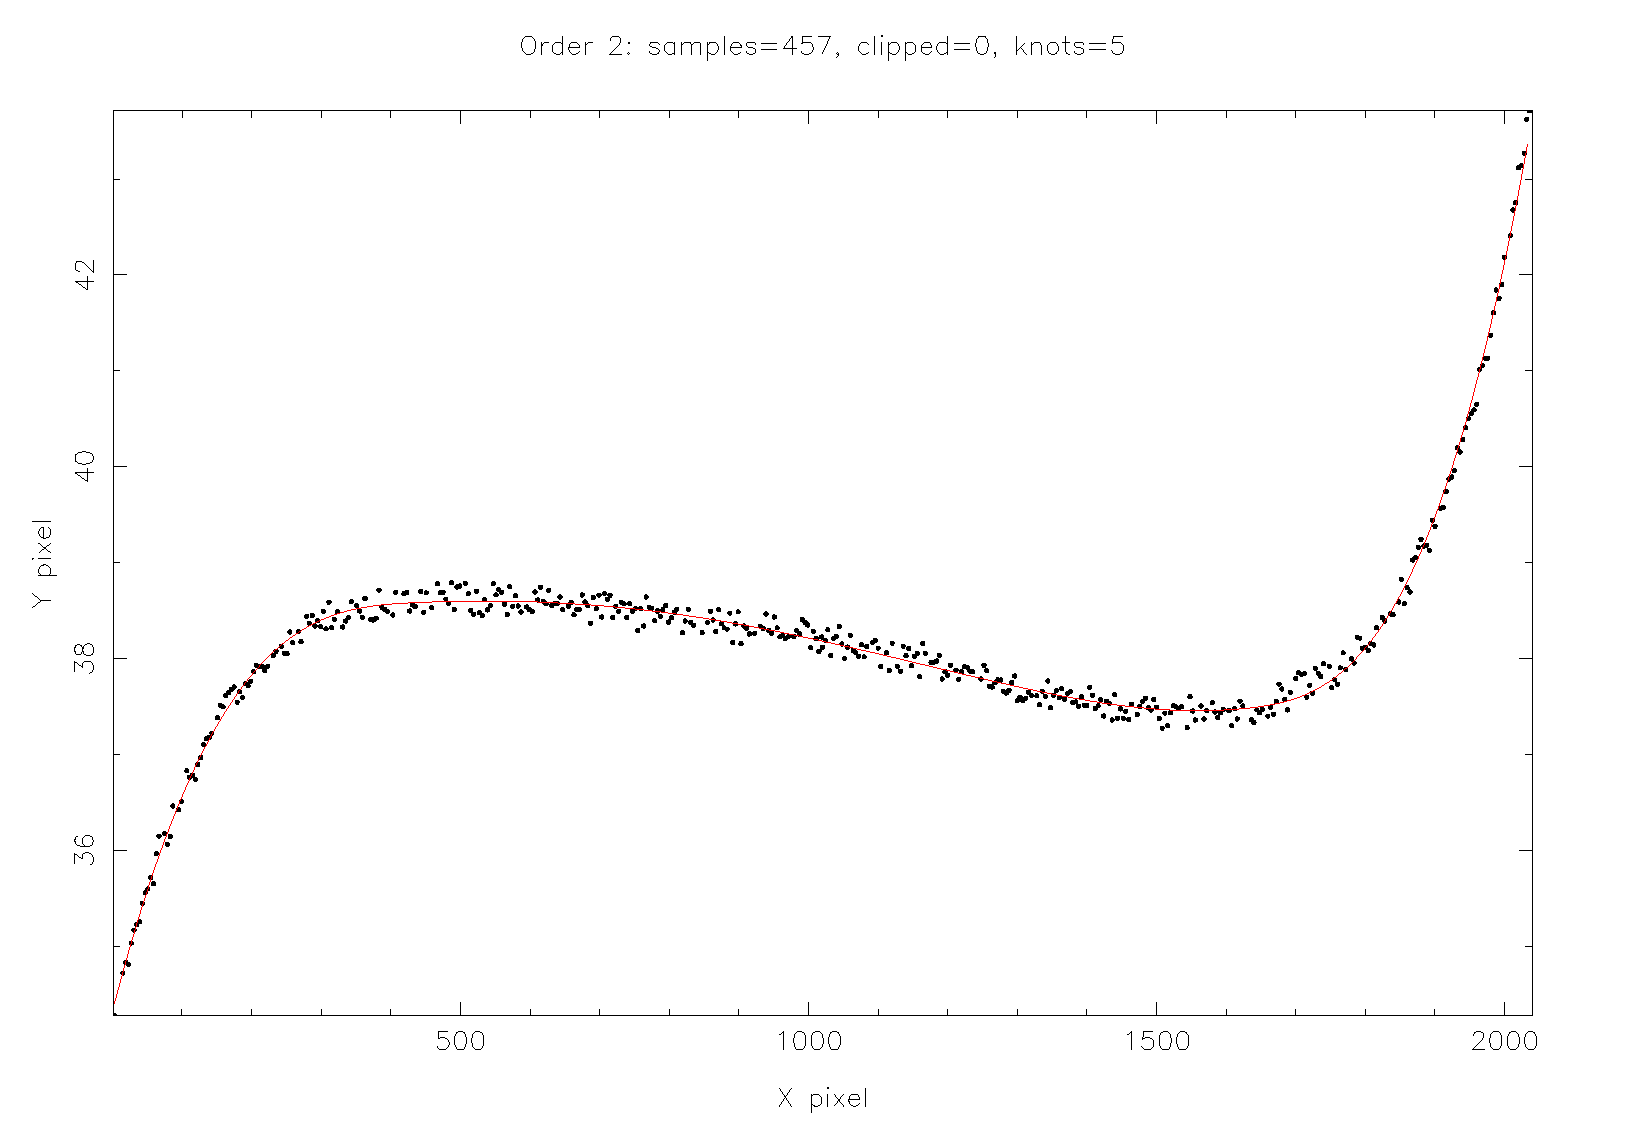
\includegraphics[width=\textwidth]{sun152_03}

\parbox{140mm}{
\caption{A Plot of the fitted order trace overlaid on the trace data.
This plot was made using the option ``V'' in ECHMENU Option 3.}
\label{fi_tracefit}
}
\end{center}
\end{figure}

Orders may be repeatedly re-fitted once they have been initially traced.
In general an automatic fit, clipping to a maximum deviation of third of
a pixel will yield good trace polynomials. The routine may also be used
to remove sets of points which are distorting a fit, for example a run
of bad centre estimates caused by a dodgy column/row.

This routine should be used manually on single orders when they are
clearly not correctly fitted. This will usually be seen by viewing the
paths of the fitted order traces using
\htmlref{{\tt ech\_trplt}}{ech_trplt}\@. In many cases
it will be possible to get a good trace fit by clipping a set of obviously
bad samples, and re-fitting (perhaps with a lower degree of polynomial).

The other main option for coping with such problems is to rely on the trace
consistency checking routine.  This will produce a set of consistent
trace fits in most cases.
\myindex{Order!disabling}
If a particular order is beyond recovery and you do not wish to extract it
at all, then it may be disabled by clipping away all of its trace samples
with this routine.

\sunspec{Figure~\ref{fi_tclip}}{The figure above}
shows an example of the deviations plot after
automatic clipping has been performed on an order.

If you set {\tt TRC\_INTERACT=YES} then a multi-option menu will be displayed.
The options are:

\mlabel{clip_menu}
\begin{itemize}

\item {\sunspec{\Large\tt}{\bf} .}

     Clips the sample nearest to the cursor when the key is pressed.

\item {\sunspec{\Large\tt}{\bf} N}(egative threshold)

     Clips all samples with deviations which are
     {\bf more negative} than the current Y-position of the cursor.

\item {\sunspec{\Large\tt}{\bf} P}(ositive threshold)

     Clips all samples with deviations which are
     {\bf more positive} than the current Y-position of the cursor.


\item {\sunspec{\Large\tt}{\bf} C}(lip)

     Clips all points with absolute deviations greater than the current
     Y-position of the cursor.

\item {\sunspec{\Large\tt}{\bf} R}(ange clip)

     Allows the clipping of a set of samples denoted by a range
     of values along the X-axis of the trace. This will generally be used
     when the order is only partially present, or perhaps to remove
     the contributions of a swath of bad columns. The starting point for
     the range to be clipped is the current cursor X-position, and the
     end point is selected by moving the cursor and hitting any key.

\item {\sunspec{\Large\tt}{\bf} B}(ox clip)

     Like option \texttt{R} but allows you to specify the corners of
     a box in which all samples will be clipped.  Any two corners
     which define the area to be clipped can be used.
     The first corner of the box to be clipped is the current
     cursor X-position; the second (opposite) corner
     is selected by moving the cursor and hitting any key.

\item {\sunspec{\Large\tt}{\bf} A}(utoclip)

     Selects automatic clipping in which points will be
     iteratively clipped and the trace re-fitted. The number of points
     to be clipped is set by {\tt TUNE\_MXCLP}.  If this is zero,
     points are clipped until the absolute deviation of the worst
     sample has fallen below the threshold set by {\tt TUNE\_CLPMAXDEV}.


\item {\sunspec{\Large\tt}{\bf} G}(o)

     Used to switch from interactive clipping to entirely
     automatic mode. Thus after manually clipping a couple of orders
     it may be observed that the orders are well traced and that few
     points need be clipped, this can be left safely to auto-clipping.
     The Go option selects auto-clipping for the current, and any
     subsequent orders.

\item {\sunspec{\Large\tt}{\bf} D}(isable)

     Used when it is clear that the traced samples do not
     follow an order at all and you wish to prevent any subsequent
     processing of the order.  Orders may be automatically disabled
     if a small enough fraction of samples remain after auto-clipping
     has been done.

\item {\sunspec{\Large\tt}{\bf} O}(ff)

     Toggles plotting of the fits; normally a replot occurs for every
     key hit.

\item {\sunspec{\Large\tt}{\bf} F}(unction)

     Rotates the type of fit used.  Currently available types
     are polynomial and spline.

\item {\sunspec{\Large\tt}{\bf} V}(iew)

     The graph used for clipping shows the deviations of each
     sampled trace point. The View option shows the actual coordinates
     of the trace samples, providing an easy reference as to the agreement
     with the order path as expected from visual examination of the raw data.
     {\bf Note} that View mode is mutually exclusive of all other operations
     and must be exited (type any key) before clipping can be resumed.

\item {\sunspec{\Large\tt}{\bf} Q}(uit)

     Leaves the trace fitting for this order without saving
     the trace polynomial in the reduction database. It is therefore
     lost.

\item {\sunspec{\Large\tt}{\bf} E}(xit)

     Leave trace fitting for the current order and save the
     latest trace polynomial in the reduction database.

\item {\sunspec{\Large\tt}{\bf} !}

     Leaves the trace fitting for this order and all subsequent orders.

\item {\sunspec{\Large\tt}{\bf} +}

     Increments the degree of polynomial used to fit
     the trace samples. It may be increased up to the maximum specified
     by {\tt TUNE\_MAXPOLY}.

\item {\sunspec{\Large\tt -}{\bf $-$}}

     Decrements the degree of polynomial used to fit trace samples.

\end{itemize}

\echpars{
\epar{TRCFIT}{Function for trace fitting.}{TRCFIT}
\epar{TRC\_INTERACT}{YES for interactive order-fitting.}{TRC_INTERACT}
\epar{TRC\_NPOLY}{Number of coeffs of trace-fit function.}{TRC_NPOLY}
\epar{TUNE\_CLPBY}{Number of points autoclip before re-fit.}{TUNE_CLPBY}
\epar{TUNE\_CLPMXDEV}{Maximum deviation from polynomial.}{TUNE_CLPMXDEV}
\epar{TUNE\_DIAGNOSE}{YES to log activity to debugging file.}{TUNE_DIAGNOSE}
\lepar{TUNE\_MAXPOLY}{Maximum coefficients for fits.}{TUNE_MAXPOLY}
}

\echredobj{
\eobj{NX\_PIXELS}{\_INTEGER}{READ}
\eobj{TRACE}{\_REAL}{READ}
\eobj{TRC\_CLIPPED}{\_INTEGER}{READ/WRITE}
\eobj{TRC\_IN\_DEV}{\_REAL}{READ/WRITE}
\eobj{TRC\_OUT\_DEV}{\_REAL}{READ/WRITE}
\leobj{TRC\_POLY}{\_DOUBLE}{READ/WRITE}
}


\echtask{option4}{ech_spatial}{4:{\tt ech\_spatial}}{Determine Dekker/Object
 Limits}

\myindex{Dekker limits}
\myindex{Object limits}

The determination of the position of the object data within the slit
proceeds by first locating the slit jaws. To do this either an ARC frame
or (ideally) a flat-field frame may be used. The profile is calculated
along the slit and the edges are then located by determining the points
where the profile intensity drops below a tunable threshold. For
problem cases the dekker positions may also be indicated manually on a
graph of the ARC/Flat field profile.
\myindex{Flat field!defines dekker}
Once the dekker limits have been determined, the object profile is
measured. The object is sampled by averaging the profile over all orders
(using the central columns of the frame only). The median intensity of
the profile inside the dekker limits is then calculated and used to set
an expected sky threshold. The profile is then examined by stepping
outwards from its peak until the profile intensity falls to the expected
sky threshold.
\myindex{Masks!sky/object}
Masks are then created in which
each pixel along the slit is flagged as sky or object. You may also
interactively edit these masks and flag particular sections of the
profile as sky or object. Only pixels flagged as `object' will
contribute to an extraction.
\myindex{Spatially resolved spectra}
Therefore the profile editing provides a (tedious) simple mechanism for
producing spatially resolved spectra (each spatial increment in turn is
flagged as the only object pixel in the profile, and extracted).

The default behaviour is to average all the orders together thus
generating a composite profile. In certain circumstances it may be
necessary to derive a separate profile for each order (for instance for
multi-fibre spectra).  To select this option the parameter
\htmlref{{\tt TUNE\_USE\_NXF=1}}{par_TUNE_USE_NXF} must be set.
\indexcmdname{TUNE_USE_NXF}

This option must be used before any extraction of the orders can take
place. It consists of two steps:

\begin{itemize}

\item \mlabel{ech_dekker} {4.1} (\texttt{ech\_dekker})

      Analyse the Arc/Flat-field frame to determine the positions
      of the edges of the dekker.

\item \mlabel{ech_object} {4.2} (\texttt{ech\_object})

      Analyse the Object frame to determine the position of the
      object within the slit, and its extent above and below the
      traced order.

\end{itemize}

In each case a plot is produced on the graphics device (specified using
the \texttt{SOFT} parameter), showing the status of pixels in relation to their
position relative to the path of the order across the frame.

\begin{figure}
\begin{center}

\includegraphics[width=\textwidth]{sun152_04}

\parbox{140mm}{
\caption{The plot used for dekker limit setting. In interactive use
the cursor is moved to the desired X-position and then either {\tt l}
(for lower) or {\tt u} (for upper) key is pressed to set a limit. If
the scale of the graph is too small then it can be extended by
pressing {\tt l} beyond the left-hand vertical axis, or {\tt u}
beyond the right-hand vertical axis.}
\label{fi_dekker}
}
\end{center}
\end{figure}

\sunspec{Figure~\ref{fi_dekker}}{The Figure above}
shows an example of the dekker plot. The regions
indicated by a solid line are inside the dekker. Pixels in positions
corresponding to the dot/dash line are outside the dekker and will not
be used during processing.

\begin{figure}
\begin{center}

\includegraphics[width=\textwidth]{sun152_05}

\parbox{140mm}{
\caption{The type of plot used for object limit setting. The cursor is
placed at the X-position of the region of interest and then one of
the {\tt o} (object), {\tt s} (sky), {\tt i} (ignore), {\tt b}
(both), keys pressed. Dekker limits may also be changed using the
{\tt u} and {\tt l} keys.}
\label{fi_objlim}
}
\end{center}
\end{figure}

\sunspec{Figure~\ref{fi_objlim}}{The Figure above}
shows an example of the object limits plot. The
regions indicated by a solid line are `object' pixels and will
contribute to the extraction. Regions shown by the dashed line are `sky'
pixels which will be used to calculate the sky model. Pixels in the
dot/dash region are outside the dekker limits and will not be used
during processing.

The pixels' status as set by this option, determine what part they play
when the extraction takes place. That is, it determines if a pixel is
part of the sky, object, outside the slit, or to be ignored completely
by the extraction routine. \indexcmdname{PFL_INTERACT} If the parameter
\htmlref{{\tt PFL\_INTERACT=YES}}{par_PFL_INTERACT} is set then you
are also provided with the opportunity to edit these quantities on a profile
plot.

In addition the limits may be specified by using parameters, which will
over-ride the values calculated by the modules. \myindex{Manual dekker
limits} \myindex{Manual object limits}

\begin{itemize}

\item {\texttt{TUNE\_DEKBLW} to set the lower dekker.}

\item {\texttt{TUNE\_DEKABV} to set the upper dekker.}

\item {\texttt{TUNE\_OBJBLW} to set the lower object limit.}

\item {\texttt{TUNE\_OBJABV} to set the upper object limit.}

\end{itemize}

\myindex{Cosmic rays!when to locate}
After running Option~4, the post-trace cosmic-ray locator may be run if
required (Option~17).  It cannot be used before as it uses the object
limits derived in Option~4.

\echpars{
\epar{INPTIM}{Frame to extract data from.}{INPTIM}
\epar{PFL\_INTERACT}{YES for interactive profiling.}{PFL_INTERACT}
\epar{PFL\_MODE}{Profiling mode (D, S, O, A).}{PFL_MODE}
\epar{SLITIM}{Frame for dekker measurement.}{SLITIM}
\epar{TUNE\_DIAGNOSE}{YES to log activity to debugging file.}{TUNE_DIAGNOSE}
\epar{TUNE\_DEKABV}{Dekker extent in pixels above trace.}{TUNE_DEKABV}
\epar{TUNE\_DEKBLW}{Dekker edge in pixels below trace.}{TUNE_DEKBLW}
\epar{TUNE\_DEKTHR}{Threshold for dekker location.}{TUNE_DEKTHR}
\epar{TUNE\_MAXPOLY}{Maximum coefficients for fits.}{TUNE_MAXPOLY}
\epar{TUNE\_MXSKYPIX}{Maximum number of sky pixels.}{TUNE_MXSKYPIX}
\epar{TUNE\_OBJABV}{Number of object pixels above trace.}{TUNE_OBJABV}
\epar{TUNE\_OBJBLW}{Number of object pixels below trace.}{TUNE_OBJBLW}
\epar{TUNE\_PFLSSAMP}{Maximum number of subsamples in profile.}{TUNE_PFLSSAMP}
\epar{TUNE\_SKYHILIM}{Upper threshold for sky intensity.}{TUNE_SKYHILIM}
\lepar{TUNE\_USE\_NXF}{Fraction of X-samples to use in profile.}{TUNE_USE_NXF}
}

\echredobj{
\eobj{CONTIN\_PROFILE}{\_REAL}{READ/WRITE}
\eobj{DEK\_ABOVE}{\_INTEGER}{READ/WRITE}
\eobj{DEK\_BELOW}{\_INTEGER}{READ/WRITE}
\eobj{NO\_OF\_ORDERS}{\_INTEGER}{READ}
\eobj{NX\_PIXELS}{\_INTEGER}{READ}
\eobj{NY\_PIXELS}{\_INTEGER}{READ}
\eobj{OBJECT\_PROFILE}{\_REAL}{READ/WRITE}
\eobj{OBJ\_MASK}{\_INTEGER}{READ/WRITE}
\eobj{SKY\_MASK}{\_INTEGER}{READ/WRITE}
\leobj{TRC\_POLY}{\_DOUBLE}{READ}
}


\echtask{option5}{ech_ffield}{5:{\tt ech\_ffield}}{Model Flat-field Balance
  Factors}
\myindex{Flat field}
\myindex{Pixel response variations}

The `balance factors' are the per-pixel values which are multiplied into
the raw data to perform the photometric correction required to correct for
differing pixel-to-pixel responses of some detectors (mostly CCDs).

{\sc echomop} will use a flat-field frame if one is available. The flat-field
frame should  be produced using a continuum lamp exposure with the
instrument in an identical configuration to that used for the object
exposure (to ensure that any wavelength dependent behaviour of pixel
response is taken into account). The exposure should be of sufficient
duration to attain high counts in the brightest parts of the image.

{\sc echomop} fits functions in two directions; along the traces, and along the
image columns. The degree of polynomials fitted is tunable, but the
(low) default degree will normally be perfectly reasonable. Each flat-field
pixel in an order is then used to calculate a `balance' factor. This is a
number close to 1 which represents the factor by which a given pixel
exceeds its expected value (predicted by the polynomial).

Note that this technique requires that the flat-field orders vary slowly
and smoothly both along and across each order.

If required many flat-field frames (with identical instrument
configuration) may be co-added prior to {\sc echomop,} and the high S/N flat field
used by {\sc echomop.} At present no special facilities are provided for
calculating the actual error on such a co-added flat field; the expected
error (derived from root-N statistics) is what is used to calculate the
error on the balance factors {\bf unless} appropriate
variances are provides in the flat-field frame error array.
\myindex{Errors!on flat field}
\indexcmdname{FLTFIT}
Other modes of operation are triggered by setting the parameter
\htmlref{\texttt{FLTFIT}}{par_FLTFIT}\@.
If the parameter is set to \texttt{NONE} then no modelling in
the X-direction will be performed. If the parameter is set to \texttt{MEAN},
then no polynomials are  used, but the balance factors are calculated
using the local mean value based  on a 5-pixel sample. This will normally
be used when the flat field at the dekker limits cannot be modelled because
its intensity changes too rapidly on a scale of 1 pixel due to
under-sampling of the profile.

The full set of modelling options is:

\begin{itemize}

\item {\verb+MEAN+}   a local mean parallel to trace.

\item {\verb+MEDIAN+} a local median parallel to trace.

\item {\verb+POLY+}   a polynomial function parallel to trace.

\item {\verb+SPLINE+} bi-cubic spline parallel to trace.

\item {\verb+SMOOTH+} Gaussian smoothing along pixel rows.

\item {\verb+SLOPE+}  local slope along pixel rows.

\item {\verb+NONE+}   all balance factors set to unity.

\end{itemize}

\myindex{User-calculated balance factors}
\indexcmdname{TUNE_PREBAL}
If you produce your own balance-factor frame, then this may be used by
{\sc echomop}.
The parameter \htmlref{{\tt TUNE\_PREBAL}}{par_TUNE_PREBAL}
should then be set to \verb+YES+\@.
In this case no modelling takes place and the balance factors are
simply copied from the frame supplied.
This should be used if the {\sc echomop} models do not generate an appropriate
flat-field.\myindex{Flat field!none}\indexcmdname{TUNE_NOFLAT}
In cases where no flat-field frame is available then the parameter
\htmlref{{\tt TUNE\_NOFLAT=YES}}{par_TUNE_NOFLAT} can be specified;
or, alternatively you can reply \verb+NONE+ when prompted for the name of
the flat-field frame.  In either case, the balance factors will be set to
unity.

\echpars{
\epar{FFIELD}{Name of flat-field image.}{FFIELD}
\epar{FLTFIT}{Fitter for flat-field.}{FLTFIT}
\epar{TUNE\_DIAGNOSE}{YES to log activity to debugging file.}{TUNE_DIAGNOSE}
\epar{TUNE\_FFINTER}{YES for interaction with flat field.}{TUNE_FFINTER}
\epar{TUNE\_FFLMED}{YES for local median, NO for mean.}{TUNE_FFLMED}
\epar{TUNE\_FFLSMP}{Number of local pixels to median/mean.}{TUNE_FFLSMP}
\epar{TUNE\_FFNXREJ}{Reject cycles for X-fits.}{TUNE_FFNXREJ}
\epar{TUNE\_FFNXPLY}{Number of X-coefficients.}{TUNE_FFNXPLY}
\epar{TUNE\_FFNYREJ}{Reject cycles for Y-fits.}{TUNE_FFNYREJ}
\epar{TUNE\_FFNYPLY}{Number of Y-coefficients.}{TUNE_FFNYPLY}
\epar{TUNE\_FFSUBSMP}{YES for subsampling.}{TUNE_FFSUBSMP}
\epar{TUNE\_FFTHRESH}{Reject threshold in sigma.}{TUNE_FFTHRESH}
\epar{TUNE\_MAXPOLY}{Maximum coefficients for fits.}{TUNE_MAXPOLY}
\epar{TUNE\_MXSKYPIX}{Maximum number of sky-pixels.}{TUNE_MXSKYPIX}
\epar{TUNE\_NOFLAT}{YES if no flat-field frame is available.}{TUNE_NOFLAT}
\lepar{TUNE\_PREBAL}{YES for pre-balanced flat field.}{TUNE_PREBAL}
}

\echredobj{
\eobj{DEK\_ABOVE}{\_INTEGER}{READ}
\eobj{DEK\_BELOW}{\_INTEGER}{READ}
\eobj{FITTED\_FLAT}{\_REAL}{READ/WRITE}
\eobj{FLAT\_ERRORS}{\_REAL}{READ/WRITE}
\eobj{NO\_OF\_ORDERS}{\_INTEGER}{READ}
\eobj{NX\_PIXELS}{\_INTEGER}{READ}
\eobj{NY\_PIXELS}{\_INTEGER}{READ}
\leobj{TRC\_POLY}{\_DOUBLE}{READ}
}

\echtask{option6}{ech_sky}{6:{\tt ech\_sky}}{Model Sky Background}
\myindex{Sky!subtraction}

The sky intensity is modelled at each increment along the order.
The degree of polynomial fitted is adjustable, by default it is set to zero
to obtain the `average' sky behavior.

The use of polynomials or splines of higher degree is advisable when there
is a significant gradient to the sky intensity along the slit, as the
polynomials are used to predict the sky intensity at each object pixel
in the order independently.
Note that the meaning of `increment' differs between regular and 2-D
distortion-corrected extractions.
For a simple extraction an increment is a single-pixel column.
For a 2-D extraction each increment is a scrunched wavelength-scale unit,
thus ensuring the accurate modelling of distorted bright emission lines
in the sky.

It is also possible to model the sky intensity in the wavelength
direction using polynomials.
In this case there are parameters available to define the threshold for
possible sky lines which will be excluded from the fit
(\htmlref{{\tt{TUNE\_SKYLINW}}}{par_TUNE_SKYLINW} and
\htmlref{{\tt TUNE\_SKYLTHR}}{par_TUNE_SKYLTHR}).
\indexcmdname{TUNE_SKYLINW}
\indexcmdname{TUNE_SKYLTHR}
\myindex{Sky!noise simulation}
\indexcmdname{TUNE_SKYSIM}
When a wavelength-dependent model is used it is also possible to request
an extra simulation step which allows the accurate evaluation of the
errors on the fitted model (using a monte-carlo simulation). This
procedure can improve the variances used during an `optimal' extraction,
particularly in cases where the object is only fractionally brighter
than the sky.
The simulation is enabled using the hidden parameter
\htmlref{{\tt TUNE\_SKYSIM=YES}}{par_TUNE_SKYSIM}.

The determination of which pixels are sky is done using the masks
set by the profiling task or ECHMENU option.
These masks can be freely edited to cope with any special requirements as
to which regions of the slit are to be used for the sky.
This facility is of particular use when processing frames where
`periscopes' have been used to add in `sky' regions when observing an
extended source.
In such cases, {\sc echomop} currently provides no special
treatment and the periscope sky-pixel positions will have to be edited
into the sky mask using the task \htmlref{{\tt ech\_spatial}/ECHMENU
Option~4}{ech_spatial}.
\indexcmdname{ECH_SPATIAL}

It is also possible to use a separate sky frame by flagging all pixels
as sky, modelling the sky, and then resetting the requisite
object pixels (using Option~4.2) before extracting using the object
frame.

In cases where there is significant contamination of the background due
to scattered light, it is possible to use a global model of the
background intensity instead. \htmlref{{\tt ech\_mdlbck}
(Option~22)}{ech_mdlbck} performs this
process and should be used {\bf instead} of the sky modelling option
(the two processes are mutually exclusive).

\echpars{
\epar{FFIELD}{Name of flat-field image.}{FFIELD}
\epar{INPTIM}{Frame to extract data from.}{INPTIM}
\epar{PHOTON\_TO\_ADU}{Conversion factor for photons.}{PHOTON_TO_ADU}
\epar{READOUT\_NOISE}{Detector readout noise in counts.}{READOUT_NOISE}
\epar{SKYFIT}{Function for sky fitting.}{SKYFIT}
\epar{TUNE\_DIAGNOSE}{YES to log activity to debugging file.}{TUNE_DIAGNOSE}
\epar{TUNE\_MAXPOLY}{Maximum coefficients for fits.}{TUNE_MAXPOLY}
\epar{TUNE\_MXSKYPIX}{Maximum number of sky-pixels.}{TUNE_MXSKYPIX}
\epar{TUNE\_NOFLAT}{YES if no flat-field frame is available.}{TUNE_NOFLAT}
\epar{TUNE\_SKYINTER}{YES if interactive sky-modelling.}{TUNE_SKYINTER}
\epar{TUNE\_SKYLINW}{Maximum expected sky-line width.}{TUNE_SKYLINW}
\epar{TUNE\_SKYLTHR}{Sigma threshold for sky-lines.}{TUNE_SKYLTHR}
\epar{TUNE\_SKYPOLY}{Degree of polynomial to use for sky.}{TUNE_SKYPOLY}
\epar{TUNE\_SKYREJ}{Number of reject cycles.}{TUNE_SKYREJ}
\epar{TUNE\_SKYRTHR}{Reject threshold in sigma.}{TUNE_SKYRTHR}
\epar{TUNE\_SKYSIM}{YES for sky simulation to be used.}{TUNE_SKYSIM}
\lepar{TUNE\_SKYXPLY}{Degree of X-polynomial to use for sky.}{TUNE_SKYXPLY}
}


\echredobj{
\eobj{DEK\_ABOVE}{\_INTEGER}{READ}
\eobj{DEK\_BELOW}{\_INTEGER}{READ}
\eobj{FITTED\_FLAT}{\_REAL}{READ}
\eobj{FITTED\_SKY}{\_REAL}{READ/WRITE}
\eobj{FLAT\_ERRORS}{\_REAL}{READ}
\eobj{FSKY\_ERRORS}{\_REAL}{READ/WRITE}
\eobj{NO\_OF\_ORDERS}{\_INTEGER}{READ}
\eobj{NX\_PIXELS}{\_INTEGER}{READ}
\eobj{NY\_PIXELS}{\_INTEGER}{READ}
\eobj{SKY\_MASK}{\_INTEGER}{READ}
\eobj{SKY\_SPECTRUM}{\_REAL}{READ/WRITE}
\eobj{SKY\_VARIANCE}{\_REAL}{READ/WRITE}
\leobj{TRC\_POLY}{\_DOUBLE}{READ}
}

\echtask{option7}{ech_profile}{7:{\tt ech\_profile}}{Model Object Profile}
\myindex{Object profile}
\myindex{Spatial profile}

The object profile model is constructed by subsampling the profile and may
be an all order average, or independently calculated for each order
(enabled by setting \verb+TUNE_USE_NXF=1+).
\indexcmdname{TUNE_USE_NXF}
\indexcmdname{TUNE_OBJPOLY}
There are also facilities for modelling profiles which vary slowly with
wavelength by fitting polynomials in the wavelength direction (set
\htmlref{{\tt TUNE\_OBJPOLY>0}}{par_TUNE_OBJPOLY}).

\myindex{Spatial subsampling}
\indexcmdname{TUNE_PFLSSAMP}
The degree of subsampling is controlled using the parameter
\htmlref{{\tt TUNE\_PFLSSAMP}}{par_TUNE_PFLSSAMP} which sets the number of
subsamples across the spatial profile.

\echpars{
\epar{INPTIM}{Frame to extract data from.}{INPTIM}
\epar{TUNE\_DIAGNOSE}{YES to log activity to debugging file.}{TUNE_DIAGNOSE}
\epar{TUNE\_MAXPOLY}{Maximum coefficients for fits.}{TUNE_MAXPOLY}
\epar{TUNE\_MXSKYPIX}{Maximum number of sky-pixels.}{TUNE_MXSKYPIX}
\epar{TUNE\_OBJPOLY}{Degree of polynomial to use for object.}{TUNE_OBJPOLY}
\epar{TUNE\_PFLSSAMP}{Maximum number of subsamples in profile.}{TUNE_PFLSSAMP}
\lepar{TUNE\_USE\_NXF}{Fraction of X-samples to use in profile.}{TUNE_USE_NXF}
}

\echredobj{
\eobj{DEK\_ABOVE}{\_INTEGER}{READ}
\eobj{DEK\_BELOW}{\_INTEGER}{READ}
\eobj{FITTED\_SKY}{\_REAL}{READ}
\eobj{MODEL\_PROFILE}{\_REAL}{READ/WRITE}
\eobj{NO\_OF\_ORDERS}{\_INTEGER}{READ}
\eobj{NX\_PIXELS}{\_INTEGER}{READ}
\eobj{NY\_PIXELS}{\_INTEGER}{READ}
\eobj{OBJ\_MASK}{\_INTEGER}{READ}
\eobj{SKY\_MASK}{\_INTEGER}{READ}
\leobj{TRC\_POLY}{\_DOUBLE}{READ}
}


\echtask{option8}{ech_extrct}{8:{\tt ech\_extrct}}{Extract Object and Arc
  Order Spectra}
\myindex{Extraction}

The extraction of both object and arc orders proceeds in parallel to ensure
that the same weights are used in both cases. There are three possible
weighting schemes implemented currently. All methods maintain variances and
allow individual pixels to be excluded from the extraction process by
referring to the object frame quality array.\myindex{Weighting!during extraction}
Simple extraction weights all object pixels equally and is much less
computationally demanding than the other methods. The object intensity is
calculated by summing all the object pixels in each column for each order.

Profile weighted extraction weights each pixel by a factor $P(i,j)^{2}$ where
$P(i,j)$ is the calculated normalised profile at spatial offset $j$
(sub-sampled) from the trace centre and $i$ is the column number.

Optimally weighted (or Variance weighted) extraction weights each pixel by
the product of the calculated profile $P(i,j)$ and an estimate of the
uncertainty of the pixel intensity.

This estimate is based on the calculated variance following the scheme
described by Horne in {\sl An Optimal Extraction Algorithm for CCD
spectroscopy}
(P.A.S.P.~1986), modified to cope with profile subsampling associated with
sloping and/or distorted orders.

In addition, the rejection of cosmic-ray-contaminated pixels has been made
available as a separate function in {\sc echomop} as the package is not dedicated
to CCD-only data reduction.
\myindex{Cosmic rays!using Horne algorithm}
\indexcmdname{TUNE_CRCLEAN}
The original cosmic-ray rejection described by Horne has also been retained
and can be enabled using the parameter
\htmlref{{\tt TUNE\_CRCLEAN}}{par_TUNE_CRCLEAN}, although
the dedicated CR module seems to perform better in most cases.
\myindex{Signal-to-noise, optimal extraction}
Optimally weighted extraction has been shown to improve S/N in the
extracted spectra by factors corresponding to up to 20\% increases in
exposure time, and its use is therefore to be encouraged in most cases. The
provision of sky variance modelling helps to ensure that the optimal
extraction can still perform `optimally' even with very low S/N data.
\myindex{Quick-look extraction}
\myindex{Extraction!quick-look}

\begin{quote}

  {\bf NOTE:} {\sl Option~19---Quick-look extraction is provided
  primarily for at-the-telescope use to permit the observer to quickly
  check that decent data are being obtained. Quick-look does not use the
  sky model or flat-field model and should not be used to produce
  spectra for further analysis.}

\end{quote}

\echpars{
\epar{ARC}{Name(s) of reference (arc) lamp image(s).}{ARC}
\epar{EXTRACT\_MODE}{Extraction mode.}{EXTRACT_MODE}
\epar{FFIELD}{Name of flat-field image.}{FFIELD}
\epar{INPTIM}{Frame to extract data from.}{INPTIM}
\epar{PHOTON\_TO\_ADU}{Conversion factor for photons.}{PHOTON_TO_ADU}
\epar{READOUT\_NOISE}{Detector readout noise in counts.}{READOUT_NOISE}
\epar{TUNE\_CRCLEAN}{YES if Cosmic-Ray clean needed.}{TUNE_CRCLEAN}
\epar{TUNE\_DIAGNOSE}{YES to log activity to debugging file.}{TUNE_DIAGNOSE}
\epar{TUNE\_MAXPOLY}{Maximum coefficients for fits.}{TUNE_MAXPOLY}
\epar{TUNE\_MXSKYPIX}{Maximum number of sky-pixels.}{TUNE_MXSKYPIX}
\epar{TUNE\_NOARC}{YES if no arc frame is available.}{TUNE_NOARC}
\epar{TUNE\_OBJPOLY}{Degree of polynomial to use for object.}{TUNE_OBJPOLY}
\epar{TUNE\_PFLSSAMP}{Maximum number of subsamples in profile.}{TUNE_PFLSSAMP}
\epar{TUNE\_SKVRCORR}{YES to apply sky variance correction.}{TUNE_SKVRCORR}
\epar{TUNE\_SKYPOLY}{Degree of polynomial to use for sky.}{TUNE_SKYPOLY}
\epar{TUNE\_SKYREJ}{Number of reject cycles.}{TUNE_SKYREJ}
\lepar{TUNE\_SKYRTHR}{Reject threshold in sigma.}{TUNE_SKYRTHR}
}

\echredobj{
\eobj{BLAZE\_SPECT}{\_REAL}{READ/WRITE}
\eobj{DEK\_ABOVE}{\_INTEGER}{READ}
\eobj{DEK\_BELOW}{\_INTEGER}{READ}
\eobj{EXTRACTED\_ARC}{\_REAL}{READ/WRITE}
\eobj{EXTRACTED\_OBJ}{\_REAL}{READ/WRITE}
\eobj{EXTR\_ARC\_VAR}{\_REAL}{READ/WRITE}
\eobj{EXTR\_OBJ\_VAR}{\_REAL}{READ/WRITE}
\eobj{FITTED\_FLAT}{\_REAL}{READ/WRITE}
\eobj{FITTED\_PFL}{\_DOUBLE}{READ}
\eobj{FITTED\_SKY}{\_REAL}{READ/WRITE}
\eobj{FLAT\_ERRORS}{\_REAL}{READ/WRITE}
\eobj{FSKY\_ERRORS}{\_REAL}{READ/WRITE}
\eobj{MODEL\_PROFILE}{\_REAL}{READ/WRITE}
\eobj{NO\_OF\_ORDERS}{\_INTEGER}{READ}
\eobj{NX\_PIXELS}{\_INTEGER}{READ}
\eobj{NY\_PIXELS}{\_INTEGER}{READ}
\eobj{OBJ\_MASK}{\_INTEGER}{READ}
\eobj{SKY\_MASK}{\_INTEGER}{READ}
\leobj{TRC\_POLY}{\_DOUBLE}{READ}
}


\echtask{option9}{ech_linloc}{9:{\tt ech\_linloc}}{Locate Arc Line Candidates}

\myindex{Arc line!location}

This option is used to locate arc line features for later identification.
It consists of two steps:

\begin{itemize}

\item \mlabel{ech_fwhm} {9.1} (\verb+ech_fwhm+)

      Determine the average arc line FWHM. \myindex{Arc line!FWHM}

\item \mlabel{ech_lines} {9.2} (\verb+ech_lines+)

      Locate all possible arc lines.

\end{itemize}

\begin{figure}
\begin{center}

\includegraphics[width=\textwidth]{sun152_07}

\parbox{140mm}{
\caption{The ``average'' line-profile for an arc.  This was produced using
ECHMENU Option 9.}
\label{fi_linewidth}
}
\end{center}
\end{figure}

The FWHM is evaluated by co-adding all possible arc line features in the
arc frame, and then averaging the resulting profile, and calculating its
FWHM. The value is used to scale the Gaussian-s which are fitted to each
arc line in order to obtain an estimate of its center position (in X).

Possible arc lines are denoted by any region of an order in which 5
consecutive pixels (P1\sunspec{--}{-}5) obey the following relation:

\begin{displaymath}
P_{1} < P_{2} < P_{3} > P_{4} > P_{5}
\end{displaymath}

%P1 less than P2 less than P3 greater than P4 greater than P5

and are amenable to a Gaussian fit with the FWHM calculated.

This ensures that even very faint features are put forward for possible
identification (useful when there are no bright lines in an entire
order).

\echpars{
\epar{ARC}{Name(s) of reference (arc) lamp image(s).}{ARC}
\epar{TUNE\_DIAGNOSE}{YES to log activity to debugging file.}{TUNE_DIAGNOSE}
\epar{TUNE\_MAXPOLY}{Maximum coefficients for fits.}{TUNE_MAXPOLY}
\epar{TUNE\_MAXRFLN}{Maximum number of reference lines.}{TUNE_MAXRFLN}
\epar{TUNE\_NOARC}{YES if no arc frame is available.}{TUNE_NOARC}
\lepar{TUNE\_RFLNTHR}{Reference line lower threshold.}{TUNE_RFLNTHR}
}


\echredobj{
\eobj{EXTRACTED\_ARC}{\_REAL}{READ/WRITE}
\eobj{NO\_OF\_ORDERS}{\_INTEGER}{READ}
\eobj{NREF\_FRAME}{\_INTEGER}{READ}
\eobj{NX\_PIXELS}{\_INTEGER}{READ}
\eobj{NY\_PIXELS}{\_INTEGER}{READ}
\eobj{OBS\_INTEN}{\_REAL}{READ/WRITE}
\eobj{OBS\_LINES}{\_REAL}{READ/WRITE}
\eobj{REF\_LINE\_FWHM}{\_REAL}{READ/WRITE}
\leobj{TRC\_POLY}{\_DOUBLE}{READ}
}


\echtask{option10}{ech_idwave}{10:{\tt ech\_idwave}}{Wavelength Calibrate}
\myindex{Wavelength calibration}
\myindex{Arc line!calibration}

The wavelength calibration is done using a reference feature list, usually
provided by an ARC-lamp exposure. The routine allows any candidate features
to be identified and used as `knowns' for the calibration (as
position/intensity pairs). These features may then be manually identified
using a reference lamp atlas. Facilities are provided for adding/deleting
lines and altering the degree of polynomial fit performed.

An automatic line-identifier is included which operates by searching the
supplied line list for multi-line `features'.
You may optimise the search by constraining the space to be searched in
terms of permissible wavelength and/or dispersions (in Angstroms/pixel).

In addition the program will automatically constrain the search range
further if it can determine the central order number and wavelength (by
looking in the data frame header)

As soon as three orders have been successfully calibrated, the search range
for the remaining orders is re-evaluated to take this into account.
In general, the automatic method will be most useful when you are unsure of
the exact wavelength range covered.  When the level of doubt is such that
the wavelength scale may decrease from left-to-right across the frame, then
the software may be instructed to automatically check for this `reversed'
condition.
Set parameter \htmlref{{\tt TUNE\_REVCHK}}{par_TUNE_REVCHK} to \verb+YES+
to check for a reversed arc; the parameter defaults to \verb+NO+ to avoid
wasting CPU time.
If the wavelength scale is reversed then you should use
\xref{{\sc figaro}}{sun86}{}
\xref{IREVX}{sun86}{IREVX} to flip all the relevant images, and then re-start
the reduction.

\myindex{Wavelength scales!reversed}
\indexcmdname{TUNE_REVCHK}
Finally the software is flexible as to the vertical orientation of the
orders, {\it{i.e.}}, higher wavelength orders may be at the top or bottom
of the frame (for \'{e}chelle data).
\myindex{Orientation of frames}
Calibration may be performed using either 1 or 2 (before and after) ARC
frames at present.  See \sunspec{\S\ref{arc_frames}}
{\htmlref{Arc Frames}{arc_frames}} for details.

Options are presented in a menu form and selected by typing a one or two
character string, followed by carriage return.  The following options are
supported:

\begin{itemize}

\item {\sunspec{\Large\tt}{\bf} AI} (automatic identification)

      Initiates a search and
      match of the feature database. Any preset limitations on the
      wavelength and dispersion range will be taken into account. When a
      solution is found, a fit report includes a probable status.
      You may then refine the solution manually, or search for
      further solutions by hitting the A key.


\item {\sunspec{\Large\tt}{\bf} E}(xit)

      Leaves the line identification menu and
      updates the reduction database copy of the wavelength polynomial to
      reflect the latest calculated fit.

\item {\sunspec{\Large\tt}{\bf} H}(elp)

      Provides interactive browsing of the relevant
      sections of the help library for line identification.

\item {\sunspec{\Large\tt}{\bf} IM} (import \xref{ECHARC}{sun86}{ECHARC} data)
%\myindex{ECHARC!data exchange}
\myindex{ECHARC data exchange@\protect\cmdname{ECHARC} data exchange}
      Provides an interface
      to the ECHARC arc-line identification program. In general the XP
      option should first be used to export data for ECHARC processing.
      ECHARC would then be run, and finally the data IMported back into
      {\sc echomop}.

\item {\sunspec{\Large\tt}{\bf} O}(rder selection)

      Used to change the currently
      selected order when operating manually. The order number which is to
      be selected will be prompted for.

\item {\sunspec{\Large\tt}{\bf} P}(olynomial degree)

      Used to alter the degree of
      polynomial to be used for the wavelength fitting. This may vary up to
      the maximum set by \htmlref{{\tt TUNE\_MAXPOLY}}{par_TUNE_MAXPOLY}\@.

\item {\sunspec{\Large\tt}{\bf} XP} (export data for ECHARC)

      Used to provide an
      interface to the ECHARC arc line identification program. In general
      the XP option should first be used to export data for ECHARC
      processing. ECHARC would then be run, and finally the data IMported
      back into {\sc echomop}.

\item {\sunspec{\Large\tt}{\bf} I}(nteractive identification)

      Enters the interactive
      line specification, examination section. This section has a menu
      which provides features for addition/deletion/re-fitting/listing {\it
      etc.}, of identified lines.

      This sub-menu includes a set of interactive options to assist in
      identifying arc lines and fitting the wavelength polynomial to
      describe the variation along an order. The options provided are as
      follows and are all selected using a single character. Note that the
      carriage-return key is not necessary for option selection, care is
      therefore needed to ensure that the cursor is correctly positioned
      {\bf before} a cursor dependent option is selected.

      \begin{itemize}

      \item {\sunspec{\Large\tt}{\bf} A}(uto)

            Initiates an automatic search and match of
            the reference feature database. Any preset limits on the
            wavelength and dispersion search range are taken into account.
            Each possible solution is reported upon with an indication of
            its probable accuracy.  You may then choose to reject it,
            or examine it in detail for verification or modification.

      \item {\sunspec{\Large\tt}{\bf} B}(Clip)
            \myindex{Arc fitting!blends}
            Automatically clips any potential blends
            from the set of identified lines, and re-fits the wavelength
            polynomial. Possible blends are flagged using the identifier B
            on the graph, and by a trailing B on the line details output
            during fits.

      \item {\sunspec{\Large\tt}{\bf} C}(lear all identifications)
            \myindex{Arc fitting!clear}

            Removes all
            identified line information for the order. The polynomial fit
            remains though, and any good lines could be recovered by using
            the R(e-interpolate) option.

      \item {\sunspec{\Large\tt}{\bf} D}(elete a line)
            \myindex{Arc fitting!delete line}

            Removes an identified line from
            the set of identified lines. This will usually be used to
            remove a suspect line which has been incorrectly automatically
            identified. The identified line nearest to the cursors
            X-position when the D is pressed,  will be the one which is
            deleted.

      \item {\sunspec{\Large\tt}{\bf} E}(xit)

            Leaves the interactive
            identification/fitting routine and returns to the main line id
            menu. The current set of fitted lines,  and the polynomial are
            saved in the reduction database.

      \item {\sunspec{\Large\tt}{\bf} F}(it polynomial)

            Performs a polynomial fit to
            the positions/wavelengths of all currently identified lines.
            Reports on the deviation of each line from the fit,  and the
            improvement possible by deleting each line and re-fitting. No
            check is made against the database to see if further lines may
            now be identified, use the R option if this is required.

      \item {\sunspec{\Large\tt}{\bf} I}(nformation)

            Reports information known about
            the nearest located line (relative to X-position of cursor when
            I is pressed). Details include position, wavelength {\it etc.}

      \item {\sunspec{\Large\tt}{\bf} K}(eep)

            Flags the nearest identified-line to
            be retained during re-interpolation even when it
            would otherwise be rejected. Any manually identified lines will
            be automatically flagged in this way. Kept lines are indicated
            by a K on the graph.

      \item {\sunspec{\Large\tt}{\bf} L}(ist known lines)
            \myindex{Arc fitting!list known lines}

            Examines the feature database
            to find the nearest features to the current X-position of the
            cursor,  assuming the current polynomial fits' predictions
            about the corresponding wavelengths.

      \item {\sunspec{\Large\tt}{\bf} M}(ove to coordinate)

            When viewing a zoomed graph
            of lines, allows the central point of the plot to be moved to
            any point along the X-axis. A prompt is made for the exact
            co-ordinate required. Once a wavelength scale has been fitted,
            Move operates on wavelengths, otherwise it operates on
            X-coordinates.

      \item {\sunspec{\Large\tt}{\bf} N}(ew line)
            \myindex{Arc fitting!new line}

            Used to specify a completely new
            feature. Should be used when you wish to identify a line which
            has not been located at all by the arc line location algorithm.
            All located lines brighter than the threshold (see Threshold
            option) are indicated by a \(\mid\) appearing above their peak.
            Identified lines additionally have the wavelength shown.

      \item {\sunspec{\Large\tt}{\bf} O}(utwards zoom)

            Reverses any currently selected
            zoom factor on the displayed graph of lines.

      \item {\sunspec{\Large\tt}{\bf} P}(lot)

            Refreshes the plotted graph.

      \item {\sunspec{\Large\tt}{\bf} Q}(uit)

            Leaves the manual identification/fitting
            routine {\bf without} updating the polynomial in the reduction
            database.

            \begin{quote}

               {\bf NOTE:} {\sl any newly identified lines will be saved.
               Only the polynomial (which represents the outcome of an
               identification) is left unchanged.}

            \end{quote}

      \item {\sunspec{\Large\tt}{\bf} R}(e-interpolate)

            A polynomial fit is made to the
            currently identified lines. This polynomial is then used to
            search the database for any new line candidates. All new
            candidates are then added into the fit and the polynomial
            iteratively re-fitted and clipped until a stable solution is
            obtained.

      \item {\sunspec{\Large\tt}{\bf} S}(et line wavelength)
            \myindex{Arc fitting!set wavelength}

            Used to set the
            wavelength of a line. The line whose wavelength is to be set
            should be the one nearest to the X-position of the cursor and
            may be an identified or unidentified line. Use the N(ew) option
            to create a new line where none had been auto-located.

      \item {\sunspec{\Large\tt}{\bf} T}(hreshold)

            Used to set the threshold for
            identifiable lines. Only identifiable lines can be
            automatically identified by the Auto or Re-interpolate options.
            The threshold is plotted on the graph as a horizontal dotted
            line and is initially set according to the value of the
            parameter \htmlref{{\tt TUNE\_IDSTRNG}}{par_TUNE_IDSTRNG}\@.

      \item {\sunspec{\Large\tt}{\bf} XCLIP}

            Used to toggle automatic clipping of
            poorly fitted lines.  It is checked every time a fit is
            performed and when set will allow the fitting module to reject
            lines if doing so will significantly improve the RMS for the
            fit.

      \item {\sunspec{\Large\tt}{\bf} Z}(oom plot)

            Increases the magnification of the
            graph used to plot the line positions. To reverse the effect
            use the O(utwards zoom) option.

      \item {\sunspec{\Large\tt}{\bf} +} (Increment polynomial order)

            Increments the degree
            of polynomial used for the wavelength fitting. May be increased
            up to the maximum specified by the parameter
            \htmlref{{\tt TUNE\_MAXPOLY}}{par_TUNE_MAXPOLY}\@.

      \item {\sunspec{\Large\tt}{\bf} -} (Decrement polynomial order)

            Decrements the degree
            of polynomial used for the wavelength fitting.

      \item {\sunspec{\Large}{\bf} \texttt{>}} (Shift display right)

            When a zoomed graph is
            plotted, will shift the viewpoint along to the right (plus X)
            by an amount sufficient to show the adjacent section of the
            plot.

      \item {\sunspec{\Large}{\bf} \texttt{<}} (Shift display left)

            When a zoomed graph is plotted,
            will shift the viewpoint along to the left (minus X) by an
            amount sufficient to show the adjacent section of the plot.
            (any other key), provides available information on the line
            nearest to the current X-position of the cursor.

      \item {\sunspec{\Large\tt}{\bf} =}

            Switches between fitting functions.
            Currently supported are polynomials and splines.

      \item {\sunspec{\Large\tt}{\bf} \verb+^+}
            \myindex{Arc fitting!hardcopies}

            Sends a copy of the current plotted graph to the hardcopy device.
            The appropriate device must have been supplied at program startup
            ({\it{e.g.}} \verb+echmenu hard=ps_l+).

      \end{itemize}

\end{itemize}

\begin{figure}
\begin{center}
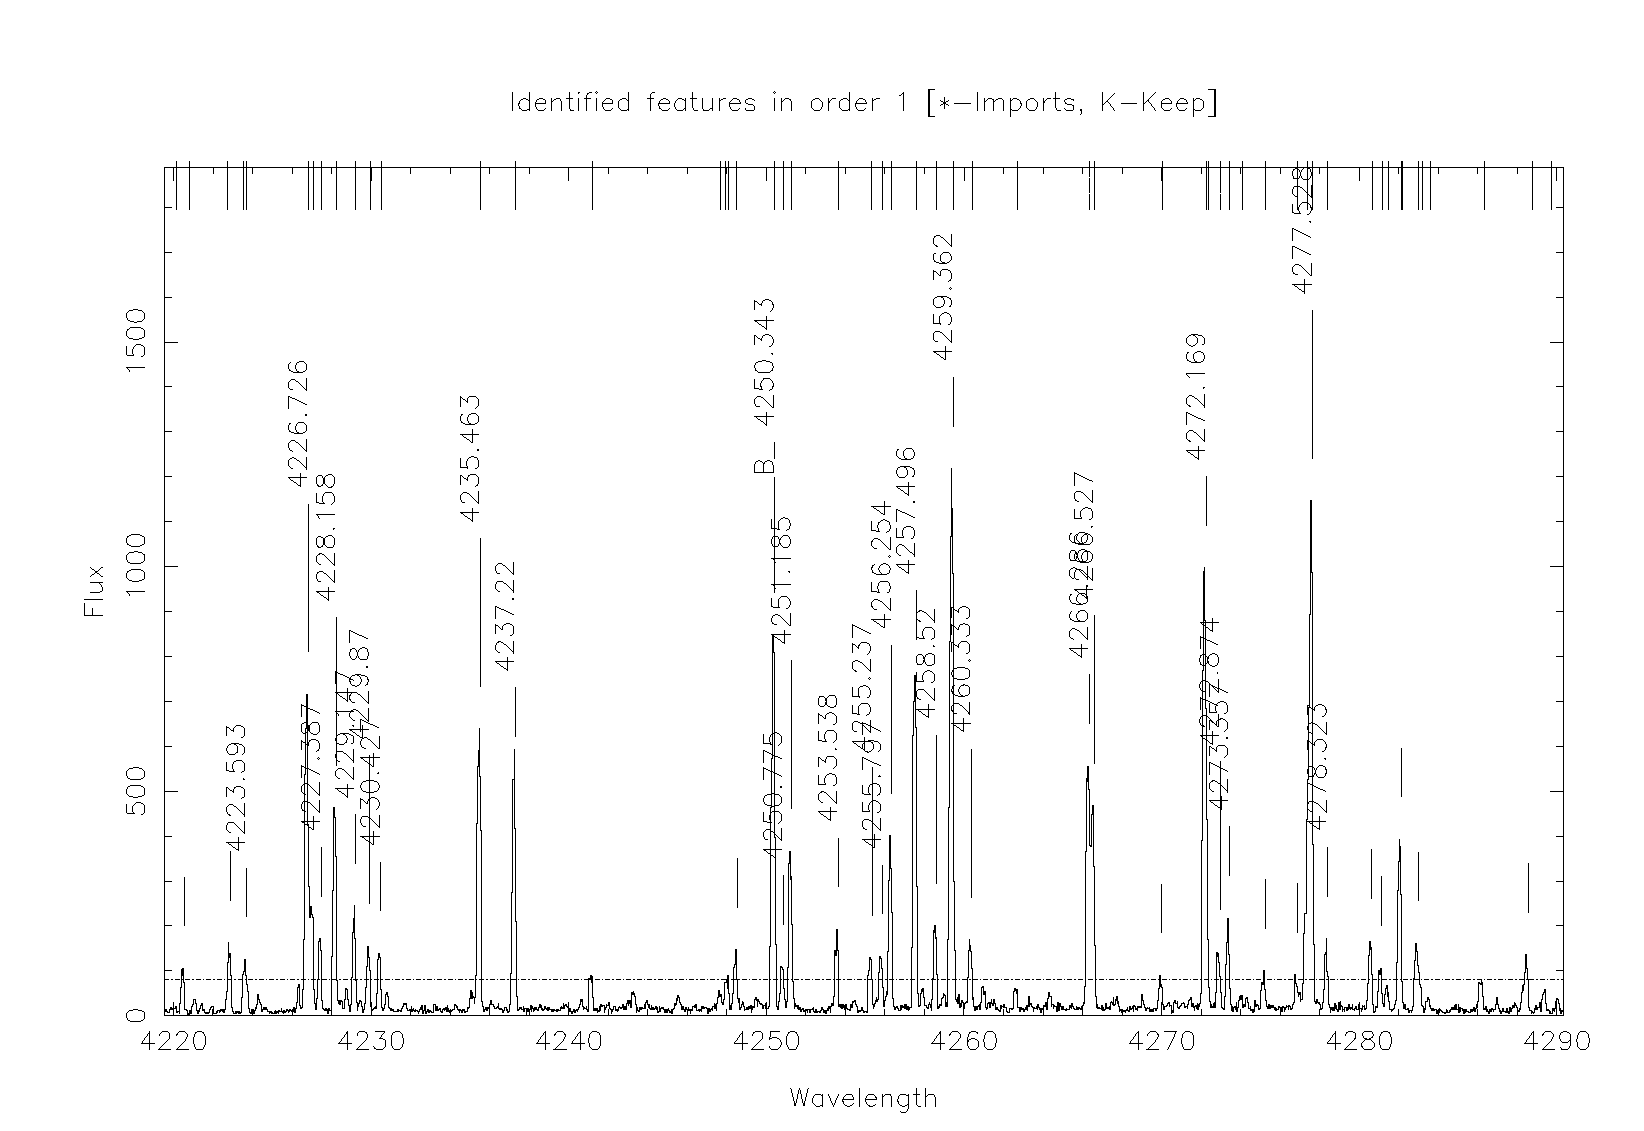
\includegraphics[width=\textwidth]{sun152_06}

\parbox{140mm}{
\caption{A typical plot during interactive line-identification.}
\label{fi_idline}
}
\end{center}
\end{figure}

\sunspec{Figure~\ref{fi_idline}}{The Figure above}
shows an example of the plot displayed during interactive line-identification.
The following points should be noted:

\begin{itemize}
\item Identified lines have their wavelength shown directly above the peak
\item Possible blends are flagged with a B
\item The threshold intensity for identifiable lines is shown as a horizontal
dot/dash line
\item The positions of line-list lines are shown along the top X-axis
\end{itemize}

\echpars{
\epar{AUTO\_ID}{YES for fully automatic identification.}{AUTO_ID}
\epar{CENTRAL\_ONUM}{Hidden parameter.}{CENTRAL_ONUM}
\epar{CENTRAL\_WAVE}{Hidden parameter.}{CENTRAL_WAVE}
\epar{ECH\_FTRDB}{Reference line list database.}{ECH_FTRDB}
\epar{HI\_WAVE}{Longest wavelength to search for arc lines.}{HI_WAVE}
\epar{LOW\_WAVE}{Shortest wavelength to search for arc lines.}{LOW_WAVE}
\epar{MAX\_DISPERSION}{Max dispersion (Units per-pixel) allowed.}{MAX_DISPERSION}
\epar{MIN\_DISPERSION}{Min dispersion (Units per-pixel) allowed.}{MIN_DISPERSION}
\epar{TUNE\_DB\_SCOPE}{Scope of database neighbour scanning.}{TUNE_DB_SCOPE}
\epar{TUNE\_DIAGNOSE}{YES to log activity to debugging file.}{TUNE_DIAGNOSE}
\epar{TUNE\_IDINMN}{Minimum number of features used.}{TUNE_IDINMN}
\epar{TUNE\_IDINMX}{Maximum number of features used.}{TUNE_IDINMX}
\epar{TUNE\_IDMDLT}{Maximum neighbours to check.}{TUNE_IDMDLT}
\epar{TUNE\_IDMXDIF}{Maximum ratio difference.}{TUNE_IDMXDIF}
\epar{TUNE\_IDSDLT}{Starting number of neighbours to check.}{TUNE_IDSDLT}
\epar{TUNE\_IDSTRNG}{Minimum strength of identified lines.}{TUNE_IDSTRNG}
\epar{TUNE\_MAXPOLY}{Maximum coefficients for fits.}{TUNE_MAXPOLY}
\epar{TUNE\_MAXRFLN}{Maximum number of reference lines.}{TUNE_MAXRFLN}
\epar{TUNE\_REVCHK}{Maximum number of reference lines.}{TUNE_REVCHK}
\epar{W\_NPOLY}{Number of coeffs of wavelength fitting function.}{W_NPOLY}
\lepar{WAVFIT}{Function for wavelength fitting.}{WAVFIT}
}


\echredobj{
\eobj{EXTRACTED\_ARC}{\_REAL}{READ}
\eobj{FITTED\_WAVES}{\_DOUBLE}{READ/WRITE}
\eobj{ID\_COUNT}{\_INTEGER}{READ/WRITE}
\eobj{ID\_LINES}{\_REAL}{READ/WRITE}
\eobj{ID\_STATUS}{\_INTEGER}{READ/WRITE}
\eobj{ID\_WAVES}{\_REAL}{READ/WRITE}
\eobj{NO\_OF\_ORDERS}{\_INTEGER}{READ}
\eobj{NREF\_FRAME}{\_INTEGER}{READ}
\eobj{NX\_PIXELS}{\_INTEGER}{READ}
\eobj{OBS\_INTEN}{\_REAL}{READ/WRITE}
\eobj{OBS\_LINES}{\_REAL}{READ/WRITE}
\eobj{ORDER\_IDNUM}{\_INTEGER}{READ/WRITE}
\eobj{REF\_LINE\_FWHM}{\_REAL}{READ/WRITE}
\eobj{WSEAR\_END}{\_REAL}{READ/WRITE}
\eobj{WSEAR\_START}{\_REAL}{READ/WRITE}
\leobj{W\_POLY}{\_DOUBLE}{READ/WRITE}
}


\echtask{option11}{ech_blaze}{11:{\tt ech\_blaze}}{Fit and Apply Ripple
  Correction}
\myindex{Order!blaze}
\myindex{Ripple correction}

This option consists of two steps as follows:

\begin{itemize}

\item \mlabel{ech_fitblz} {11.1} ({\tt{ech\_fitblz}})
      Model blaze function using a polynomial.

\item \mlabel{ech_doblz} {11.2} ({\tt{ech\_doblz}})
      Apply blaze function to extracted spectrum.

\end{itemize}

If flux calibration is not being performed it is sometimes desirable to
remove the `blaze' function from the extracted spectrum to assist in
fitting line profiles {\it etc.} during data analysis.

A task is provided for this purpose which operates by fitting curves
to the flat-field orders.  The curves can be polynomials, splines or
simple fits based on local-median values.  The fits may be automatically or
interactively clipped and the resulting blaze spectrum is normalised such
that its median intensity is unity.

The normalised blaze is then divided into the extracted spectrum. It is
important to remember that this operation is performed upon the `extracted'
spectrum.

\indexcmdname{TUNE_BLZRSET}
After a blaze function has been applied to the extracted order all its
values may be reset to unity to ensure that the order(s) cannot be
re-flattened in error
(\htmlref{{\tt{TUNE\_BLZRSET=YES}}}{par_TUNE_BLZRSET}).  If the
blaze is to be re-applied then the correct procedure is to first
re-extract the order(s) concerned and then re-fit the blaze.

\echpars{
\epar{BLZFIT}{Function for blaze fitting.}{BLZFIT}
\epar{BLZ\_INTERACT}{YES for interactive blaze-fitting.}{BLZ_INTERACT}
\epar{BLZ\_NPOLY}{Number of coeffs of blaze fitting function.}{BLZ_NPOLY}
\epar{FFIELD}{Name of flat-field image.}{FFIELD}
\epar{TUNE\_BLZRSET}{YES if blaze function to be reset after use.}{TUNE_BLZRSET}
\epar{TUNE\_DIAGNOSE}{YES to log activity to debugging file.}{TUNE_DIAGNOSE}
\epar{TUNE\_MAXPOLY}{Maximum coefficients for fits.}{TUNE_MAXPOLY}
\epar{TUNE\_NOFLAT}{YES if no flat-field frame is available.}{TUNE_NOFLAT}
\lepar{TUNE\_YBLAZE}{YES for Y-blaze correction.}{TUNE_YBLAZE}
}


\echredobj{
\eobj{BLAZE\_MEDIANS}{\_REAL}{READ/WRITE}
\eobj{BLAZE\_SPECT}{\_REAL}{READ/WRITE}
\eobj{DEK\_ABOVE}{\_INTEGER}{READ}
\eobj{DEK\_BELOW}{\_INTEGER}{READ}
\eobj{EXTRACTED\_OBJ}{\_REAL}{READ/WRITE}
\eobj{EXTR\_OBJ\_VAR}{\_REAL}{READ/WRITE}
\eobj{FITTED\_WAVES}{\_DOUBLE}{READ}
\eobj{NO\_OF\_ORDERS}{\_INTEGER}{READ}
\eobj{NREF\_FRAME}{\_INTEGER}{READ}
\eobj{NX\_PIXELS}{\_INTEGER}{READ}
\eobj{NY\_PIXELS}{\_INTEGER}{READ}
\eobj{TRC\_OUT\_DEV}{\_REAL}{READ}
\leobj{TRC\_POLY}{\_DOUBLE}{READ}
}


\echtask{option12}{ech_scrunch}{12:{\tt ech\_scrunch}}{Scrunch}
\myindex{Scrunching}

This option is used to scrunch the extracted order spectra (and arc order
spectra) into a (usually) linear wavelength scale.

\begin{itemize}

\item \mlabel{ech_fitfwhm} {12.1} ({\tt{ech\_fitfwhm}})

      Fit reference line FWHM as a function of wavelength

\item \mlabel{ech_fit_wscale} {12.2} ({\tt{ech\_wscale}})

      Calculate the wavelength scale

\item \mlabel{ech_scrobj} {12.3} ({\tt{ech\_scrobj}})

      Scrunch the extracted object order

\item \mlabel{ech_scrarc} {12.4} ({\tt{ech\_scrarc}})

      Scrunch the extracted arc  orders

\end{itemize}

\myindex{FIGARO!SCRUNCH}
The scrunching of spectra into a linear wavelength scale provides exactly
the same facilities available using the \xref{{\sc figaro}}{sun86}{}
\xref{SCRUNCH}{sun86}{SCRUNCH} program, except that it works on an
order-by-order basis.

{\sc echomop} provides both global (bin size constant for all orders) and
per-order scrunching options. The global option would normally be used when
it is necessary to co-add the extracted orders from multiple data frames,
and a standard bin-size is required.

Scrunching results in both a 2-D array of scrunched individual orders, and a
merged 1-D array of the whole wavelength range.
\myindex{Multiple object frames}
\myindex{Merge multiple spectra}
\myindex{Weighting!during co-addition}
A utility (Option~21) is provided to assist in the co-adding of spectra
from many frames together. This option assumes that the first frame in the
reduction has been scrunched with the required wavelength scale. It then
reads a list of additional reduction database names (or EXTOBJ result
file names) from an ASCII file called {\tt NAMES.LIS}. The extracted
spectra from each of these reduction files are then scrunched to the same
scale and co-added into the scrunched spectra in the current reduction
file. The type of weighting during addition is controlled using the
parameter \htmlref{{\tt TUNE\_MRGWGHT}}{par_TUNE_MRGWGHT}\@.

\echpars{
\epar{BIN\_SIZE}{Bin size for global scrunch.}{BIN_SIZE}
\epar{SCRUNCH\_TYPE}{Type of spectrum to scrunch.}{SCRUNCH_TYPE}
\epar{SET\_WSCALE}{YES to scrunch to a global bin size.}{SET_WSCALE}
\epar{START\_WAVE}{Start wavelength for rebinned scale.}{START_WAVE}
\epar{TUNE\_DIAGNOSE}{YES to log activity to debugging file.}{TUNE_DIAGNOSE}
\epar{TUNE\_FLUX}{YES if flux is to be conserved.}{TUNE_FLUX}
\epar{TUNE\_INTR}{YES if linear interpolation required.}{TUNE_INTR}
\epar{TUNE\_LOG}{YES if output scale logarithmic.}{TUNE_LOG}
\epar{TUNE\_MAXPOLY}{Maximum coefficients for fits.}{TUNE_MAXPOLY}
\epar{TUNE\_MAXRFLN}{Maximum number of reference lines.}{TUNE_MAXRFLN}
\epar{TUNE\_MERGE}{YES for merging multiple frame data.}{TUNE_MERGE}
%\epar{TUNE\_MRGWGHT}{Type of weighting to apply.}{TUNE_MRGWGHT}
\epar{TUNE\_QUAD}{YES if quadratic interpolation required.}{TUNE_QUAD}
\epar{TUNE\_SCFRACT}{Fractional ratio for twin scales.}{TUNE_SCFRACT}
\epar{TUNE\_SCRADD}{Number of bins to add together.}{TUNE_SCRADD}
\epar{TUNE\_SCRMODE}{Scrunching mode control.}{TUNE_SCRMODE}
\epar{TUNE\_SKEW}{Skew shift in bins.}{TUNE_SKEW}
\lepar{TUNE\_YBLAZE}{YES for Y-blaze correction.}{TUNE_YBLAZE}
}

\echredobj{
\eobj{BLAZE\_SPECT}{\_REAL}{READ}
\eobj{ERR\_SPECTRUM}{\_REAL}{READ/WRITE}
\eobj{EXTRACTED\_ARC}{\_REAL}{READ}
\eobj{EXTRACTED\_OBJ}{\_REAL}{READ}
\eobj{EXTR\_ARC\_VAR}{\_REAL}{READ}
\eobj{EXTR\_OBJ\_VAR}{\_REAL}{READ}
\eobj{ID\_COUNT}{\_INTEGER}{READ}
\eobj{ID\_LINES}{\_REAL}{READ}
\eobj{ID\_WAVES}{\_REAL}{READ}
\eobj{ID\_WIDTHS}{\_REAL}{READ/WRITE}
\eobj{NO\_OF\_BINS}{\_INTEGER}{READ/WRITE}
\eobj{NO\_OF\_ORDERS}{\_INTEGER}{READ}
\eobj{NREF\_FRAME}{\_INTEGER}{READ}
\eobj{NX\_PIXELS}{\_INTEGER}{READ}
\eobj{NX\_REBIN}{\_INTEGER}{READ/WRITE}
\eobj{REF\_LINE\_FWHM}{\_REAL}{READ}
\eobj{SCRNCHD\_ARC}{\_REAL}{READ/WRITE}
\eobj{SCRNCHD\_ARCV}{\_REAL}{READ/WRITE}
\eobj{SCRNCHD\_OBJ}{\_REAL}{READ/WRITE}
\eobj{SCRNCHD\_OBJV}{\_REAL}{READ/WRITE}
\eobj{SCRNCHD\_WAVES}{\_DOUBLE}{READ/WRITE}
\eobj{WAVELENGTH}{\_DOUBLE}{READ/WRITE}
\eobj{WID\_POLY}{\_DOUBLE}{READ/WRITE}
\eobj{W\_POLY}{\_DOUBLE}{READ}
\leobj{1D\_SPECTRUM}{\_REAL}{READ/WRITE}
}


\echtask{option13}{ech_ext2d}{13:{\tt ech\_ext2d}}{2-D Distortion Correction}

\myindex{2-D distortion}

Detectors such as the IPCS often cause major geometric distortions in
the image created using them. {\sc echomop} provides a mechanism for
modelling such distortion, and using that model to provide corrections
during the extraction process. It is also possible to generate a
`corrected' version of each order,  for visual examination,  or
processing by other (single spectra) software.

The distortion model uses a coordinate system based on X =
calibrated wavelength at trace, Y = pixel offset from trace, and is
thus performed independently for each order in turn.

The ARC frame is used to locate the positions of each identified arc
line at a variety of offsets from the trace centre. The difference
between its wavelength (as identified) and that predicted by the
wavelength polynomial for its observed position is then calculated.
These differences are modelled using a Chebyshev polynomial.

Once a 2-D fit has been obtained,  it is refined by either manual or
automatic clipping of deviant points. When done manually the
positions of all the points being fitted ({\it{i.e.}}, arc line
centers) may be plotted in a highly exaggerated form, in which
systematic distortions of sub-pixel magnitude are readily apparent.

As the wavelength scale produced by the distortion fitting leads
inevitably to some re-binning when the extraction takes place, it is
normal to extract into a scrunched wavelength scale ({\it{e.g.}},
constant bin size) and this is the default behavior of the 2-D
extraction task/ECHMENU Option~13.

This option is used to perform a full 2-D distortion-corrected
extraction and is provided for cases where the distortion of the
frame is significant. The option consists of four steps as follows:

\begin{itemize}

\item {13.1}

      Calculate wavelength scale.

\item {13.2}

      Fit 2-D polynomials to the distortion.

\item {13.3}

      Re-bin the order into a corrected 2-D form.

\item {13.4}

      Extract from the re-binned form.

\end{itemize}

\myindex{Re-binning!2-D}
Distortion correction is done on a per-order basis, each order having its
own distortions mapped independently. The distortion is modelled by using a
tie-point data set composing of the positions and wavelength of all
identified arc lines in the order.
\myindex{Wavelength scales!2-D}
Thus, a wavelength calibration is a pre-requisite to the distortion
corrected extraction operation. A 2-D Chebyshev polynomial is then fitted to
the wavelength deviations of each arc-line pixel, relative to the
wavelength at the trace/arc line intersection. The polynomial is used to
generate delta-wavelength values at pairs of (X,Y-offset) coordinates,
{\it{i.e.}};

\begin{quote}

   delta-wavelength = 2dPoly( X-pixel, Y-offset from trace )

\end{quote}

for all X- and all Y-offsets within the dekker.

This map of wavelength delta values is then used to drive a 2-D scrunch
of the order into a form where each column (X=nn) corresponds to
consistent wavelength increment.

The final step is to extract the data from this re-binned form. The
extraction algorithm used is identical to the 1-D case from this point on.

\echpars{
\epar{ARC}{Name(s) of reference (arc) lamp image(s).}{ARC}
\epar{BIN\_SIZE}{Bin size for global scrunch.}{BIN_SIZE}
\epar{EXTRACT\_MODE}{Extraction mode.}{EXTRACT_MODE}
\epar{FFIELD}{Name of flat-field image.}{FFIELD}
\epar{INPTIM}{Frame to extract data from.}{INPTIM}
\epar{PHOTON\_TO\_ADU}{Conversion factor for photons.}{PHOTON_TO_ADU}
\epar{READOUT\_NOISE}{Detector readout noise in counts.}{READOUT_NOISE}
\epar{SET\_WSCALE}{YES to scrunch to a global bin size.}{SET_WSCALE}
\epar{SKYFIT}{Function for sky fitting.}{SKYFIT}
\epar{START\_WAVE}{Start wavelength for rebinned scale.}{START_WAVE}
\epar{TUNE\_CRCLEAN}{YES if Cosmic-Ray clean needed.}{TUNE_CRCLEAN}
\epar{TUNE\_DIAGNOSE}{YES to log activity to debugging file.}{TUNE_DIAGNOSE}
\epar{TUNE\_MAXPOLY}{Maximum coefficients for fits.}{TUNE_MAXPOLY}
\epar{TUNE\_MAXRFLN}{Maximum number of reference lines.}{TUNE_MAXRFLN}
\epar{TUNE\_MXSKYPIX}{Maximum number of sky-pixels.}{TUNE_MXSKYPIX}
\epar{TUNE\_NOARC}{YES if no arc frame is available.}{TUNE_NOARC}
\epar{TUNE\_OBJPOLY}{Degree of polynomial to use for object profile.}{TUNE_OBJPOLY}
\epar{TUNE\_PFLSSAMP}{Maximum number of subsamples in profile.}{TUNE_PFLSSAMP}
\epar{TUNE\_SKVRCORR}{YES to apply sky variance correction.}{TUNE_SKVRCORR}
\epar{TUNE\_SKYLINW}{Maximum expected sky-line width.}{TUNE_SKYLINW}
\epar{TUNE\_SKYLTHR}{Sigma threshold for sky-lines.}{TUNE_SKYLTHR}
\epar{TUNE\_SKYPOLY}{Degree of polynomial to use for sky.}{TUNE_SKYPOLY}
\epar{TUNE\_SKYREJ}{Number of reject cycles.}{TUNE_SKYREJ}
\epar{TUNE\_SKYRTHR}{Reject threshold in sigma.}{TUNE_SKYRTHR}
\epar{TUNE\_SKYSIM}{YES for sky simulation to be used.}{TUNE_SKYSIM}
\epar{TUNE\_SKYXPLY}{Degree of X-polynomial to use for sky.}{TUNE_SKYXPLY}
\epar{W2\_NX\_POLY}{Maximum order of 2-D X-axis polynomial.}{W2_NX_POLY}
\epar{W2\_NY\_POLY}{Maximum order of 2-D Y-axis polynomial.}{W2_NY_POLY}
\lepar{2D\_INTERACT}{YES for interactive 2-D polynomial fitting.}{2D_INTERACT}
}

\echredobj{
\eobj{DEK\_ABOVE}{\_INTEGER}{READ}
\eobj{DEK\_BELOW}{\_INTEGER}{READ}
\eobj{FITTED\_FLAT}{\_REAL}{READ}
\eobj{FITTED\_PFL}{\_DOUBLE}{READ}
\eobj{FITTED\_SSKY}{\_REAL}{READ/WRITE}
\eobj{FLAT\_ERRORS}{\_REAL}{READ}
\eobj{FSSKY\_ERRORS}{\_REAL}{READ/WRITE}
\eobj{ID\_COUNT}{\_INTEGER}{READ}
\eobj{ID\_LINES}{\_REAL}{READ}
\eobj{ID\_WAVES}{\_REAL}{READ}
\eobj{MODEL\_PROFILE}{\_REAL}{READ/WRITE}
\eobj{NO\_OF\_BINS}{\_INTEGER}{READ/WRITE}
\eobj{NO\_OF\_ORDERS}{\_INTEGER}{READ}
\eobj{NREF\_FRAME}{\_INTEGER}{READ}
\eobj{NX\_PIXELS}{\_INTEGER}{READ}
\eobj{NX\_REBIN}{\_INTEGER}{READ/WRITE}
\eobj{NY\_PIXELS}{\_INTEGER}{READ}
\eobj{OBJ\_MASK}{\_INTEGER}{READ}
\eobj{REBIN\_ARC}{\_REAL}{READ/WRITE}
\eobj{REBIN\_EARC}{\_REAL}{READ/WRITE}
\eobj{REBIN\_EORDER}{\_REAL}{READ/WRITE}
\eobj{REBIN\_ORDER}{\_REAL}{READ/WRITE}
\eobj{REBIN\_QUALITY}{\_BYTE}{READ/WRITE}
\eobj{REF\_LINE\_FWHM}{\_REAL}{READ}
\eobj{SCRNCHD\_ARC}{\_REAL}{READ/WRITE}
\eobj{SCRNCHD\_ARCV}{\_REAL}{READ/WRITE}
\eobj{SCRNCHD\_OBJ}{\_REAL}{READ/WRITE}
\eobj{SCRNCHD\_OBJV}{\_REAL}{READ/WRITE}
\eobj{SCRNCHD\_WAVES}{\_DOUBLE}{READ}
\eobj{SKY\_MASK}{\_INTEGER}{READ}
\eobj{SSKY\_SPECTRUM}{\_REAL}{READ/WRITE}
\eobj{SSKY\_VARIANCE}{\_REAL}{READ/WRITE}
\eobj{TRC\_POLY}{\_DOUBLE}{READ}
\eobj{W\_POLY}{\_DOUBLE}{READ}
\leobj{W\_POLY\_2D}{\_DOUBLE}{READ/WRITE}
}

\echtask{option14}{ech_result}{14:{\tt ech\_result}}{Write Results File}
\myindex{Output}
\myindex{Results!output of}

This option provides three output formats for data reduced within
{\sc echomop}.

The supported formats are NDF, ASCII, and \xref{DIPSO}{sun50}{}
\xref{stack}{sun50}{RESTORE}\@.
Many other file formats can be accessed by use of the Starlink utility
\xref{CONVERT}{sun55}{}\@.
Where applicable to the data format, errors will be included.
For example, DIPSO stacks can not handle error data; NDFs can.

Object or arc spectra data may be output.
Data for any of: extracted orders, scrunched orders, or merged spectra
may be used.
A single order may be selected for output using the task
\xref{{\tt ech\_single}/ECHMENU Option 24}{option24};
otherwise all-order data are output.


\echpars{
\epar{RESULT\_FORMAT}{Output format required.}{RESULT_FORMAT}
\epar{RESULT\_TYPE}{Type of result output required.}{RESULT_TYPE}
\epar{ASCII\_FILE}{ASCII file to list data to.}{ASCII_FILE}
\epar{ECH\_RDUCD}{Output spectrum data file.}{ECH_RDUCD}
\epar{STACK}{DIPSO stack to store data to}{STACK}
\epar{TUNE\_AAACODE}{AAA category code.}{TUNE_AAACODE}
\epar{TUNE\_AIRTOVAC}{YES to correct wavelengths.}{TUNE_AIRTOVAC}
\epar{TUNE\_ARCHIVE}{YES to enable automatic archiving.}{TUNE_ARCHIVE}
\lepar{TUNE\_USEAAA}{YES if Abstracts object category codes used.}{TUNE_USEAAA}
}


\echtask{option15}{ech_trplt}{15:{\tt ech\_trplt}}{Plot Order Traces}
\myindex{Order!trace plotting}

This option simply plots a graph with the same dimensions as the raw data
frames. The graph shows the paths of the traced order polynomials across
the frame. The option should be used after Option~2~or~3 to check that the
traces are appropriate.

\sunspec{Figure~\ref{fi_order}}{The Figure below}
shows an example of the order trace paths plot.

\begin{figure}
\begin{center}
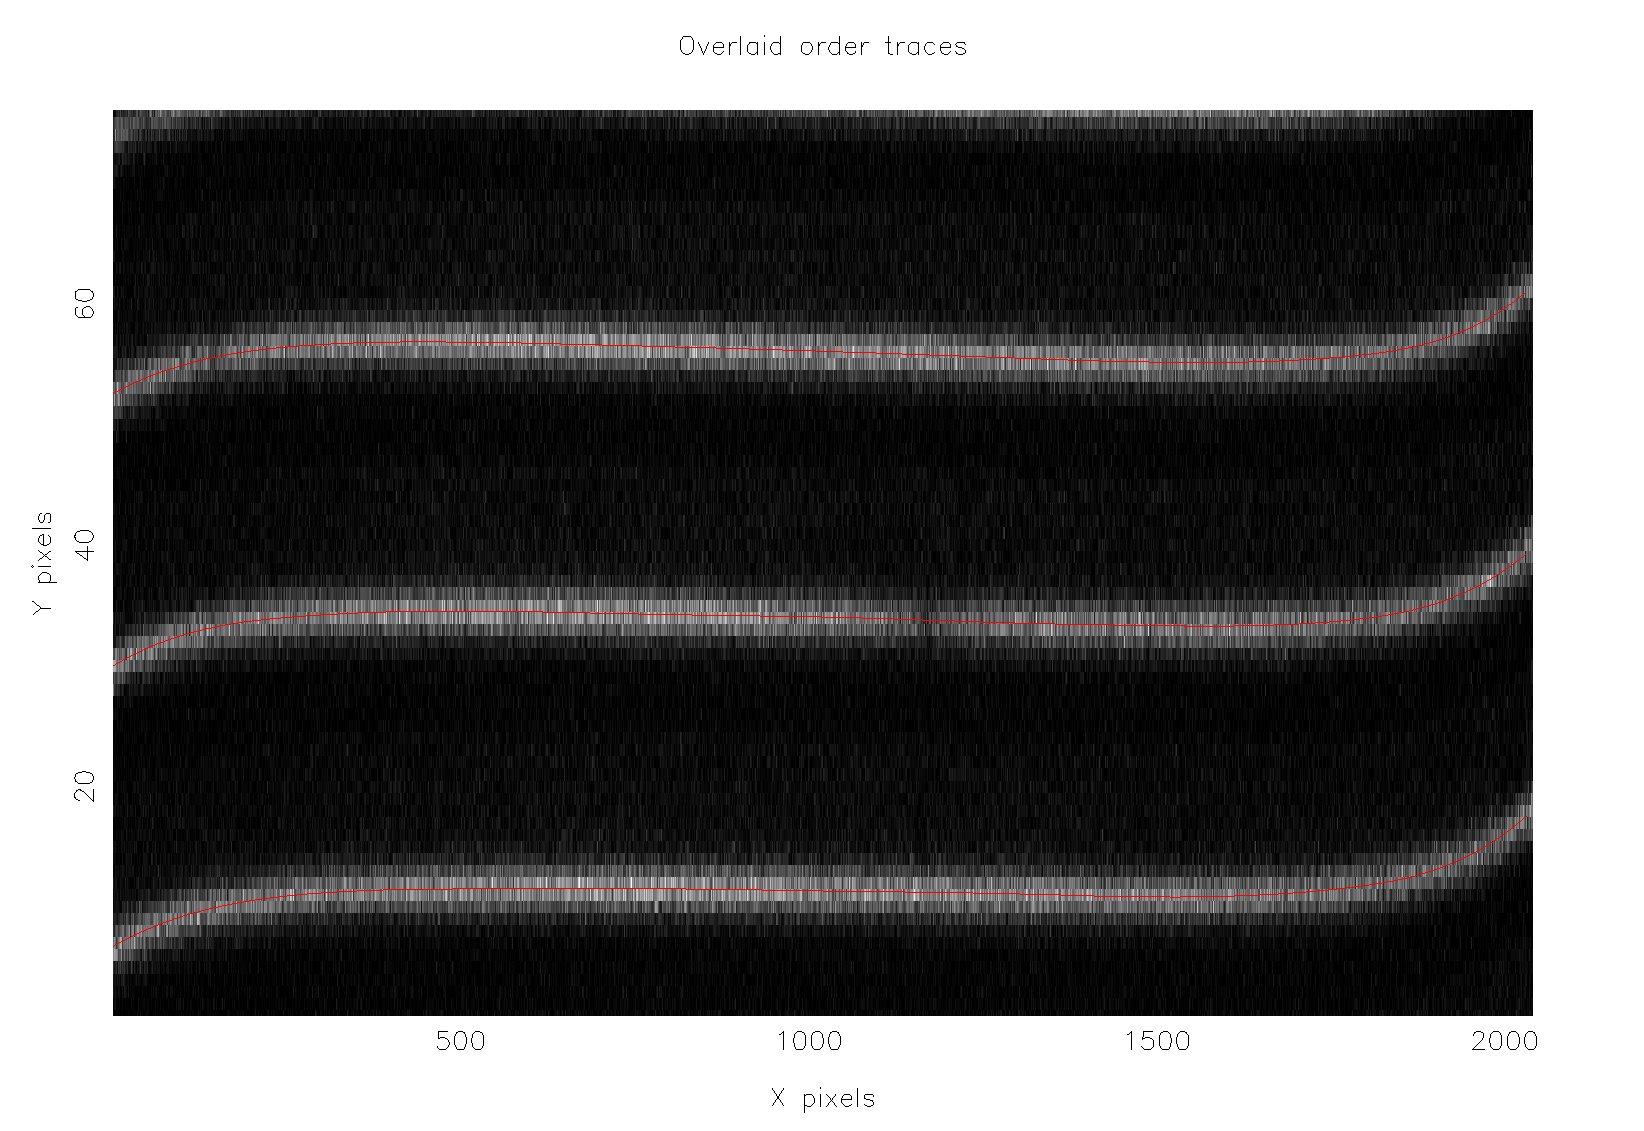
\includegraphics[width=\textwidth]{sun152_cover}

\parbox{140mm}{
\caption{A typical set of order paths as plotted using ECHMENU Option~15.
The distortions at the order extremities are due to the IPCS detector used.}
\label{fi_order}
}
\end{center}
\end{figure}

\echpars{
\epar{TRACIM}{Frame for order tracing.}{TRACIM}
\epar{TUNE\_DIAGNOSE}{YES to log activity to debugging file.}{TUNE_DIAGNOSE}
\lepar{TUNE\_MAXPOLY}{Maximum coefficients for fits.}{TUNE_MAXPOLY}
}

\echtask{option16}{ech_trcsis}{16:{\tt ech\_trcsis}}{Check Trace Consistency}
\myindex{Order!traces consistency check}
\myindex{Trace!consistency}

This option may be used to check the consistency of the order traces with
each other. The task predicts the path of each trace by fitting a function
to the positions of the other orders at each X-position.

The order whose trace deviates the most from the prediction is flagged as
the `worst' and the option to update the path using the predictions is
offered. This will allow the easy correction of common tracing problems
which can occur at the frame edges and with very faint or partial orders.

\indexcmdname{TUNE_CNSDEV}
\indexcmdname{TUNE_TRCNS}
In general it will only be effective when there are more than half a dozen
orders in the frame. The degree of variation and the consistency threshold
may be set using the parameters \htmlref{{\tt TUNE\_CNSDEV}}{par_TUNE_CNSDEV}
and \htmlref{{\tt TUNE\_TRCNS}}{par_TUNE_TRCNS}\@.

\echpars{
\epar{TRACIM}{Frame for order tracing.}{TRACIM}
\epar{TRC\_INTERACT}{YES for interactive order-fitting.}{TRC_INTERACT}
\epar{TRC\_NPOLY}{Number of coeffs of trace-fit function.}{TRC_NPOLY}
\epar{TUNE\_CNSDEV}{Maximum consistent deviation.}{TUNE_CNSDEV}
\epar{TUNE\_DIAGNOSE}{YES to log activity to debugging file.}{TUNE_DIAGNOSE}
\epar{TUNE\_MAXPOLY}{Maximum coefficients for fits.}{TUNE_MAXPOLY}
\epar{TUNE\_MXSMP}{Maximum number of X-samples to trace.}{TUNE_MXSMP}
\lepar{TUNE\_TRCNS}{Consistency requirement.}{TUNE_TRCNS}
}

\echredobj{
\eobj{NO\_OF\_ORDERS}{\_INTEGER}{READ}
\eobj{NX\_PIXELS}{\_INTEGER}{READ}
\eobj{NY\_PIXELS}{\_INTEGER}{READ}
\leobj{TRC\_POLY}{\_DOUBLE}{READ/WRITE}
}


\echtask{option17}{ech_decos2}{17:{\tt ech\_decos2}}{Post-trace Cosmic-Ray
  Locate}
\myindex{Cosmic rays!post-trace location}

This utility option should be run immediately after
\htmlref{{\tt ech\_spatial}/ECHMENU Option~4}{ech_spatial}
has been used to define the dekker and  object limits.

It uses information about the order paths and the spatial profile in order
to do a more effective cosmic-ray location. The sky and object pixels are
processed separately in two passes.

Each order in turn is processed by evaluating the degree to which its
pixels exceed their expected intensities (based upon profile and total
intensity in the increment).

A cumulative distribution function is then constructed and clipped at a
pre-determined sigma level. Clipping and re-fitting continues until a
Kolmogorov-Smirnov test indicates convergence or until the number of
clipped points falls to one per iteration.
\myindex{Data quality}
\myindex{Quality array}
Located cosmic-ray pixels are flagged in the quality array. Both this and
the pre-trace-locator are automatically followed by a routine to do
sky-line checking. This routine can restore any pixels it judges to be
possible sky line pixels (rather than cosmic-ray hits).
\myindex{Cosmic rays!coincidence checking}
If there are many frames of the same object available then it is possible
to use coincidence checking to enhance cosmic-ray detection. The script
{\tt decos\_many} will take list of input frames and perform this checking,
and flags the cosmic-ray pixels in each frame.  To use it type:

\begin{terminalv}
% $ECHOMOP_EXEC/decos_many
\end{terminalv}

\echpars{
\epar{INPTIM}{Frame to extract data from.}{INPTIM}
\epar{TUNE\_DIAGNOSE}{YES to log activity to debugging file.}{TUNE_DIAGNOSE}
\epar{TUNE\_DPRBTHR}{Maximum probability for K-S test.}{TUNE_DPRBTHR}
\epar{TUNE\_DSGMTHR}{Sigma threshold for clip.}{TUNE_DSGMTHR}
\epar{TUNE\_FINCPLY}{Number of coefficients.}{TUNE_FINCPLY}
\epar{TUNE\_MAXPOLY}{Maximum coefficients for fits.}{TUNE_MAXPOLY}
\epar{TUNE\_MINCR}{Minimum Cosmic-Ray intensity.}{TUNE_MINCR}
\lepar{TUNE\_MXSKYPIX}{Maximum number of sky pixels.}{TUNE_MXSKYPIX}
}


\echredobj{
\eobj{DEK\_ABOVE}{\_INTEGER}{READ}
\eobj{DEK\_BELOW}{\_INTEGER}{READ}
\eobj{NO\_OF\_ORDERS}{\_INTEGER}{READ}
\eobj{NX\_PIXELS}{\_INTEGER}{READ}
\eobj{NY\_PIXELS}{\_INTEGER}{READ}
\eobj{OBJ\_MASK}{\_INTEGER}{READ}
\eobj{SKY\_MASK}{\_INTEGER}{READ}
\eobj{SKY\_SPECTRUM}{\_REAL}{READ/WRITE}
\leobj{TRC\_POLY}{\_DOUBLE}{READ}
}


\echtask{option18}{ech_decimg}{18:{\tt ech\_decimg}}{Image Cosmic-Ray Pixels}
\myindex{Cosmic rays!imaging}

This option uses the quality array to determine which pixels have been
flagged as contaminated by cosmic-ray hits. It then takes the original
object frame and makes a copy in which all the hit pixels are replaced by
zero values. This frame should then be blinked with the original to
visually assess the success of the cosmic-ray location process.

\echpars{
\epar{INPTIM}{Frame to extract data from.}{INPTIM}
\epar{OUTPUT\_IMAGE}{Output image frame.}{OUTPUT_IMAGE}
\epar{TRACIM}{Frame for order tracing.}{TRACIM}
\lepar{TUNE\_DIAGNOSE}{YES to log activity to debugging file.}{TUNE_DIAGNOSE}
}

\echtask{option19}{ech_qextr}{19:{\tt ech\_qextr}}{Quick-look Extraction}
\myindex{Quick-look extraction}
\myindex{Extraction!quick-look}

This option allows quick extraction of an order (or all orders) once
\htmlref{{\tt ech\_spatial}/ECHMENU Option~4}{ech_spatial}
has been completed (object- and sky-pixel selection). The
extraction method used is simple sum of pixels in the dekker and the sky
subtraction is done by calculating the average value over all sky pixels in
the increment. No flat-field balance factors are used. This option should
only be used to get a quick-look at the data, the spectra produced should
not be used for further analysis as much better results will be obtained by
using Option~8 for a full extraction.

\echpars{
\epar{ARC}{Name(s) of reference (arc) lamp image(s).}{ARC}
\epar{INPTIM}{Frame to extract data from.}{INPTIM}
\epar{PHOTON\_TO\_ADU}{Conversion factor for photons.}{PHOTON_TO_ADU}
\epar{READOUT\_NOISE}{Detector readout noise in counts.}{READOUT_NOISE}
\epar{TUNE\_DIAGNOSE}{YES to log activity to debugging file.}{TUNE_DIAGNOSE}
\epar{TUNE\_MAXPOLY}{Maximum coefficients for fits.}{TUNE_MAXPOLY}
\epar{TUNE\_MXSKYPIX}{Maximum number of sky-pixels.}{TUNE_MXSKYPIX}
\lepar{TUNE\_NOARC}{YES if no arc frame is available.}{TUNE_NOARC}
}


\echredobj{
\eobj{DEK\_ABOVE}{\_INTEGER}{READ}
\eobj{DEK\_BELOW}{\_INTEGER}{READ}
\eobj{EXTRACTED\_ARC}{\_REAL}{READ/WRITE}
\eobj{EXTRACTED\_OBJ}{\_REAL}{READ/WRITE}
\eobj{EXTR\_ARC\_VAR}{\_REAL}{READ/WRITE}
\eobj{EXTR\_OBJ\_VAR}{\_REAL}{READ/WRITE}
\eobj{NO\_OF\_ORDERS}{\_INTEGER}{READ}
\eobj{NX\_PIXELS}{\_INTEGER}{READ}
\eobj{NY\_PIXELS}{\_INTEGER}{READ}
\eobj{OBJ\_MASK}{\_INTEGER}{READ}
\eobj{SKY\_MASK}{\_INTEGER}{READ}
\leobj{TRC\_POLY}{\_DOUBLE}{READ}
}


\echtask{option20}{ech_wvcsis}{20:{\tt ech\_wvcsis}}{Check Wavelength Scales}
\myindex{Wavelength scales!consistency check}

This function performs a function analogous to that performed by
\htmlref{Option~16}{ech_trcsis}
(order traces), only operating upon the wavelength fits.

It is thus used after \htmlref{Option~10}{ech_idwave} has been used
to calculate the wavelength scales.

The wavelength consistency check is confined to those areas beyond the
range within which lines have been identified. It therefore only corrects
the very ends of the orders wavelength scales.

These are the regions where problems are most likely to occur,  as the
polynomial fits can become unstable when a high number of coefficients has
been used, and there are no fitted points for a substantial fraction of the
order ({\it{e.g.}}, first 20\%).

\echpars{
\epar{AUTO\_ID}{YES for fully automatic identification.}{AUTO_ID}
\epar{ECH\_FTRDB}{Reference line list database.}{ECH_FTRDB}
\epar{TUNE\_DIAGNOSE}{YES to log activity to debugging file.}{TUNE_DIAGNOSE}
\epar{TUNE\_MAXPOLY}{Maximum coefficients for fits.}{TUNE_MAXPOLY}
\epar{TUNE\_MAXRFLN}{Maximum number of reference lines.}{TUNE_MAXRFLN}
\epar{TUNE\_MXSMP}{Maximum number of X-samples to trace.}{TUNE_MXSMP}
\lepar{W\_NPOLY}{Number of coeffs of wavelength fitting function.}{W_NPOLY}
}


\echredobj{
\eobj{EFTRDB\_WAVELENGT}{\_REAL}{READ}
\eobj{ID\_COUNT}{\_INTEGER}{READ/WRITE}
\eobj{ID\_LINES}{\_REAL}{READ/WRITE}
\eobj{ID\_STATUS}{\_INTEGER}{READ/WRITE}
\eobj{ID\_WAVES}{\_REAL}{READ/WRITE}
\eobj{NO\_OF\_ORDERS}{\_INTEGER}{READ}
\eobj{NX\_PIXELS}{\_INTEGER}{READ}
\eobj{OBS\_INTEN}{\_REAL}{READ}
\eobj{OBS\_LINES}{\_REAL}{READ}
\eobj{ORDER\_IDNUM}{\_INTEGER}{READ}
\eobj{WSEAR\_END}{\_REAL}{READ}
\eobj{WSEAR\_START}{\_REAL}{READ}
\leobj{W\_POLY}{\_DOUBLE}{READ/WRITE}
}


\echtask{option21}{ech_mulmrg}{21:{\tt ech\_mulmrg}}{Merge Multiple Spectra}
\myindex{Merge multiple spectra}
\myindex{Multiple object frames}

This utility option is provided to assist in co-adding spectra from many
frames together. This option assumes that the first frame in the reduction
has been scrunched with the required wavelength scale.

It then reads a list of additional reduction database names from an
ASCII file called {\tt NAMES.LIS}. The extracted spectra from each of these
reduction files is then scrunched to the same scale and co-added into the
scrunched spectra in the current reduction file.

The parameter \htmlref{{\tt TUNE\_MRGWGHT}}{par_TUNE_MRGWGHT}
\indexcmdname{TUNE_MRGWGHT} controls the type of weighting used during addition.

\echpars{
\epar{SET\_WSCALE}{YES to scrunch to a global bin size.}{SET_WSCALE}
\epar{TUNE\_AIRTOVAC}{YES to correct wavelengths.}{TUNE_AIRTOVAC}
\epar{TUNE\_DIAGNOSE}{YES to log activity to debugging file.}{TUNE_DIAGNOSE}
\epar{TUNE\_FLUX}{YES if flux is to be conserved.}{TUNE_FLUX}
\epar{TUNE\_INTR}{YES if linear interpolation required.}{TUNE_INTR}
\epar{TUNE\_LOG}{YES if output scale logarithmic.}{TUNE_LOG}
\epar{TUNE\_MAXPOLY}{Maximum coefficients for fits.}{TUNE_MAXPOLY}
\epar{TUNE\_MRGMAXX}{Number of rhs pixels to ignore.}{TUNE_MRGMAXX}
\epar{TUNE\_MRGMINX}{Number of lhs pixels to ignore.}{TUNE_MRGMINX}
\epar{TUNE\_MRGWGHT}{Type of weighting to apply.}{TUNE_MRGWGHT}
\epar{TUNE\_QUAD}{YES if quadratic interpolation required.}{TUNE_QUAD}
\epar{TUNE\_SCFRACT}{Fractional ratio for twin scales.}{TUNE_SCFRACT}
\epar{TUNE\_SCRADD}{Number of bins to add together.}{TUNE_SCRADD}
\epar{TUNE\_SCRMODE}{Scrunching mode control.}{TUNE_SCRMODE}
\lepar{TUNE\_SKEW}{Skew shift in bins.}{TUNE_SKEW}
}


\echredobj{
\eobj{ERR\_SPECTRUM}{\_REAL}{READ/WRITE}
\eobj{EXTRACTED\_OBJ}{\_REAL}{READ}
\eobj{EXTR\_OBJ\_VAR}{\_REAL}{READ}
\eobj{NO\_OF\_BINS}{\_INTEGER}{READ}
\eobj{NO\_OF\_ORDERS}{\_INTEGER}{READ}
\eobj{NREF\_FRAME}{\_INTEGER}{READ}
\eobj{NX\_PIXELS}{\_INTEGER}{READ}
\eobj{NX\_REBIN}{\_INTEGER}{READ}
\eobj{SCRNCHD\_OBJ}{\_REAL}{READ/WRITE}
\eobj{SCRNCHD\_OBJV}{\_REAL}{READ/WRITE}
\eobj{SCRNCHD\_WAVES}{\_DOUBLE}{READ/WRITE}
\eobj{WAVELENGTH}{\_DOUBLE}{READ/WRITE}
\eobj{W\_POLY}{\_DOUBLE}{READ}
\leobj{1D\_SPECTRUM}{\_REAL}{READ/WRITE}
}


\echtask{option22}{ech_mdlbck}{22:{\tt ech\_mdlbck}}{Model Scattered Light}

This option is used in place of Option~6 (Model sky) in cases where there
is severe scattered light contamination. It works by fitting independent
polynomials/splines to each image column (actually only the inter-order
pixels). Once the column fits have been done the results are used as input
to a second round of fits which proceeds parallel to the the order traces.

The final fitted values are saved in the sky model arrays.

This process is very CPU intensive and should not be used unless is it
needed.

\echpars{
\epar{FFIELD}{Name of flat-field image.}{FFIELD}
\epar{INPTIM}{Frame to extract data from.}{INPTIM}
\epar{PHOTON\_TO\_ADU}{Conversion factor for photons.}{PHOTON_TO_ADU}
\epar{READOUT\_NOISE}{Detector readout noise in counts.}{READOUT_NOISE}
\epar{SKYFIT}{Function for sky fitting.}{SKYFIT}
\epar{TUNE\_DIAGNOSE}{YES to log activity to debugging file.}{TUNE_DIAGNOSE}
\epar{TUNE\_MAXPOLY}{Maximum coefficients for fits.}{TUNE_MAXPOLY}
\epar{TUNE\_MXSKYPIX}{Maximum number of sky-pixels.}{TUNE_MXSKYPIX}
\epar{TUNE\_NOFLAT}{YES if no flat-field frame is available.}{TUNE_NOFLAT}
\epar{TUNE\_SKYPOLY}{Degree of polynomial to use for sky.}{TUNE_SKYPOLY}
%\epar{TUNE\_SKYLTHR}{Sigma threshold for sky-lines.}{TUNE_SKYLTHR}
\epar{TUNE\_SKYREJ}{Number of reject cycles.}{TUNE_SKYREJ}
\epar{TUNE\_SKYRTHR}{Reject threshold in sigma.}{TUNE_SKYRTHR}
\lepar{TUNE\_SKYSIM}{YES for sky simulation to be used.}{TUNE_SKYSIM}
}

\echredobj{
\eobj{DEK\_ABOVE}{\_INTEGER}{READ}
\eobj{DEK\_BELOW}{\_INTEGER}{READ}
\eobj{FITTED\_FLAT}{\_REAL}{READ}
\eobj{FITTED\_SKY}{\_REAL}{READ/WRITE}
\eobj{FLAT\_ERRORS}{\_REAL}{READ}
\eobj{FSKY\_ERRORS}{\_REAL}{READ/WRITE}
\eobj{NO\_OF\_ORDERS}{\_INTEGER}{READ}
\eobj{NX\_PIXELS}{\_INTEGER}{READ}
\eobj{NY\_PIXELS}{\_INTEGER}{READ}
\eobj{SKY\_MASK}{\_INTEGER}{READ}
\eobj{SKY\_SPECTRUM}{\_REAL}{READ/WRITE}
\eobj{SKY\_VARIANCE}{\_REAL}{READ/WRITE}
\leobj{TRC\_POLY}{\_DOUBLE}{READ}
}


\echtask{option23}{ech_tuner}{23:{\tt ech\_tuner}}{Adjust Tuning Parameters}
\myindex{Tuning parameters!edit}
\myindex{Hidden parameters!edit}
\myindex{Parameters!edit tuning}

This option simply provides a centralised mechanism for viewing and editing
the values of all the tuning parameters known to the system.

Most of the time it is more convenient to use the -option syntax from the
main menu, as this only lists parameters used by the current default
option.

In Option~23, any parameters used by the current default option are flagged
with an asterix.

If, when used, a tuning parameter has a non-default value, an informational
message is displayed.


\echtask{option24}{ech_single}{24:{\tt ech\_single}}{Set Single-order
  Processing}
\myindex{Order!process single}

Allows the selection of a single order for all tasks which operate on an
order-by-order basis, {\it{e.g.}}, to re-fit the order trace for order 3,
leaving all other orders unchanged, you would first use this option to
change the selected order to number 3, and then invoke the
\htmlref{{\tt ech\_fitord} task/ECHMENU Option~3}{ech_fitord}.

Note that any options which operate on all orders at once ({\it{e.g.}},
trace consistency checking) will still operate correctly when a single
order is selected, as they ignore the selection and use all the orders
anyway).

Note that when using the individual tasks the strategy for selecting single
order/all order operation is different. Individual function tasks which can
operate on single orders all utilise the parameter {\tt
IDX\_NUM\_ORDERS}\@.

which you should set to the number of the order to process, or to zero to
indicate that all orders are to be processed in turn. {\it{e.g.}}:

\begin{terminalv}
% ech_trace idx_num_orders=4
\end{terminalv}

would just trace order number 4.

\echtask{option25}{ech_all}{25:{\tt ech\_all}}{Set All-order Processing}
\myindex{All order processing}

Selects automatic looping through all available orders for all tasks which
are performed on an order by order basis.  This is the default method of
operation.


\echtask{option26}{ech_disable}{26:{\tt ech\_disable}}{Disable an Order}
\myindex{Disable order}
\myindex{Ignore order}
\myindex{Delete order}

This option disables an order from any further processing. The mechanism
for doing this is to remove the order trace. If you need to re-enable an
order then it should be re-traced by using \htmlref{Option~24}{option24}
(select single order) and then \htmlref{Option~2}{ech_trace}
(trace an order).

\echpars{
\epar{BAD\_ORDER}{Number of the order to disable.}{BAD_ORDER}
\epar{TUNE\_DIAGNOSE}{YES to log activity to debugging file.}{TUNE_DIAGNOSE}
\lepar{TUNE\_MAXPOLY}{Maximum coefficients for fits.}{TUNE_MAXPOLY}
}

\echtask{option27}{ech_plot}{27:{\tt ech\_plot}}{Run Plot Utility}
\myindex{Graphics!plot utility}
\myindex{Plotter}

Many of the temporary results arrays stored in the reduction database can
be of assistance when tracking down problems during a reduction. All of
these can be graphically examined using the \verb+ech_plot+ task/ECHMENU
Option~27.

This utility prompts for object names for the Y-axis (and optionally the
X-axis separated by a comma). If a null object name is returned then that
axis will be automatically generated using monotonically increasing integer
values.

The normal usage will be to supply only the name of the Y-axis object and
leave the X-axis to be auto generated. An exception is when plotting
wavelength objects along the X-axis.

Note that unless you are interested in  the first order of a multi-order
array then the array indices to start plotting from {\bf must} be supplied.

{\it{e.g.}}: OBJ would denote the first orders' extracted object spectra.
OBJ[1,4] would denote the fourth orders' extracted object spectra.
ARC[100,13,2] would denote the region of the second arc frames thirteenth
order starting at X-sample 100.

Note that in this last case unless the N(umber) of samples to plot has been
set to less than the array X-dimension then some samples from the
fourteenth order would also be plotted.

Also provided are the following facilities most of which are selected by
typing the single character followed by carriage-return.

\begin{itemize}

\item {\sunspec{\Large\tt}{\bf} B}(rowse)
     \myindex{FIGARO!IMAGE}
     \myindex{Plotter!image browse}
     Used in conjunction with an imaging display.
     The object or arc data frame should be specified or it will be
     prompted for ({\it{e.g.}}:  B MYOBJ)

     {\sc echomop} will display the image and then put a cursor on the display,
     you can then position the cursor and type a key indicating which type of
     data you wish to select for plotting.

     Options include:

     \begin{itemize}

     \item {O --- for object order}
     \item {A --- for arc order}
     \item {S --- for scrunched object order}
     \item {F --- for flat-field model balance factors}
     \item {S --- for sky model}

     \end{itemize}

     All arrays are plotted using the cursor position to determine which
     order, subsample {\it etc.} is required. By default the full X-axis
     dimension is used, unless the N command is used to explicitly set the
     number of samples to plot.

     For example, setting N to 20 and imaging the arc frame would allow
     the extracted profile of an arc line to be plotted simply by
     positioning the cursor on the line on the image and hitting A,
     plotting a 20-sample section of the extracted arc from the requisite
     order.

\item {\sunspec{\Large\tt}{\bf} D}(irectory)/
      {\sunspec{\Large\tt}{\bf} FD} (full directory)
     \myindex{Plotter!known objects}

     Lists a directory of reduction database
     objects. These are not all arrays and therefore not all plottable.
     The most common objects are listed by D(ir) and are all arrays.

     The names are such that it is easy to recognise which arrays contain
     the information required. For example the object FFLT contains the
     fitted flat-field balance factors for each order and trace offset.

     Specifying an object name without any dimensional specifications will
     plot the first N elements starting from the beginning of the array,
     {\it{i.e.}}, ARRAY[1,1,1....] to ARRAY[N,1,1....]

\item {\sunspec{\Large\tt}{\bf} E}(xit)

     Returns to the main ECHMENU menu or exits from
     the \verb+ech_plot+ single activity task.

\item {\sunspec{\Large\tt}{\bf} G}(raphics/Grayscale)

     Toggles the plotting mode. The
     grayscale mode is useful for plotting swathes of 2-D and 3-D objects.
     {\it{e.g.}}:

     \begin{itemize}

     \item in Graphics mode --- FSKY[1,1,1] plots the first spatial
            increment of the sky model for order 1.

     \item in Grayscale mode --- FSKY[1,1,1] images the entire sky model
            for order 1.  Thus in most cases the first two indices will
            always be equal to 1 when using grayscale plotting.

     \end{itemize}

\item {\sunspec{\Large\tt}{\bf} H}(elp)

     Accesses the HELP Facility.

\item {\sunspec{\Large\tt}{\bf} I}(nteractive cursor)

     Sets the cursor display such that
     the cursor may be moved around the next graph to be plotted and the
     exact data values plotted can be examined (by pressing the space
     character).

\item {\sunspec{\Large\tt}{\bf} N}(umber of samples)
     \myindex{Plotter!subsets}

     Sets the number of data samples plotted from the arrays.
     Unless specified in the object name,
     plotting always commences from the beginning of the array and the N
     is set to the maximum number of elements in the array. Setting a
     smaller value effectively allows you to zoom in on a small subsection
     of any array.

\item {\sunspec{\Large\tt}{\bf} L}(imit setting)
     \myindex{Plotter!set limits}

     Allows the X- and Y-limits of the plot to be set.
     The limits are normally calculated automatically
     according to the data in the array. To resume auto scaling just set
     all the X,Y limits back to 0.

\item{\sunspec{\Large\tt}{\bf} R}(ebin factor)
     \myindex{Plotter!rebinning}
     \myindex{Re-binning!using plotter}

     Sets the degree of re-binning to be
     performed on the data before plotting it. It remains active until
     reset to 1 (indicating no rebinning). Specify a positive factor for
     simple summed bins, and a negative factor to request full smoothing.

\item{\sunspec{\Large\tt}{\bf} S}(tyle)
     \myindex{Plot styles}

     Allows the specification of various style
     parameters for the plots. The line styles and colours may be
     specified, as may the plot style. The following keywords are
     recognised and may be appended to the S to save time. {\it{e.g.}},
     \verb+S RED+ sets the plot colour to red.

     Keywords:

     \begin{itemize}

     \item {Colours} RED,WHITE,BLACK,BLUE,GREEN,YELLOW,CYAN,MAGENTA
     \item {Line types} DOTD,DASH,LINE
     \item {Plot types} POINTS,LINES,*,+,x,BINS
     \item {Text fonts} ROMAN,ITALIC
     \item {Misc} PROMPT,NOPROMPT

     \end{itemize}

\item{\sunspec{\Large\tt}{\bf} U}(ser-defined window)
     \myindex{Graphics!multiple per screen}

     Toggles user-windowing.
     When this is activated each subsequent plot will prompt the user to select
     two limits on the display surface. A box based on these limits will then
     be used for the plot.

     This allows complete freedom in producing a set of plots. Plots may
     be partially overlaid, stacked {\it etc.} Once you have produced the
     display required the easiest way to get a hardcopy of it is to use
     the built in facilities on your workstation/X-terminal to grab it
     from the screen (this normally results in a Postscript file).

\item{\sunspec{\Large\tt}{\bf} W}(indowing)

     Permits the division of the plotting surface
     into panes into which subsequent graphs are plotted. Two factors are
     requested, the subdivision factor in the horizontal, and in the
     vertical directions. {\it{e.g.}}, 3 and 2 would divide the surface
     into two rows of three graphs. Setting both factors to 1 restores
     normal single graph behaviour.

\item{\sunspec{\Large\tt}{\bf} +} (Overplot)
     \myindex{Overlaying graphs}
     \myindex{Plotter!overlaying}

     May be used either on its own or be used as a prefix to any object name.
     Causes the next graph to be plotted over the previous one without
     re-drawing the axes {\it etc.}

\item{\sunspec{\Large \tt}{\bf} ?} (Help)

     The same as H(elp).

\item{Name of object(s) to plot}

     A single object name indicates that the object array is to be plotted
     along the Y-axis using a default linear scale as the X-axis.

     Two object names separated by a comma indicates that the two arrays
     are to be plotted against each other.

\end{itemize}


\echtask{option28}{ech_menu}{28:{\tt ech\_menu}}{Display Full Menu}

This option selects the display of the full menu of options available in
ECHMENU top-level menu. By default only the utility options and the
currently most likely selections will appear on the menu.


\echtask{option29}{ech_system}{29:{\tt ech\_system}}{Do System Command}
\myindex{System commands}
\myindex{Spawning a subprocess}

This option allows the execution of one or more system level commands
without leaving and re-starting the ECHMENU shell task.

The command is prompted for with:

\begin{terminalv}
- System_$ /''/ >
\end{terminalv}

you should then enter a command.  If more than one command is
required then the \verb+csh+ command should be given to initiate a fully
independent process.

This process must be terminated by a CTRL-D in order to return to the
ECHMENU shell task.
\myindex{ADAM!from spawned process}
This option can be used to perform system commands like \verb+ls+ and also
\xref{{\sc figaro}}{sun86}{} commands such as
\xref{IMAGE}{sun86}{IMAGE} {\it etc.}  However, {\sc echomop}
commands which change parameter values will not operate perfectly because the
monolith already has the {\sc echomop} parameter file open.

System commands can also be entered directly at the Option: prompt by
making the first character a {\tt \$}. Thus:

\begin{terminalv}
$ls
\end{terminalv}

would execute the system `directory' command, and return to the main menu.

\echtask{option30}{ech_genflat}{30:{\tt ech\_genflat}}{Output Flattened-field}

\begin{figure}
\begin{center}
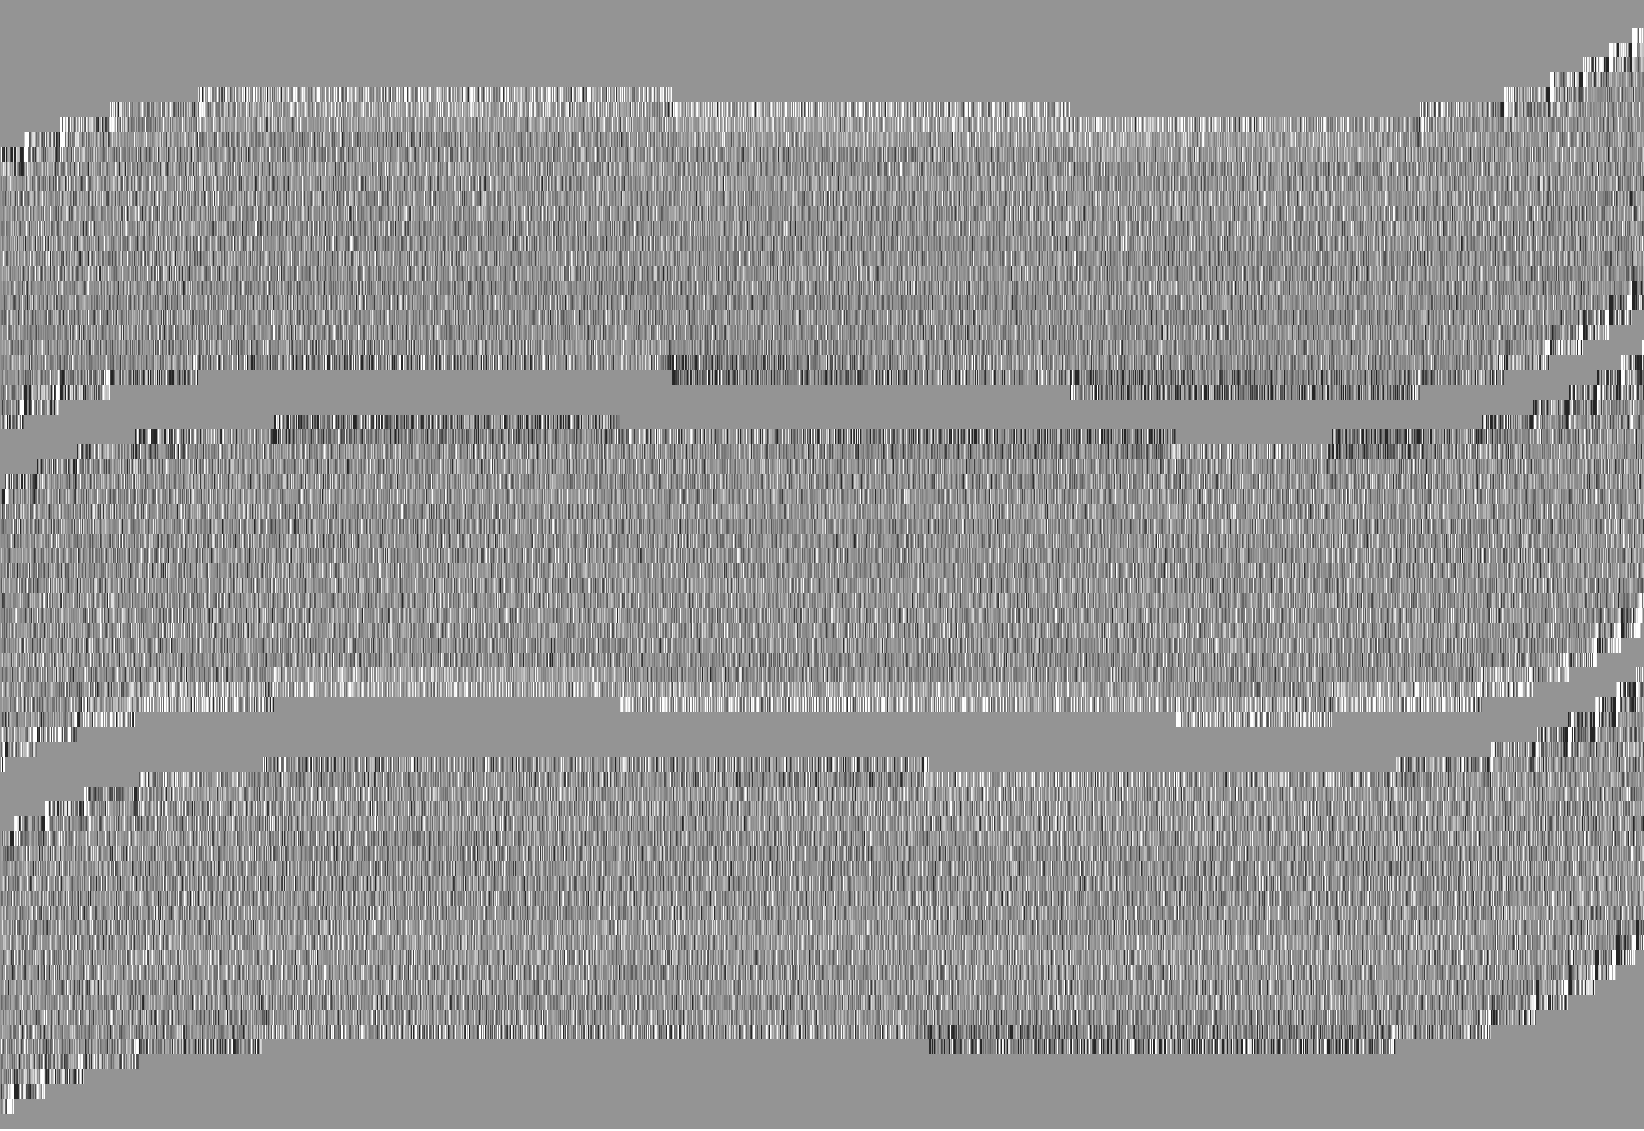
\includegraphics[width=\textwidth]{sun152_08}

\parbox{140mm}{
\caption{A flattened-field.  This was produced using ECHMENU Option 30.}
\label{fi_genflat}
}
\end{center}
\end{figure}

This option was introduced at {\sc echomop} version 3.2-0.  The flat-field balance
factors produced by \htmlref{{\tt ech\_ffield}}{ech_ffield} are written to an
image which can then be inspected, for example using \xref{{\sc kappa}}{sun95}{}
\xref{DISPLAY}{sun95}{DISPLAY}.

\echpars{
\epar{ECH\_RDUCD}{Output spectrum data file.}{ECH_RDUCD}
\epar{TUNE\_DIAGNOSE}{YES to log activity to debugging file.}{TUNE_DIAGNOSE}
\epar{TUNE\_MAXPOLY}{Maximum coefficients for fits.}{TUNE_MAXPOLY}
\epar{TUNE\_MXSKYPIX}{Maximum number of sky pixels.}{TUNE_MXSKYPIX}
\lepar{TUNE\_NOFLAT}{YES if no flat-field frame is available.}{TUNE_NOFLAT}
}

\vspace*{11mm}

\echtask{option31}{ech_exit}{31:{\tt ech\_exit}}{Exit ECHMENU}
\myindex{Exit}
\myindex{Closedown}

This option exits the ECHMENU shell task.  It is also possible to select
this option by typing either EXIT, QUIT, a single `E' or `Q', or 99,
followed by carriage return.


%%%%%%%%%%%%%%%%%%%%%%%%%%%%%%%%%%%%%%%%%%%%%%%%%%%%%%%%%%%%%%%%%%%%%%%%%%%
\section{\mlabel{parameters}PARAMETERS}

This is a complete list of all the parameters used by {\sc echomop} tasks.

\sunspec{\begin{description}}{}

\echparameter{ARC}{ARC}{
 \_CHAR
}{
 The names of all reference images to be used for wavelength
 calibration must be supplied here.  The number of images should be
 equivalent to the number specified for parameter {\tt NREF\_FRAME}. The
 image names should be separated by commas, for example: {\tt
 reffrm1, reffrm2}.

 Note that in most circumstances there will only be two reference
 frames.  One taken prior to the object frame, and one subsequently.
 If you do not wish to provide an arc frame at all then you may reply
 \texttt{NONE} is response to this prompt or, alternatively set the
 parameter \htmlref{{\tt TUNE\_NOARC=YES}}{par_TUNE_NOARC}.
 If no arc is available then you
 must provide your own sets of wavelength feature positions, or
 wavelength scales, {\bf if} wavelength calibration is required.
}

\echparameter{ARC\_TYPE}{ARC_TYPE}{
 \_CHAR
}{
 {\sl As of {\sc echomop} v3.3-0, this parameter is ignored and should
  be removed from any scripts using it.  The reference-line
  database should be specified by the parameter
  \htmlref{{\tt ECH\_FTRDB}}{par_ECH_FTRDB}. The parameter will
  be completely removed at the next release of {\sc echomop}.}
}

\echparameter{ASCII\_FILE}{ASCII_FILE}{
 \_CHAR
}{
 The name of the ASCII data file to be produced.

 The default is {\tt echomop\_output.txt}.
}

\echparameter{AUTO}{AUTO}{
 \_LOGICAL
}{
 If \texttt{AUTO=YES} then {\sc echomop} will use all the options available
 to automate the processes it invokes.  Currently the following
 parameters will be affected:

\begin{itemize}
\item {\tt TRC\_INTERACT}     set to \texttt{NO}.
\item {\tt TRC\_VETO}         set to \texttt{NO}.
\item {\tt ID\_INTERACTIVE}   set to \texttt{NO}.
\item {\tt CR\_INTER}         set to \texttt{NO}.
\item {\tt 2D\_INTERACT}      set to \texttt{NO}.
\item {\tt PFL\_INTERACT}     set to \texttt{NO}.
\end{itemize}
}

\echparameter{AUTO\_ID}{AUTO_ID}{
 \_LOGICAL
}{
 Specifies that automation is required when arc line identification
 is being done.  Interactively, options are available to allow you
 to tune the fitted wavelength polynomial, add/delete features
 {\it etc.}  If {\tt AUTO\_ID} is set to \texttt{YES} then the package will
 try to identify
 the arc line features automatically.  For orders with sufficient
 features this will usually be successful ( $>$12 lines), and a useful
 strategy is probably to do an automatic run first, and then manually
 examine the fitted features to verify their suitability.
}

\echparameter{BAD\_ORDER}{BAD_ORDER}{
 \_INTEGER
}{
 Specifies an order which is to be disabled from further processing.

 The default value is zero which is ignored, in case of a mistake.

 Orders are disabled by writing the `bad value' quantity into the
 first coefficient of the trace polynomial.  This ensures that they
 also appear disabled to other tasks (almost all of which will need
 the trace polynomials).

 To re-enable an order, re-fit a polynomial to its traced path, using
 \htmlref{{\tt{ech\_fitord}}/echmenu option 3}{ech_fitord}.
}

\echparameter{BIN\_SIZE}{BIN_SIZE}{
 \_REAL
}{
 Specifies the bin size in wavelength units.  This bin size is only
 used when scrunching to a global wavelength scale.  By default the
 program will calculate an appropriate bin size for you, but this
 parameter allows you to override this by supplying a non-zero value.

 Initial suggested value: \texttt{0.0}.
}

\echparameter{BLZFIT}{BLZFIT}{
 \_CHAR
}{
 This parameter selects the type of line fit for blaze function
 fitting.

 The recognised functions are \texttt{POLY} (the default), \texttt{MEDIAN}
 and \texttt{SPLINE}.

 {\bf Note} that the required maximum number of coefficients is
 different in each case.  For \texttt{POLY} the maximum number of coefficients
 corresponds to the number of degrees plus one, so for a cubic use coeffs=4.
 For a \texttt{SPLINE} the maximum number of coefficients corresponds to
 \sunspec{(knots+7)$\times$2}{2x(knots+7)}, so for 3 knots use coeffs=20.
 If you are using
 \texttt{SPLINE} fits then you should ensure that the value of
 \htmlref{{\tt TUNE\_MAXPOLY}}{par_TUNE_MAXPOLY} is set accordingly, as
 well as using an appropriate value for
 \htmlref{{\tt BLZ\_NPOLY}}{par_BLZ_NPOLY}.

 When \texttt{MEDIAN} is selected local medians of X-extent
 \htmlref{{\tt BLZ\_NPOLY}}{par_BLZ_NPOLY}-pixels are used as the blaze
 function.

 Initial suggested value: \texttt{POLY}.
}

\echparameter{BLZ\_INTERACT}{BLZ_INTERACT}{
 \_LOGICAL
}{
 Set to \texttt{YES} if the blaze fitting is to be done interactively.
 Automatic fitting is performed otherwise.

 Initial suggested value: \texttt{NO}.
}

\echparameter{BLZ\_NPOLY}{BLZ_NPOLY}{
 \_INTEGER
}{
 The default number of coefficients to be used when fitting functions
 to the order blaze.

 The type of function to be used is set using the parameter
 \htmlref{\texttt{BLZFIT}}{par_BLZFIT}
 (default is \texttt{POLY} for polynomial).

 When \texttt{BLZFIT=POLY} then the number of coefficients should be set to
 degree of polynomial + 1.

 When \texttt{BLZFIT=SPLINE} the number of coefficients should be set to
 \sunspec{(number of knots + 7)$\times$2}{2 x (number of knots + 7)}.

 When \texttt{BLZFIT=MEDIAN} the number of coefficients should be set to the
 number of pixels over which a local median value of the blaze function
 is to be found.

 For example, setting {\tt BLZ\_NPOLY} to 4 would permit the fitting of
 polynomials of the form:

\sunspec{
 ${\rm constant} + ax + bx^{2} + cx^{3}$.
}{
\begin{terminalv}
constant + ax + bx squared + cx cubed
\end{terminalv}
}

 Initial suggested value: \texttt{7}.
}

\echparameter{CENTRAL\_ONUM}{CENTRAL_ONUM}{
 \_INTEGER
}{
 Parameter is `hidden'
}

\echparameter{CENTRAL\_WAVE}{CENTRAL_WAVE}{
 \_REAL
}{
 Parameter is `hidden'
}

\echparameter{CR\_OUTPUT}{CR_OUTPUT}{
 \_CHAR
}{
 The name of the output image containing a copy of the original
 with suspected cosmic-ray pixels replaced either by interpolation,
 or by flag values.
}

\echparameter{DECIMG}{DECIMG}{
 \_CHAR
}{
 The name of the raw image in which cosmic-ray-pixel detection is to
 be performed.

 Pixels may be either replaced with an interpolated value, or by a
 flag value.
}

\echparameter{DISPLAY}{DISPLAY}{
 \_LOGICAL
}{
 If {\tt DISPLAY=YES} is used, then an imaging device is assumed to be
 available and some programs in the package will overlay plots on
 the image to help illustrate their results.

 For example, the paths of the orders as fitted with polynomials will
 be overlaid on a part of the traced image.

 Initial suggested value: \texttt{NO}.
}

\echparameter{ECH\_ECHAR}{ECH_ECHAR}{
 \_CHAR
}{
 The name of the file to use to exchange data with the
 \xref{ECHARC}{sun86}{ECHARC} program.
}

\echparameter{ECH\_FTRDB}{ECH_FTRDB}{
 \_CHAR
}{
 The name of the file containing the reference line list database.

 The database is built from a \texttt{.ARC} file using the task
 {\tt ech\_ftrdb}.

 The database should have the same file name as the \texttt{.ARC} file used
 for its creation.  The default is to use {\tt \$ARCDIRS/THAR}.
 Note the use
 of the {\tt\$ARCDIRS} environment variable to specify the search path for
 arc databases.  This should normally be used as it searches in the
 normal {\sc figaro} order.  If you wish to specify a private database then
 the full pathname may be provided, e.g., \texttt{/mydisk/mydir/sub/ANARC}.

 If no arc database exists for the \texttt{.ARC} list you want to use then
 use the {\tt ech\_ftrdb} task to create a copy.  You might like to check
 to see if anyone local already has the database you need.

 Initial suggested value: {\tt '\$ARCDIRS/THAR'}.
}

\echparameter{ECH\_RDCTN}{ECH_RDCTN}{
 \_CHAR
}{
 The name of the file created to hold the data reduction history.

 This file will normally be created by the first {\sc echomop} task run.
 Any valid datafile name can be used.

 By default the file is created in the current directory.
}

\echparameter{ECH\_RDUCD}{ECH_RDUCD}{
 \_CHAR
}{
 The name of the file to save data to.
}

\echparameter{ECH\_STRUCT}{ECH_STRUCT}{
 \_CHAR
}{
 The name of the file containing the definition used to create a
 reduction database.
}

\echparameter{EXTRACT\_MODE}{EXTRACT_MODE}{
 \_CHAR
}{
 The type of extraction to perform.

 This may be one of the following:

 \begin{quote}
    {\tt O} --- Optimal (default).

    {\tt S} --- Simple.

    {\tt P} --- Profile weighted.
 \end{quote}
}

\echparameter{FFIELD}{FFIELD}{
 \_CHAR
}{
 The name of the flat-field frame.

 The package uses this frame to calculate balance factors on a
 per-pixel basis.  If a balance frame is already available, then the
 frame should be supplied instead of a flat field, and the parameter
 \htmlref{{\tt TUNE\_PREBAL}}{par_TUNE_PREBAL} should be set.

 If you do not wish to supply a flat field at all, then you may
 either reply \texttt{NONE} to this prompt (must be uppercase), or
 set the parameter \htmlref{{\tt TUNE\_NOFLAT=YES}}{par_TUNE_NOFLAT}\@.

 If no flat-field frame is supplied then the balance factors will be
 set to unity for all pixels.
}

\echparameter{FLAG}{FLAG}{
 \_REAL
}{
 If interpolation is not required, the suspected cosmic-ray pixels
 will be replaced using the supplied flag value.
}

\echparameter{FLTFIT}{FLTFIT}{
 \_CHAR
}{
 The type of fit to be used for flat-field modelling.

 The available functions are \texttt{MEAN} (the default), \texttt{POLY},
 \texttt{SPLINE}, \texttt{MEDIAN}, \texttt{SLOPE} and \texttt{SMOOTH}.

 All modes except \texttt{POLY} and \texttt{SPLINE} use local neighbourhoods
 delineated using a sample size (in pixels) defined by
 \htmlref{{\tt TUNE\_FFLSMP}}{par_TUNE_FFLSMP}.

 Note that the required maximum number of coefficients for \texttt{POLY} and
 \texttt{SPLINE} are different.  For \texttt{POLY}, the maximum number of
 coefficients corresponds to the number of degrees plus one, so for a cubic use
 coeffs=4.  For a \texttt{SPLINE} the maximum number of coefficients corresponds
 to \sunspec{(knots+7)$\times$2}{2x(knots+7)}, so for 3 knots use coeffs=20.
 If you are using \texttt{SPLINE}
 fits then you should ensure that the value of
 \htmlref{{\tt TUNE\_MAXPOLY}}{par_TUNE_MAXPOLY} is set
 accordingly, as well as using an appropriate value for
 \htmlref{{\tt TUNE\_FFNXPLY}}{par_TUNE_FFNXPLY}
 and/or \htmlref{{\tt TUNE\_FFNYPLY}}{par_TUNE_FFNYPLY}.

 Initial suggested value: \texttt{MEAN}.
}

\echparameter{FRAME\_CHECK}{FRAME_CHECK}{
 \_LOGICAL
}{
 Set {\tt FRAME\_CHECK} if the processed frames are to be checked for
 bad rows and columns.

 The trace frame is checked, and the other frames are assumed to have
 identical bad row and/or column features.
}

\echparameter{HARD}{HARD}{
 \_CHAR
}{
 If a value for {\tt HARD} is specified, the plot is written to a file
 in the format defined by the {\tt HARD} parameter.

 For example, {\tt ps\_l} would generate Landscape format PostScript files.
}

\echparameter{HELIO\_COR}{HELIO_COR}{
 \_REAL
}{
 The heliocentric correction is applied to the output
 wavelength-scale of any results files.

 Initial suggested value: \texttt{0.0}.
}

\echparameter{HI\_WAVE}{HI_WAVE}{
 \_REAL
}{
 The identification of lines proceeds faster for smaller search
 ranges.  Specify the highest wavelength covered by the spectrum.
 The units in which the wavelength is expressed must be the same as
 those used in the \texttt{.ARC} line list file.  This will normally be
 Angstroms but may be changed by supplying an appropriate \texttt{.ARC} file.
}

\echparameter{IDX\_NREF\_FRAME}{IDX_NREF_FRAME}{
 \_INTEGER
}{
 Specifies the number of the arc frame to be processed.

 {\tt IDX\_} parameters provide a method of indexing reduction database
 arrays by order number and frame number.

 A non-zero value for {\tt IDX\_NREF\_FRAME} causes processing of the
 selected frame only.

 {\tt IDX\_NREF\_FRAME=0} causes automatic looping through all values for
 the `index', {\it{i.e.}}, processing of all arc frames.
}

\echparameter{IDX\_NUM\_ORDERS}{IDX_NUM_ORDERS}{
 \_INTEGER
}{
 Specifies which order is to be processed.

 The {\tt IDX\_} parameters provide a method of indexing reduction
 database arrays by order number and frame number.

 A non-zero value for {\tt IDX\_NREF\_ORDERS} causes processing of the
 selected order only.

 {\tt IDX\_NREF\_ORDERS=0} causes automatic looping through all values for
 the `index', {\it{i.e.}}, processing of all orders.
}

\echparameter{ID\_INTERACTIVE}{ID_INTERACTIVE}{
 \_LOGICAL
}{
 Specifies that interactive arc-line identification is required.

 Many options are available in this mode to allow the tuning of
 the fitted wavelength polynomial, addition and deletion of features
 {\it etc.}

 If {\tt ID\_INTERACTIVE} is not set then the {\sc echomop} will try to
 identify arc-line features automatically.  For orders with enough features
 (more than 12 lines) this will usually be successful.

 A useful strategy is often to do an automatic run first, and then
 manually examine the fitted features to verify their suitability.
}

\echparameter{INDIRECT}{INDIRECT}{
 \_CHAR
}{
 Internal parameter used to indirect reduction objects to be copied
 from other reduction databases instead of being calculated
 (the \texttt{<} function in {\sc echomop}).
}

\echparameter{INPTIM}{INPTIM}{
 \_CHAR
}{
 The name of the file holding the frame to be extracted.

 This will
 usually be the Object frame, however the Standard-Star frame may
 also be extracted.  In cases where there are multiple frames of the
 same Object, then they may each be extracted by re-running this
 task and specifying a different frame each time (assuming the
 multiple data frames are perfectly registered).
}

\echparameter{LOW\_WAVE}{LOW_WAVE}{
 \_REAL
}{
 The identification of lines proceeds faster for smaller search
 ranges.  Specify the lowest wavelength covered by the spectrum.  The
 units in which the wavelength is expressed must be the same as those
 used in the \texttt{.ARC} line list file.  This will normally be Angstroms
 but may be changed by supplying an appropriate \texttt{.ARC} file.
}

\echparameter{MAX\_DISPERSION}{MAX_DISPERSION}{
 \_REAL
}{
 The range of dispersions to be searched by the automatic line
 identifier is specified in terms of minimum and maximum Wavelength
 Unit per-pixel.  Care should be taken to ensure that the specified
 range is wide enough.  If in doubt use a larger range than is
 probably needed.  For example, if the actual dispersion is expected
 to be approx 0.5, then a range of 0.2 to 0.8 would not be
 inappropriate, whereas a range of 0.4 to 0.6 could possibly be too
 restrictive.  The normal wavelength units will be Angstroms, but
 alternative units may be used by providing an appropriate \texttt{.ARC} line
 list.
}

\echparameter{MIN\_DISPERSION}{MIN_DISPERSION}{
 \_REAL
}{
 The range of dispersions to be searched by the automatic line
 identifier is specified in terms of minimum and maximum Wavelength
 Unit per-pixel.  Care should be taken to ensure that the specified
 range is wide enough. If in doubt use a larger range than is
 probably needed.  For example if the actual dispersion is expected
 to be approx 0.5, then a range of 0.2 to 0.8 would not be
 inappropriate, whereas a range of 0.4 to 0.6 could possibly be too
 restrictive.  The normal wavelength units will be Angstroms, but
 alternative units may be used by providing an appropriate \texttt{.ARC} line
 list.
}

\echparameter{NREF\_FRAME}{NREF_FRAME}{
 \_INTEGER
}{
 The number of wavelength-reference frames to be used.

 These will usually be arc spectra.  The default is a single frame,
 but it is possible to use two frames which bracket the object
 exposure in time.  In this case it is assumed that the shift
 between exposures has been due to smooth variation, an assumption
 which it is usually not possible to verify.

 {\bf Note:} the names of all frames must be supplied in response to the
 \htmlref{\texttt{ARC}}{par_ARC} prompt when locating the reference features.
 For example:

 \texttt{\space\space  ARC=<frame1>,<frame2>}
}

\echparameter{NUM\_ORDERS}{NUM_ORDERS}{
 \_INTEGER
}{
 Specifies the number of orders present in the frames to be reduced.
}

\echparameter{OBJFIT}{OBJFIT}{
 \_CHAR
}{
 This parameter selects the type of curve fit for object profiling.

 The available functions are \texttt{POLY} (the default) and \texttt{SPLINE}.

 Note that the required maximum number of coefficients is different
 in each case.  For \texttt{POLY} the maximum number of coefficients
 corresponds to the number of degrees plus one, so for a cubic use coeffs=4.
 For a \texttt{SPLINE} the maximum number of coefficients corresponds to
 \sunspec{(knots+7)$\times$2}{2x(knots+7)}, so for 3 knots use coeffs=20.
 If you are using \texttt{SPLINE}
 fits then you should ensure that the value of
 \htmlref{{\tt{TUNE\_MAXPOLY}}}{par_TUNE_MAXPOLY} is set
 accordingly, as well as using an appropriate value for
 \htmlref{{\tt{TRC\_NPOLY}}}{par_TRC_NPOLY}.

 Initial suggested value: \texttt{POLY}.
}

\echparameter{OBJ\_SKY\_GAP}{OBJ_SKY_GAP}{
 \_INTEGER
}{
 Parameter is `hidden'
}

\echparameter{OUTPUT\_IMAGE}{OUTPUT_IMAGE}{
 \_CHAR
}{
 Specifies an output frame (container file name).  The frame will
 contain a full 2-D image array and associated errors if appropriate.
}

\echparameter{PFL\_INTERACT}{PFL_INTERACT}{
 \_LOGICAL
}{
 When interactive profiling is selected you can use a graphics
 cursor to specify the required attributes of each pixel in the
 spatial profile.  The characteristics may be globally applicable,
 or specified independently for each order.  In addition, any
 polynomial-profile fitting is also performed interactively, with
 the degree of polynomial and polynomial type adjustable.
 The fits and residuals at each sub-sample position can be reviewed.
}

\echparameter{PFL\_MODE}{PFL_MODE}{
 \_CHAR
}{
 The profiling mode is used to specify which profiles are to be
 calculated/edited.

 The options are:

 \begin{quote}

    {\tt D} --- Calculate/edit Dekker limits.

    {\tt O} --- Calculate/edit Object profile.

    {\tt S} --- Calculate Flux standard profile.

    {\tt A} --- All, do each of the above in turn.

 \end{quote}

 Normally this parameter would be set to A, and the program run
 automatically.  The profile and calculated limits examined as the
 program ran, and then re-run interactively with one of the above
 options.
}

\echparameter{PHOTON\_TO\_ADU}{PHOTON_TO_ADU}{
 \_REAL
}{
 Some detectors produce many electrons (counts) for each incident
 photon, or alternatively, one count for many photons.  In order to
 be able to calculate using photon-events it is necessary to take
 account of this factor.  The {\tt PHOTON\_TO\_ADU} parameter should be set
 to the number of incident photons corresponding to each count
 recorded by the detector.
}

\echparameter{RBNOBJ}{RBNOBJ}{
 \_CHAR
}{
 The rebinned image is used to store the distortion-corrected version
 of the data.

 It is only needed in cases of severe geometric distortion and is
 organised such that pixel columns correspond to linear wavelength
 bins in a given order.
}

\echparameter{READOUT\_NOISE}{READOUT_NOISE}{
 \_REAL
}{
 Some electronic detectors produce a significant amount of noise
 during the readout process.  The older CCDs are often thus
 afflicted.  If a non-zero value is supplied then it will be used to
 adjust the variances during extraction to take this error into
 account.
}

\echparameter{RESULT\_FORMAT}{RESULT_FORMAT}{
 \_CHAR
}{
 Selects the format of the output file.

 Options are:

\begin{itemize}
   \item NDF --- Output to the NDF specified by parameter
         \htmlref{{\tt ECH\_RDCTN}}{par_ECH_RDCTN}
   \item ASCII --- Output to the specified NDF and to the file specified
             by \htmlref{{\tt ASCII\_FILE}}{par_ASCII_FILE}
   \item STACK --- Output to the DIPSO stack specified by parameter
             \htmlref{{\tt STACK}}{par_STACK}
\end{itemize}
}

\echparameter{RESULT\_TYPE}{RESULT_TYPE}{
 \_CHAR
}{
 Selects the type of data to be saved.

 The following types are recognised:

 \begin{quote}
    --- {\tt EXTOBJ}, the unscrunched extracted object orders.

    --- {\tt EXTARC}, the unscrunched extracted arc orders.

    --- {\tt SCROBJ}, the scrunched extracted object orders.

    --- {\tt SCRARC}, the scrunched extracted arc orders.

    --- {\tt OSPECT}, the merged object spectrum.
 \end{quote}

 The default is \texttt{EXTOBJ}.
}

\echparameter{SCRUNCH\_TYPE}{SCRUNCH_TYPE}{
 \_CHAR
}{
 The type of spectrum to be scrunched.  This may be one of the
 following:

 \begin{quote}
   --- {\tt OBJ}, the object.

   --- {\tt STAR}, the reference star.

   --- {\tt ARC}, the arc lamp.
 \end{quote}
}

\echparameter{SET\_WSCALE}{SET_WSCALE}{
 \_LOGICAL
}{
 This parameter determines the overall type of scrunching to use when
 scrunching extracted orders.  Set to \texttt{YES} if the current frames
 wavelength range is to be used (all orders) to generate a full range
 wavelength scale to scrunch into; {\it{i.e.}}, all orders are scrunched
 into the same bin size, but the no of X-axis bins in each order will
 vary.  Set to \texttt{NO} if each order is to be scrunched to its own scale.
 This retains the X-dimension of the orders, but each order will be
 scrunched into a slightly different bin size.
}

\echparameter{SKYFIT}{SKYFIT}{
 \_CHAR
}{
 The type of fit to be used for sky-background modelling.

 The available functions are \texttt{MEAN} (the default),
 \texttt{POLY} and \texttt{SPLINE}.

 Note that the required maximum number of coefficients for \texttt{POLY} and
 \texttt{SPLINE} are different.  For \texttt{POLY}, the maximum number of
 coefficients
 corresponds to the number of degrees plus one, so for a cubic use
 coeffs=4.  For a \texttt{SPLINE} the maximum number of coefficients corresponds
 to (knots+7)*2, so for 3 knots use coeffs=20.  If you are using \texttt{SPLINE}
 fits then you should ensure that the value of
 \htmlref{{\tt TUNE\_MAXPOLY}}{par_TUNE_MAXPOLY}
 is set accordingly, as well as using an appropriate value
 for \htmlref{{\tt TUNE\_SKYPOLY}}{par_TUNE_SKYPOLY}
 and/or \htmlref{{\tt TUNE\_SKYXPLY}}{par_TUNE_SKYXPLY}.

 Initial suggested value: \texttt{MEAN}.
}

\echparameter{SLITIM}{SLITIM}{
 \_CHAR
}{
 The frame to be used for determining the limits of the dekker.

 This should be a frame which clearly delineates the inter-order gap
 and the full extent of the slit.  In general the arc-lamp frame is
 used, but a flat-field may also work.
}

\echparameter{SOFT}{SOFT}{
 \_CHAR
}{
 If \texttt{SOFT} is specified, the plot is written to the device defined as
 the current softcopy device.
}

\echparameter{STACK}{STACK}{
 \_CHAR
}{
 Name of the DIPSO stack to save data to.

 The '\_STK.sdf' part of the filename should not be given.

 The default value is \texttt{ECHOMOP}.
}

\echparameter{START\_WAVE}{START_WAVE}{
 \_REAL
}{
 This parameter is only used when a user-specified wavelength scale
 is being generated (\htmlref{{\tt{BIN\_SIZE>0}}}{par_BIN_SIZE}).
 It specifies the start wavelength
 for the re-binned wavelength scale.  The default is to calculate the
 start wavelength from the fitted wavelength scale if no value is
 supplied using this parameter.

 Initial suggested value: \texttt{0.0}.
}


\echparameter{TRACE\_MODE}{TRACE_MODE}{
 \_CHAR
}{
 The type of tracing method to be used.

 The following options are available:

 \begin{description}
    \item {\tt U} ---  indicates (\xref{\texttt{ICUR}}{sun86}{ICUR})
                       coordinates are supplied.
    \item {\tt R} ---  selects re-tracing using old trace as baseline.
    \item {\tt T} ---  indicates that a triangle filter is to be applied
                       before centre location.
    \item {\tt A} ---  indicates that in cases of failure, the program is to
                       automatically fall-back to the next-least demanding
                       centering mode.
 \end{description}

 Plus one of the following mandatory selections:

 \begin{description}
    \item {\tt B} ---  basic, simple-minded centre of gravity.
    \item {\tt E} ---  locate profile edges and interpolate.
    \item {\tt C} ---  find centroid of profile.
    \item {\tt G} ---  fit a Gaussian across profile.
 \end{description}

 For example:

 \begin{description}
    \item {\tt TAG} --- would fit Gaussians to triangle-filtered data and
                        automatically fall-back to try centroiding for problem
                        samples.
    \item {\tt B}   --- would do simple centre-of-gravity calculations on the
                        raw profile, with no automatic fallback being used.
 \end{description}

 The default mode is \texttt{C} which provides a reasonable balance of
 probability-of-a-good-trace vs. time-taken.  The order of
 specification is significant and must obey the following rules:

 \begin{quote}
    --- Optional {\tt U} or {\tt R} followed by

    --- Optional {\tt T} and/or {\tt A} followed by

    --- One of {\tt B, E, C} or {\tt G}.
 \end{quote}
}

\echparameter{TRACIM}{TRACIM}{
 \_CHAR
}{
 The name of the file containing a frame to be used for the tracing of
 the orders.  Tracing may be attempted using a wide variety of data
 frame types.  If the object frame has a good signal-to-noise ratio
 then this should be used.  In cases where the object is faint, or
 exhibits large-scale absorption features, then either the flat-field
 or flux-calibration reference frame should be used.
}

\echparameter{TRCFIT}{TRCFIT}{
 \_CHAR
}{
 This parameter selects the type of line fit for order tracing.

 The available functions are \texttt{POLY} (the default) and \texttt{SPLINE}.

 {\bf Note} that the required maximum number of coefficients is different
 in each case.  For \texttt{POLY} the maximum number of coefficients corresponds
 to the number of degrees plus one, so for a cubic use coeffs=4.
 For a \texttt{SPLINE} the maximum number of coefficients corresponds to
 \sunspec{(knots+7)$\times$2}{2x(knots+7)}, so for 3 knots use coeffs=20.
 If you are using
 \texttt{SPLINE} fits then you should ensure that the value of
 \htmlref{{\tt TUNE\_MAXPOLY}}{par_TUNE_MAXPOLY} is set
 accordingly, as well as using an appropriate value for
 \htmlref{{\tt TRC\_NPOLY}}{par_TRC_NPOLY}.

 Initial suggested value: \texttt{POLY}.
}

\echparameter{TRC\_INTERACT}{TRC_INTERACT}{
 \_LOGICAL
}{
 Determines whether order fitting/clipping is interactive.

 Set for interactive order fitting/clipping.

 If not set, order fitting/clipping proceeds automatically.  When
 automatic fitting is engaged there are two parameters which
 may be adjusted to optimise the performance of the program.
 These are: \htmlref{{\tt TUNE\_CLPMXDEV}}{par_TUNE_CLPMXDEV},
 which defines the clipping point, and
 \htmlref{{\tt TUNE\_CLPBY}}{par_TUNE_CLPBY}, which is the number of
 points to clip in each iteration.

 The default value is \texttt{NO}.
}

\echparameter{TRC\_NPOLY}{TRC_NPOLY}{
 \_INTEGER
}{
 The default number of coefficients to be used when fitting functions
 to the order trace.

 The type of function to be used is set using the parameter
 \htmlref{\texttt{TRCFIT}}{par_TRCFIT}.
 (Default value is \texttt{POLY} for polynomial.)

 When \texttt{TRCFIT=POLY} then the number of
 coefficients should be set to degree of polynomial + 1.

 When \texttt{TRCFIT=SPLINE} the number of coefficients should be set to
 \sunspec{(number of knots + 7)$\times$2}{2x(number of knots + 7)}.

 For example, setting {\tt TRC\_NPOLY} to 4 would permit the fitting of
 polynomials of the form:

\sunspec{
   ${\rm constant} + ax + bx^{2} + cx^{3}$.
}{
\texttt{constant + ax + bx squared + cx cubed}
}
 Initial suggested value: \texttt{4}.
}

\echparameter{TRC\_VETO}{TRC_VETO}{
 \_LOGICAL
}{
 Set to \texttt{YES} if the order consistency is to be checked interactively.
 Automatic checking is performed otherwise.

 When automatic checking is engaged there are two parameters which
 may be adjusted to optimise the performance of the program.

 These are \htmlref{{\tt{TUNE\_CLPMXDEV}}}{par_TUNE_CLPMXDEV}
 which defines the clipping point, and
 \htmlref{{\tt{TUNE\_CLPBY}}}{par_TUNE_CLPBY}
 which is the number of points to clip in each iteration.

 When {\tt TRC\_VETO} is set, the option to reject a re-fitted order at
 each iteration is available.

 It is strongly recommended that this option is not used until you
 have a clear understanding of the algorithm used by the consistency
 checker, as it is possible to `drive' the fit off by injudicious
 rejection of the re-fits proposed by the program.
}

\echparameter{TUNE\_AAACODE}{TUNE_AAACODE}{
 \_INTEGER
}{
 Used only when the program is  making use of the Astronomy \&
 Astrophysics Abstracts system of information categorisation
 (\htmlref{{\tt{TUNE\_USEAAA=YES}}}{par_TUNE_USEAAA}).
 This system consists of a set of numbers
 corresponding to topics in Astronomy. {\tt TUNE\_AAACODE} is used to
 supply an AAA standard information category for the data being
 reduced.  These parameters are only used in conjunction with the
 archiving facility, when \htmlref{{\tt TUNE\_ARCHIVE=YES}}{par_TUNE_ARCHIVE}.

 Initial suggested value: \texttt{1}.
}

\echparameter{TUNE\_AIRTOVAC}{TUNE_AIRTOVAC}{
 \_LOGICAL
}{
 Determines whether the wavelength scales in output datafiles are
 converted from air to to vacuum wavelengths.

 If set to \texttt{YES}, then the vacuum wavelengths are converted using
 the procedure:


%\sunspec{
\begin{eqnarray*}
    wavm & = & {( {\rm old_{wavelength}} \times 10^{-4} )}^{-2} \\
    sum & = & 64.328 + 29498.1 / ( 146.0 - wavm ) + 255.4 / ( 41.0 - wavm )\\
    {\rm new_{wavelength}} & = & {\rm old_{wavelength}} \times ( 1.0 +
10^{-4} \times sum )
\end{eqnarray*}
%}{
%{\tt
%    wavm = ( old\_wavelength \times 1.0E-4 ) ** -2 \\
%    sum = 64.328 + 29498.1 / ( 146.0 - wavm ) + 255.4 / ( 41.0 - wavm )\\
%    new\_wavelength = old\_wavelength \times ( 1.0 + 1.0E-4 * sum )
%}}
%
 Only the wavelength scales in the output file are effected;
 the reduction database wavelength scales remain unchanged.

 Initial suggested value: \texttt{NO}.
}

\echparameter{TUNE\_ARCHIVE}{TUNE_ARCHIVE}{
 \_LOGICAL
}{
 Set to \texttt{YES} if automatic archiving of results files is to be
 performed.
 The archive is maintained by a central site and will support query
 facilities.  A 2-year data protection scheme is applied, so your
 spectra may not be accessed by other parties until 2 years after
 its inclusion in the archive.  See {\tt HELP ECHOMOP ARCHIVING} for a
 more detailed discussion.

 The default value is \texttt{NO}.
}

\echparameter{TUNE\_AUTLOC}{TUNE_AUTLOC}{
 \_LOGICAL
}{
 Set this parameter if the positions of the orders are to be determined
 automatically.

 When not set, the program allows interactive selection of the order
 centres on a graphic display.  This is useful if you wish
 to select a subset of the available orders in the frame, or to
 review the order centres found by the program.

 The default value is \texttt{NO}.
}

\echparameter{TUNE\_AUTOMATE}{TUNE_AUTOMATE}{
 \_CHAR
}{
 This hidden parameter allows multiple options to be automatically
 invoked upon startup of the monolithic task.

 Any options required must be supplied on the command line or
 the you will be prompted as usual.  For example:

\texttt{   TUNE}{\tt\_AUTOMATE=1,2,3,EXIT}

 would run the first 3 processing options and then exit.

 If EXIT is not given as an option, {\sc echomop} will start the menu task
 {\tt ECHMENU} when the list of options specified by {\tt TUNE\_AUTOMATE} has
 been exhausted.
}

\echparameter{TUNE\_BATCH}{TUNE_BATCH}{
 \_LOGICAL
}{
 Set to \texttt{YES} for batch-mode operation.
}

\echparameter{TUNE\_BLZRSET}{TUNE_BLZRSET}{
 \_LOGICAL
}{
 This parameter controls whether or not the blaze function is to be
 reset to unity after being applied.  The default is to do so, thus
 protecting against accidental re-application of the blaze
 function to an extracted spectrum.  In some cases it may be
 required to keep the blaze function and apply it to a number of
 extracted object spectra.  In this case the {\tt TUNE\_BLZRSET=NO}
 setting should be used.

 The default value is \texttt{YES}.

 Initial suggested value: \texttt{YES}.
}

\echparameter{TUNE\_CLONE}{TUNE_CLONE}{
 \_CHAR
}{
 The reduction database from which to clone information.

 The reduction database should have been created by {\sc echomop}
 previously.  Objects which would normally be calculated by {\sc echomop}
 will instead be copied from the named file.  This allows the cloning
 of sections of a reduction amongst multi-frame datasets.
}

\echparameter{TUNE\_CLPBY}{TUNE_CLPBY}{
 \_INTEGER
}{
 This parameter sets the number of points automatically clipped
 per order-trace fit/clip iteration.

 The {\tt TUNE\_CLPBY} most-deviant points are clipped before
 a re-fit is  attempted, this process is then repeated until either:
 all points have deviations of less than
 \htmlref{{\tt TUNE\_CLPMXDEV}}{par_TUNE_CLPMXDEV} from the
 polynomial; or, so many points have been clipped that a meaningful fit
 can no longer be attempted.
 In the latter case the order will be automatically disabled.
 You may manually re-fit the trace if the order is still
 to be processed.

 The default value is \texttt{1}.
}

\echparameter{TUNE\_CLPMXDEV}{TUNE_CLPMXDEV}{
 \_REAL
}{
 The maximum deviation used when automatically clipping traced
 points to fit order tracing polynomials.

 It is expressed in units of pixels and will usually be a fraction
 of a pixel.

 Any traced point which is further than this limit from the fitted
 polynomial (for that X-coordinate) is liable to be clipped.  Automatic
 clipping only stops when either all points have deviations of less than
 {\tt TUNE\_CLPMXDEV} from the polynomial; or when so many points have been
 clipped that a meaningful fit can no longer be attempted.  In this
 latter case, the order will be automatically disabled.  You may
 re-fit manually if the order is still to be processed.

 The default value is \texttt{0.5}.
}

\echparameter{TUNE\_CNSDEV}{TUNE_CNSDEV}{
 \_REAL
}{
 Specifies the threshold for deciding whether the values generated
 by the order specific polynomial and the all-order polynomial, are
 consistent at a particular increment. {\tt TUNE\_CNSDEV} is the maximum
 difference between the two (in pixels) which is accepted as
 consistent.

 The default value is \texttt{0.5} pixels.
}

\echparameter{TUNE\_CRCLEAN}{TUNE_CRCLEAN}{
 \_LOGICAL
}{
 When set to \texttt{YES} then the optimal extraction will attempt to
 identify cosmic rays by examining the local variance.  This option
 will only function when full optimal extraction has been selected
 using \htmlref{{\tt EXTRACT\_MODE=O}}{par_EXTRACT_MODE}.
 It will not normally be used as more
 flexible tasks for cosmic-ray removal are provided as separate
 programs.  See {\tt HELP ECH\_DECOSMIC}.
}

\echparameter{TUNE\_CRINTER}{TUNE_CRINTER}{
 \_LOGICAL
}{
 Determines how cosmic-ray-contaminated pixels are to be treated.
 (Only used when cosmic-ray checking is enabled by
 \htmlref{{\tt TUNE\_CRTRC=YES}}{par_TUNE_CRTRC}.)

 When set, cosmic-ray pixels are replaced in the output
 image by interpolated values.

 When not set, cosmic-ray pixels are marked with a flag value.

 The default is \texttt{NO}.
}

\echparameter{TUNE\_CRMAX}{TUNE_CRMAX}{
 \_INTEGER
}{
 The number of pixels expected to be contaminated by cosmic rays.
 (Only used when cosmic-ray checking is enabled by
 \htmlref{{\tt TUNE\_CRTRC=YES}}{par_TUNE_CRTRC}.)

 You may use an estimate, or else a value can be generated by an
 automatic modeller.

 If no estimate is available, then zero should be used.  The program will
 then display a histogram of the ratio of original divided-by median image
 and allow manual selection of a clipping point.
 The number of pixels to be clipped (flagged as cosmic rays) will then be
 shown.
}

\echparameter{TUNE\_CRTRC}{TUNE_CRTRC}{
 \_LOGICAL
}{
 Set if the trace frame is to be checked for possible
 cosmic-ray contamination.

 This will not usually be necessary and is provided for the
 case where only a faint, contaminated object frame is available
 for order tracing.

 Initial suggested value: \texttt{NO}.
}

\echparameter{TUNE\_CRXBOX}{TUNE_CRXBOX}{
 \_INTEGER
}{
 X-dimension of the area used to calculate median values.
}

\echparameter{TUNE\_CRYBOX}{TUNE_CRYBOX}{
 \_INTEGER
}{
 Y-dimension of the area used to calculate median values.
}

\echparameter{TUNE\_DB\_SCOPE}{TUNE_DB_SCOPE}{
 \_INTEGER
}{
 This parameter sets the number of nearest-neighbours to take
 account of when constructing/using a reference feature database
 (FDB).  It will not normally require adjusting unless a very odd
 line list is being used.
}

\echparameter{TUNE\_DEKABV}{TUNE_DEKABV}{
 \_INTEGER
}{
 This parameter sets the upper extraction limit for the dekker
 in the spatial direction.

 A non-zero value for this parameter will over-ride the
 automatic dekker extent calculated by
 \htmlref{{\tt ech\_spatial}}{ech_spatial}.

 {\tt TUNE\_DEKABV} can be used when the dekker extent and position
 relative to the order traces are well known.  Typically, it will
 be used when the first of a set of similar frames has been manually
 extracted and automation of the extraction of the remaining
 frames is required.

 Initial suggested value: \texttt{0}.
}

\echparameter{TUNE\_DEKBLW}{TUNE_DEKBLW}{
 \_INTEGER
}{
 This parameter sets the lower extraction limit for the dekker
 in the spatial direction.

 A non-zero value for this parameter will over-ride the
 automatic dekker extent calculated by
 \htmlref{{\tt ech\_spatial}}{ech_spatial}.

 {\tt TUNE\_DEKBLW} can be used when the dekker extent and position
 relative to the order traces are well known.  Typically, it will
 be used when the first of a set of similar frames has been manually
 extracted and automation of the extraction of the remaining
 frames is required.

 Initial suggested value: \texttt{0}.
}

\echparameter{TUNE\_DEKTHR}{TUNE_DEKTHR}{
 \_REAL
}{
 The threshold level for automatic determination of the dekker extent.

 This is the percentage (of maximum intensity) below which the spatial
 profile is to fall before being classified as outside the dekker.
 In general an Arc frame will be used to establish the dekker limits,
 and a value of 80\% will suffice.

 The default value is \texttt{0.8} ({\it{i.e.}} 80\%).
}

\echparameter{TUNE\_DIAGNOSE}{TUNE_DIAGNOSE}{
 \_LOGICAL
}{
 This parameter should be set only for a short period when a
 problem has occurred (and can be reproduced).  It enables the
 production of a log file containing detailed information of use to
 the maintainer of {\sc echomop.} This log is stored in the file
 {\tt echomop\_diagnostics.log}.

 In the event of a problem mail this file, with details of the
 problem, to the Starlink Software Librarian at:
 \texttt{starlink@jiscmail.ac.uk}.
}

\echparameter{TUNE\_DPRBTHR}{TUNE_DPRBTHR}{
 \_REAL
}{
 The maximum difference between observed and theoretical (based on
 observed mean, sigma) CDF's is calculated.  The Kolmogorov-Smirnov
 test is used to evaluate the probability that the measured
 deviation is a chance occurrence ({\it{i.e.}} that the two distributions are
 actually the same).  In general any significant probability
 indicates that the two distributions compare very well.  When the
 K-S probability exceeds the {\tt TUNE\_DPRBTHR} threshold, clipping stops
 and the fit is accepted.

 The default value is \texttt{0.9} ({\it{i.e.}} 90\%).
}

\echparameter{TUNE\_DSGMTHR}{TUNE_DSGMTHR}{
 \_REAL
}{
 The sigma clipping threshold for deciding which pixels to clip at
 each iteration of CDF matching, is set by this parameter.  Normally
 clipping should be set to 2 to 3 sigma.  At each iteration the
 deviation of each pixel from its predicted value is evaluated in
 terms of the mean and sigma for all pixels (per-order basis).
}

\echparameter{TUNE\_FCHECK}{TUNE_FCHECK}{
 \_LOGICAL
}{
 Set this parameter if the processed frames are to be
 checked for `bad' row and/or columns.

 The trace frame is checked and other frames are then assumed
 to have identical `bad' features.
}

\echparameter{TUNE\_FFINTER}{TUNE_FFINTER}{
 \_LOGICAL
}{
 Set this parameter if the degree of polynomial used to model the flat
 field is to be under interactive control.
}

\echparameter{TUNE\_FFLMED}{TUNE_FFLMED}{
 \_LOGICAL
}{
 Whether the median is to be used when calculating the
 behaviour of the flat field using only local pixels.

 Set if the median value is to be used.

 This applies only when
 \htmlref{{\tt TUNE\_FFNXPLY=1}}{par_TUNE_FFNXPLY} (no polynomial model), in
 which case the local median or mean is taken over the nearest
 \htmlref{{\tt TUNE\_FFLSMP}}{par_TUNE_FFLSMP} pixels.
 This is useful for cases where there is
 significant small-scale structure in the flat field.

 Initial suggested value: \texttt{NO}.
}

\echparameter{TUNE\_FFLSMP}{TUNE_FFLSMP}{
 \_INTEGER
}{
 The number of samples per point to use when the flat-field model
 is based on the local behaviour only.

 This parameter is only used when the X-polynomial degree,
 \htmlref{{\tt TUNE\_FFNXPLY=1}}{par_TUNE_FFNXPLY},
 which implies a constant flat field.

 The parameter \htmlref{{\tt TUNE\_FFLMED}}{par_TUNE_FFLMED}
 controls whether a local mean or median value is used.

 Initial suggested value: \texttt{10}.
}

\echparameter{TUNE\_FFNXPLY}{TUNE_FFNXPLY}{
 \_INTEGER
}{
 Specifies the number of polynomial coefficients in X for the
 flat-field model, and the re-fitted model.

 A model of the flat field is made by fitting a polynomial at
 each X- and Y-increment.  These polynomials are then used to
 calculate the balance factors at the 'Object' pixel positions.

 {\bf Note:} If the parameter is set to zero then no modelling in the
 X-direction will be performed.  If the parameter is set to 1, then
 no polynomials are used (they would be constant), but the balance
 factors are calculated using the local mean value based on a
 \htmlref{{\tt TUNE\_FFLSMP}}{par_TUNE_FFLSMP} pixel sample.
 This option should be used when
 under-sampling {\it etc.}\ is preventing the fitting of polynomials at all.

 The default value is \texttt{1}.
}

\echparameter{TUNE\_FFNXREJ}{TUNE_FFNXREJ}{
 \_INTEGER
}{
 Specifies the number of clip/reject/remodel cycles in X
 (dispersion direction) flat-field modelling.

 The model of the flat field is made by fitting a polynomial at each
 X- and Y-increment.  These polynomials are then used to calculate
 the balance factors at the 'Object' pixel positions.
}

\echparameter{TUNE\_FFNYPLY}{TUNE_FFNYPLY}{
 \_INTEGER
}{
 Specifies the number of polynomial coefficients in Y for the
 flat-field model, and the re-fitted model.

 The model of the flat field is made by fitting a polynomial at each
 X- and Y-increment.  These polynomials are then used to calculate the
 balance factors at the 'Object' pixel positions.

 The default value is \texttt{0}.
}

\echparameter{TUNE\_FFNYREJ}{TUNE_FFNYREJ}{
 \_INTEGER
}{
 Specifies the number of clip/reject/remodel cycles in Y
 (dispersion direction) flat-field modelling.

 The model of the flat field is made by fitting a polynomial at each
 X- and Y-increment.  These polynomials are then used to calculate
 the balance factors at the 'Object' pixel positions.
}

\echparameter{TUNE\_FFSUBSMP}{TUNE_FFSUBSMP}{
 \_LOGICAL
}{
 Whether subsampling is to be used when doing X-polynomial fits.

 Set if subsampling is to be done.

 This parameter is only used when polynomial fitting in the
 X-direction is enabled (by setting
 \htmlref{{\tt TUNE\_FFNXPLY>1}}{par_TUNE_FFNXPLY}) and causes the program
 to subsample (10 samples per-pixel) the spatial profile during
 fitting.  This is useful when the balance factors `outside' the dekker,
 or at the very edge of the dekker (where the intensity changes
 quickly from pixel-to-pixel) are needed.

 Initial suggested value: \texttt{NO}.
}

\echparameter{TUNE\_FFTHRESH}{TUNE_FFTHRESH}{
 \_REAL
}{
 Specifies the rejection threshold for the flat field.

 Any pixels which deviate by more than {\tt TUNE\_FFTHRESH} sigma from the
 fitted polynomial model will be clipped and the model re-fitted.

 The polynomial model of the flat field is made by fitting a polynomial
 at each X- and Y-increment.  These polynomials are then used to
 calculate the balance factors at 'Object' pixel positions.

 The default value is \texttt{10.0} sigma.
}

\echparameter{TUNE\_FIBRES}{TUNE_FIBRES}{
 \_LOGICAL
}{
 Set to \texttt{YES} if a multi-fibre object frame.
}

\echparameter{TUNE\_FINCPLY}{TUNE_FINCPLY}{
 \_INTEGER
}{
 The number of polynomial coefficients to be used for fitting each
 individual increment.  Increments consist of all pixels at a
 specific distance above/ below the order trace.  Polynomials are
 fitted through each increment in turn, object or sky.
}

\echparameter{TUNE\_FLUX}{TUNE_FLUX}{
 \_LOGICAL
}{
 \texttt{YES} if the program is to conserve flux.  If not set,
 it will maintain the mean height of the data.
}

\echparameter{TUNE\_HELIO}{TUNE_HELIO}{
 \_INTEGER
}{
 Parameter is `hidden'
}

\echparameter{TUNE\_IDINMN}{TUNE_IDINMN}{
 \_INTEGER
}{
 Specifies the minimum number of features to be used when generating
 ratios for initial identification.  In general, a good solution can
 be found using only the strongest 8\sunspec{--}{-}16 features.  The program
 slowly increases the number of features it uses until an adequate
 solution is found.  In cases where the orders are distorted it may
 be advantageous to increase the minimum number of features to cover
 the majority of located features.

 Initial suggested value: \texttt{8}.
}

\echparameter{TUNE\_IDINMX}{TUNE_IDINMX}{
 \_INTEGER
}{
 Specifies the maximum number of features to be used when generating
 ratios for initial identification.  In general, a good solution can
 be found using only the strongest 8\sunspec{--}{-}16 features.  The program
 slowly increases the number of features it uses until an adequate
 solution is found.  However, there may be large numbers of weak
 features present which are not in the reference database.  This
 parameter allows the setting of an absolute maximum on the number
 of features (per order) which are to be considered.

 Initial suggested value: \texttt{30}.
}

\echparameter{TUNE\_IDMDLT}{TUNE_IDMDLT}{
 \_INTEGER
}{
 Specifies the maximum number of neighbouring features (on EACH
 side) to examine when generating ratios for matching.  Increasing
 this will lead to exponential increases in CPU time, so it should
 be used with caution when all else fails.

 The default value is \texttt{6}.
}

\echparameter{TUNE\_IDMXDIF}{TUNE_IDMXDIF}{
 \_REAL
}{
 Specifies the maximum difference between the ratios derived from
 observed features, and those in the database with which a match is
 attempted.  The difference is evaluated by calculating
\sunspec{
  \[ {\rm ABS( 1 - ABS( observed / reference ))} \]
}{
\begin{rawhtml}
<PRE WIDTH=72>
   ABS( 1 - ABS( observed / reference ) )
</PRE>
\end{rawhtml}
}
 giving a fractional measure of the difference.  For example:
 difference=0.01 indicates that the two quantities differ by
 approximately 1\% of their average magnitude.  Values much larger
 than 0.1 are likely to generate a lot of coincidence matches;
 values less than 0.01 may well miss `good' matches in
 less-than-ideal data.

 The default value is \texttt{0.03}.
}

\echparameter{TUNE\_IDSDLT}{TUNE_IDSDLT}{
 \_INTEGER
}{
 Specifies the starting number of neighbouring features (on {\bf each}
 side) to examine when generating ratios for matching.  Increasing
 this will lead to exponential increases in CPU time, so it should
 be used with caution when all else fails.

 Higher values are tried automatically by the program if no solution
 can be found.  The number of neighbours considered is increased
 monotonically until it reaches the maximum of
 \htmlref{{\tt TUNE\_IDMDLT}}{par_TUNE_IDMDLT}, when the
 program gives up.

 The default value is \texttt{3}.
}

\echparameter{TUNE\_IDSTRNG}{TUNE_IDSTRNG}{
 \_REAL
}{
 Specifies the minimum strength of features to be used for initial
 identification.  It is specified by relating the strength of a
 feature to that of the strongest feature present in that order.
 Any features of strength max/{\tt{TUNE\_IDSTRNG}} or greater, will be
 included in the initial set.

 The default value is \texttt{10.0}, thus all features which are at least one
 tenth as strong of the strongest feature will be eligible for
 identification.
}

\echparameter{TUNE\_INTR}{TUNE_INTR}{
 \_LOGICAL
}{
 Selects linear interpolation when re-binning.
}

\echparameter{TUNE\_IUE}{TUNE_IUE}{
 \_INTEGER
}{
 Non-zero if IUE type data frame.
}

\echparameter{TUNE\_LOG}{TUNE_LOG}{
 \_LOGICAL
}{
 Used only when \htmlref{{\tt TUNE\_SCRMODE=1}}{par_TUNE_SCRMODE},
 and indicates that the output
 wavelength scale has bins which vary on a LOG scale.
}

\echparameter{TUNE\_MAX2DPLY}{TUNE_MAX2DPLY}{
 \_INTEGER
}{
 Maximum number of coefficients for 2-D fits.
}

\echparameter{TUNE\_MAX2DPNTS}{TUNE_MAX2DPNTS}{
 \_INTEGER
}{
 Maximum number of data points to be used in 2-D fits.
}

\echparameter{TUNE\_MAXLINES}{TUNE_MAXLINES}{
 \_INTEGER
}{
 Maximum number of arc-line slots.
}

\echparameter{TUNE\_MAXPOLY}{TUNE_MAXPOLY}{
 \_INTEGER
}{
 The maximum number of polynomial coefficients to be allowed for the
 duration of this reduction.

 For \texttt{POLY} trace fits, the order of the polynomials used for each fit
 may be varied up to this limit, but may not be set to higher values.

 For \texttt{SPLINE} trace fits this is the maximum number of fit parameters
 which can be used.  A high vale may be needed.  The number of
 parameters required is \sunspec{(knots+7)$\times$2}{2x(knots+7)}.

 The default value is 50, which should be acceptable in most cases.
}

\echparameter{TUNE\_MAXRFLN}{TUNE_MAXRFLN}{
 \_INTEGER
}{
 Set to the maximum number of reference lines per order which are
 allowed.  This parameter is used to dimension objects in the
 reduction database and should not normally need to be
 altered.  You may feel tempted to lower it to avoid the
 seeming profusion of `false' line candidates produced by
 \htmlref{{\tt ech\_linloc}}{ech_linloc}.  This is not a good idea
 if the automatic line-identification mode is being used as it requires the
 presence of faint feature positions for reliable operation.
}

\echparameter{TUNE\_MERGE}{TUNE_MERGE}{
 \_LOGICAL
}{
 Set to \texttt{YES} if the scrunched object spectrum is to be merged into
 the 1-D spectrum.  The default is to zero the 1-D spectrum before
 output.  Setting {\tt TUNE\_MERGE=YES} allows the spectra from multiple
 frames to be co-added into the same output spectrum using a
 weighted merge.

 The algorithm is the same as used in the
 \xref{{\sc figaro}}{sun86}{} \xref{ECHMERGE}{sun86}{ECHMERGE} program.

 Initial suggested value: \texttt{NO}
}

\echparameter{TUNE\_MINCR}{TUNE_MINCR}{
 \_REAL
}{
 Specifies the threshold level for deciding whether pixels located
 as `possibly cosmic-ray-contaminated' should be flagged as such.

 Only those pixels with intensities greater than {\tt TUNE\_MINCR} will be
 flagged.  This provides a limit for the case where a cosmic-ray
 identifier becomes over enthusiastic due to the nature of the frame.

 Normally this parameter should be set to zero, and therefore,
 have no effect.

 Initial suggested value: \texttt{0.0}.
}

\echparameter{TUNE\_MRGMAXX}{TUNE_MRGMAXX}{
 \_INTEGER
}{
 Number of rhs pixels to ignore.
}

\echparameter{TUNE\_MRGMINX}{TUNE_MRGMINX}{
 \_INTEGER
}{
 Number of lhs pixels to ignore.
}

\echparameter{TUNE\_MRGWGHT}{TUNE_MRGWGHT}{
 \_CHAR
}{
 Type of weighting to use for merge.
}

\echparameter{TUNE\_MXBADSMP}{TUNE_MXBADSMP}{
 \_INTEGER
}{
 The maximum number of consecutive bad samples permitted
 before abandoning an order trace.

 The default value is \texttt{10}.
}

\echparameter{TUNE\_MXSKYPIX}{TUNE_MXSKYPIX}{
 \_INTEGER
}{
 The maximum number of pixels allowed in the spatial direction for
 each order.

 This parameter is used to dimension objects in the reduction database
 and should only need to be altered when dealing with
 objects where the spatial extent is large.

 Note that increasing this parameter leads to a substantial increase
 in the size of a reduction database, so it should be set to as
 small a value as sensible for your data.
}

\echparameter{TUNE\_MXSMP}{TUNE_MXSMP}{
 \_INTEGER
}{
 The maximum number of independent X-samples to use when tracing an order.

 If the X-dimension is less then 500 every X-increment will be sampled.

 The default value is \texttt{500}.
}

\echparameter{TUNE\_NOARC}{TUNE_NOARC}{
 \_LOGICAL
}{
 Set to \texttt{YES} if there is no arc frame to use for wavelength
 calibration.  This may also be specified by replying \texttt{NONE} when
 prompted for the name of the arc frame.

 Initial suggested value: \texttt{NO}.
}

\echparameter{TUNE\_NOFLAT}{TUNE_NOFLAT}{
 \_LOGICAL
}{
 Set this parameter if there is no flat-field frame to use for
 balance-factor calculation.

 This may also be setting the parameter \htmlref{\texttt{FFIELD}}{par_FFIELD}
 to \texttt{NONE} when prompted for the name of the flat-field frame.

 In the absence of a flat-field frame, all balance factors are set to
 unity.

 Initial suggested value: \texttt{NO}.
}

\echparameter{TUNE\_OBJABV}{TUNE_OBJABV}{
 \_INTEGER
}{
 This parameter sets the upper extraction limit for the object
 in the spatial direction.

 A non-zero value for this parameter will over-ride the
 automatic object extent calculated by
 \htmlref{{\tt ech\_spatial}}{ech_spatial}.

 {\tt TUNE\_OBJABV} can be used when the object extent and position
 relative to the order traces are well known.   Typically, it will
 be used when the first of a set of similar frames has been manually
 extracted and automation of the extraction of the remaining
 frames is required.

 Initial suggested value: \texttt{0}.
}

\echparameter{TUNE\_OBJBLW}{TUNE_OBJBLW}{
 \_INTEGER
}{
 This parameter sets the lower extraction limit for the object
 in the spatial direction.

 A non-zero value for this parameter will over-ride the automatic
 object extent calculated by \htmlref{{\tt ech\_spatial}}{ech_spatial}.

 {\tt TUNE\_OBJBLW} can be used when the object extent and position
 relative to
 the order traces is well known.  Typically, it will be used
 when the first of a set of similar frames has been manually
 extracted and automation of the extraction of the remaining
 frames is required.

 Initial suggested value: \texttt{0}.
}

\echparameter{TUNE\_OBJPOLY}{TUNE_OBJPOLY}{
 \_INTEGER
}{
 Specifies the degree of polynomial to use when trying to fit to the
 object intensity at any single \sunspec{$X/\lambda$}{X/lambda}
 increment.  The normal mode
 of operation for extraction is to form a model of the profile by
 averaging subsamples from all orders.  The polynomial model (per
 increment) should only be used when the profile varies markedly
 {\bf along} an order due to atmospheric or instrumental peculiarities.

 The default value is \texttt{0}.
}

\echparameter{TUNE\_OBJREJ}{TUNE_OBJREJ}{
 \_INTEGER
}{
 Specifies the number of reject cycles for which object profile
 samples will be clipped, and the model re-fitted.

 The polynomial model of the object's spatial profile is made by
 fitting a polynomial at each X-sample.  These polynomials are then
 used to estimate the profile at each spatial sample of the object.
}

\echparameter{TUNE\_OBJRTHR}{TUNE_OBJRTHR}{
 \_REAL
}{
 Specifies the reject-threshold for object pixels.

 Any pixels which deviate by more than {\tt TUNE\_OBJRTHR} sigma from the
 fitted polynomial model, will be clipped, and the model re-fitted.
 The polynomial model of the object profile is made by fitting a
 polynomial at each X-increment.  These polynomials are then used
 to estimate the signal at each spatial sample of the object.

 Initial suggested value: \texttt{5.0}.
}

\echparameter{TUNE\_PAGE}{TUNE_PAGE}{
 \_INTEGER
}{
 This parameter specifies the number of lines on the terminal screen.

 When set to a non-zero value, after each {\tt TUNE\_PAGE} lines of
 non-menu
 output the program will pause and wait for a key to be hit before
 continuing.  A variety of options are available at this point:

\sunspec{
\begin{tabular}{ll}
   D,d,uparrow,KP8,p,P,b,B    & Scroll back one line.\\
   U,u,downarrow,KP2,f,F,n,N  & Scroll forward a line.\\
   space                      & Resume output.\\
   return                     & Output next line only.\\
   pageup                     & Previous full screen.\\
   pagedown                   & Next full screen.
\end{tabular}
}{
\begin{rawhtml}
<PRE WIDTH=72>
   D,d,uparrow,KP8,p,P,b,B    - Scroll back one line.

   U,u,downarrow,KP2,f,F,n,N  - Scroll forward a line.

   space                      - Resume output.

   return                     - Output next line only.

   pageup                     - Previous full screen.

   pagedown                   - Next full screen.
</PRE>
\end{rawhtml}
}

 The program maintains a buffer of lines output to the screen;
 you may move around using the keys mentioned above.  Only the
 space or return keys will resume regular program output.  If the
 parameter value is not positive then no paging is done.

 Initial suggested value: \texttt{0}.
}

\echparameter{TUNE\_PARTORD}{TUNE_PARTORD}{
 \_LOGICAL
}{
 Set this parameter if the program is to make use of order slope and
 inter-order distance data to look for partial orders at the
 top and bottom of the trace frame.

 The default value is \texttt{NO}.
}

\echparameter{TUNE\_PFLSSAMP}{TUNE_PFLSSAMP}{
 \_INTEGER
}{
 The maximum number of subsamples used when determining the
 subsampling rate to be used for the generation of the averaged
 profile.

 This parameter should only need to be changed when processing
 frames with a very large number of pixels sampling the object in
 the spatial direction.

 The default value is \texttt{301} subsamples, which will normally be more
 than is needed.
}

\echparameter{TUNE\_PFSAMP}{TUNE_PFSAMP}{
 \_INTEGER
}{
 The maximum number of profile subsamples.

 The default value is \texttt{101}.
}

\echparameter{TUNE\_PREBAL}{TUNE_PREBAL}{
 \_LOGICAL
}{
 Set this parameter if the flat-field frame supplied has already been
 pre-processed to contain balance factors for the pixel-to-pixel
 variations.

 If set, the modelling will not take
 place and the balance factors will simply be copied from the
 supplied frame.  This should be used for cases where the
 polynomial model cannot generate appropriate values.

 {\bf Note:} The removal of the blaze function is a separate operation and
 will require the use of the original raw flat-field frame (or
 equivalent).
}

\echparameter{TUNE\_QUAD}{TUNE_QUAD}{
 \_LOGICAL
}{
 Selects quadratic interpolation when re-binning.  This is usually
 more accurate than linear interpolation.

 The default value is \texttt{YES}.
}

\echparameter{TUNE\_QUICK}{TUNE_QUICK}{
 \_LOGICAL
}{
 Set if data are to be processed in quick-look mode.

 This enables fast reduction by automatically tailoring parameters.
 In particular: all fits are clipped automatically; no flat fielding
 is performed; and a simple summed extraction is used.

 Prior to quick-look extractions the object extent should be specified
 by the parameters \htmlref{{\tt TUNE\_OBJBLW}}{par_TUNE_OBJBLW} and
 \htmlref{{\tt TUNE\_OBJABV}}{par_TUNE_OBJABV}.

 Initial suggested value: \texttt{NO}.
}

\echparameter{TUNE\_REPORT}{TUNE_REPORT}{
 \_CHAR
}{
 This parameter is used to control the variety of reporting output
 by the program.

 It will usually be left blank to indicate default reporting to
 the terminal/batch log file.  Options include:

\sunspec{
   \begin{tabular}{ll}
   F  & Specifies full reporting of task/module entry.\\
   L  & Specifies duplicate log of reports to disk file\\
      & ({\tt ech\_report.log} in the current directory).\\
   B  & Brief reporting, task starts only.\\
   S  & Silent, no terminal reports at all.\\
   E  & Error reports to override other setting (BS).\\
   P  & Print log file on completion (only with L).
   \end{tabular}
}{
\begin{rawhtml}
<PRE WIDTH=72>
   F  - Specifies full reporting of task/module entry.

   L  - Specifies duplicate log of reports to disk file
        (ECH_REPORT.LOG in the current directory).

   B  - Brief reporting, task starts only.

   S  - Silent, no terminal reports at all.

   E  - Error reports to override other setting (BS).

   P  - Print log file on completion (only with L).
</PRE>
\end{rawhtml}
}

 Specifiers may be concatenated in any order, thus

\texttt{  BELP}

 would specify minimal reporting, except for task startup and error
 reports.  Reports to be copied to a log file and printed upon
 completion.

 Initial suggested value: \texttt{' '}.
}

\echparameter{TUNE\_REVCHK}{TUNE_REVCHK}{
 \_LOGICAL
}{
 Normally the arc line identification task assumes that wavelength
 increases from left to right (increasing X-coordinate).  If you are
 in the unfortunate position of not being sure that this is the case
 then setting this parameter will cause the program to check both
 possible orientations.  {\tt TUNE\_REVCHK=YES} will take twice as much
 time as {\tt TUNE\_REVCHK=NO}.

 The default value is \texttt{NO}.
}

\echparameter{TUNE\_RFLNTHR}{TUNE_RFLNTHR}{
 \_REAL
}{
 Specifies the degree to which arc line features are required to
 exceed the continuum intensity before they are considered as valid
 features. The default value of 1.25 is deliberately set low to
 allow the automatic line identifier access to very faint features.
 This parameter should not need adjusting unless the arc spectrum
 has a difficult continuum or other special problems associated with
 it.  The line identification task provides interactive control over
 the minimum intensity for `fitted' features via its ({\bf{T}})hreshold
 option.

 The default value is \texttt{1.25}.
}

\echparameter{TUNE\_SATRTN}{TUNE_SATRTN}{
 \_REAL
}{
 Specifies the threshold level for deciding whether any pixels
 should be flagged as saturated.

 Flagged pixels do not contribute to the extraction in any way.
 Only pixels with intensities less than the {\tt TUNE\_SATRTN} level will
 be used by subsequent tasks.

 Initial suggested value: \texttt{1.0E20}.
}

\echparameter{TUNE\_SCFRACT}{TUNE_SCFRACT}{
 \_REAL
}{
 Specifies the mixing fraction for two wavelength ranges (fitted).
 This is only required when there is a `before' and an `after' arc
 frame, and there has been significant movement of the image in
 between the two.  The fraction is used as follows:
 \[ \lambda = \lambda_{1} + (\lambda_{2} - \lambda_{1}) \times {\rm Fraction}.\]

 No facility is provided for calculating the appropriate fraction
 but it will usually be estimated as the the ratio of elapsed times
 between the object frame, and the before/after arc frames (assumes
 a constant `drift' of the instrumental setup).
}

\echparameter{TUNE\_SCRADD}{TUNE_SCRADD}{
 \_INTEGER
}{
 Used only when \htmlref{{\tt TUNE\_SCRMODE=0}}{par_TUNE_SCRMODE},
 and indicates the number of input
 bins to be added into each output bin.  This is used mainly to
 increase the S/N of a weak spectrum, at the expense of resolution.
}

\echparameter{TUNE\_SCRMODE}{TUNE_SCRMODE}{
 \_INTEGER
}{
 If equal to zero, selects mode 0, in which input bins can be
 grouped and shifted to form the output bins.
 (See also \htmlref{{\tt TUNE\_SCRADD}}{par_TUNE_SCRADD}).

 If not equal to zero, selects mode 1, in which the input bins are
 transferred to the output bins in accordance with the wavelength
 scale(s).
}

\echparameter{TUNE\_SKEW}{TUNE_SKEW}{
 \_REAL
}{
 The number of bins the input array is to shifted (in mode 0 only).
 A positive value shifts data to higher pixel numbers - this is a
 \xref{{\sc figaro}}{sun86}{} convention, and is the {\bf opposite} of that
 used by {\tt Lolita}.
}

\echparameter{TUNE\_SKVRCORR}{TUNE_SKVRCORR}{
 \_LOGICAL
}{
 When this parameter is set to \texttt{YES} then weights are modified to
 include uncertainty in sky fit optimal variances equivalent to
 maximising:
 \[ \frac{\sum_{i} W_{i}^{2}V_{i} + \sum_{i,j} W_{i}W_{j}V_{ij}}
         {(\sum_{i} W_{i}F_{i})^{2}} \]

 where:
 \begin{quote}
    $W_{i}$ is the weight on pixel $i$,

    $V_{i}$ is the variance on the value of pixel $i$,

    $V_{ij}$ is the covariance of the skyfit between pixels $i$ and $j$,

    $F_{i}$ is the normalised profile at pixel $i$.
 \end{quote}
 This reduces to solving:
 \begin{quote}
     $A_{ij}W_{j} = F_{i}$
 \end{quote}
 where:
 \begin{quote}
    $A_{ij} = V_{ij}$ for $i \neq j$, and

    $A_{ii} = V_{i} + V_{ij}$.
 \end{quote}
}

\echparameter{TUNE\_SKYHILIM}{TUNE_SKYHILIM}{
 \_REAL
}{
 Specifies the upper threshold used when automatically determining
 the location of `sky' pixels in the object spatial profile.

 The algorithm used is:

 \begin{quote}
    --- Median filter profile and multiply by 1.05

    --- Calculate the threshold point:
        Min + (Max\sunspec{$-$}{-}Min) \sunspec{$\times$}{x} {\tt TUNE\_SKYHILIM}

    --- Take the minimum of the two quantities
 \end{quote}

 This minimum is used as the maximum sky intensity allowed along
 the spatial profile.

 The default value is \texttt{0.5} ({\it{i.e.}} 50\%).
}

\echparameter{TUNE\_SKYINTER}{TUNE_SKYINTER}{
 \_LOGICAL
}{
 Set if the modelling of sky backgrounds is to be under
 interactive control.
}

\echparameter{TUNE\_SKYLINW}{TUNE_SKYLINW}{
 \_INTEGER
}{
 Specifies the maximum expected width of sky lines in pixels.

 This
 is only used when a wavelength-dependent model is being used to
 predict sky intensities using whole-order polynomials.  In this
 case, any pixel whose intensity differs from the fit by more than
 sigma \htmlref{{\tt TUNE\_SKYLTHR}}{par_TUNE_SKYLTHR}
 will be treated as a sky-line candidate,
 and its actual intensity entered into the model in place of the fit
 prediction.  The same procedure is also applied to the pixels'
 {\tt TUNE\_SKYLINW} nearest neighbours to ensure that the entire sky line
 is entered into the model even when its wings are within the sigma
 constraint described above.  This parameter only has effect when
 \htmlref{{\tt TUNE\_SKYXPLY>0}}{par_TUNE_SKYXPLY}.

 The default value is \texttt{5} pixels.
}

\echparameter{TUNE\_SKYLTHR}{TUNE_SKYLTHR}{
 \_REAL
}{
 Specifies the threshold level for the treatment of sky-line
 candidates in the wavelength-dependent sky model produced when
 \htmlref{{\tt TUNE\_SKYXPLY}}{par_TUNE_SKYXPLY} is greater than zero.

 In this case, any pixel whose intensity differs from the fit
 by more than {\tt TUNE\_SKYLTHR} \sunspec{$\times$}{x} fit-sigma will be
 treated
 as a sky-line candidate, and its actual intensity entered into the model
 in place of the prediction.  The same procedure is also applied to the
 pixels \htmlref{{\tt TUNE\_SKYLINW}}{par_TUNE_SKYLINW} nearest neighbours to
 ensure that the entire
 sky line is entered into the model even when its wings are within
 the sigma constraint described above.

 Initial suggested value: \texttt{3.0}.
}

\echparameter{TUNE\_SKYPOLY}{TUNE_SKYPOLY}{
 \_INTEGER
}{
 When {\tt TUNE\_SKYPOLY>0} it specifies the degree of polynomial to use
 when trying to fit to the sky intensity at any single constant-X /
 lambda increment.  These polynomials are used to predict the
 contributory sky intensity in the object pixels.

 The default value is {\tt TUNE\_SKYPOLY=0} to obtain sky averaging
 ({\it{i.e.}},
 sky model is constant at each order/column).

 Set {\tt TUNE\_SKYPOLY=-1} when there is no sky to be modelled
 ({\it{i.e.}}, sky model is zero everywhere).

 Initial suggested value: \texttt{0}.
}

\echparameter{TUNE\_SKYREJ}{TUNE_SKYREJ}{
 \_INTEGER
}{
 Specifies the number of reject cycles for which sky will be
 clipped, and the model re-fitted.  The polynomial model of the sky
 background is made by fitting a polynomial at each X-increment.
 These polynomials are then used to estimate the sky level at the
 positions of the `Object' pixels.
}

\echparameter{TUNE\_SKYRTHR}{TUNE_SKYRTHR}{
 \_REAL
}{
 Specifies the reject-threshold for sky pixels.  Any sky pixels
 which deviate by more than {\tt TUNE\_SKYRTHR} sigma from the fitted
 polynomial model, will be clipped, and the model re-fitted.  The
 polynomial model of the sky background is made by fitting a
 polynomial at each X-increment.  These polynomials are then used to
 estimate the sky level at the positions of the `Object' pixels.

 Initial suggested value: \texttt{5.0}.
}

\echparameter{TUNE\_SKYSIM}{TUNE_SKYSIM}{
 \_LOGICAL
}{
 Set to \texttt{YES} if simulations are to be used to estimate the variance
 of the sky using polynomial fits in the wavelength direction.

 These simulations are CPU intensive.

 The default value is \texttt{NO}.
}

\echparameter{TUNE\_SKYXPLY}{TUNE_SKYXPLY}{
 \_INTEGER
}{
 Specifies the degree of polynomial to use when trying to fit to the
 sky intensity over the whole order at a spatial increment.

 This facility will be most useful when the sky is very uniform, or
 possibly when trying to model the scattered light in the inter-order
 region.  The intensities predicted by the wavelength-dependent model
 are used as input to the spatial model only when they fall within a
 user-defined distance from the observed value, and when they are not
 possible sky-line features.

 (See also \htmlref{{\tt TUNE\_SKYLINW}}{par_TUNE_SKYLINW} and
 \htmlref{{\tt TUNE\_SKYLTHR}}{par_TUNE_SKYLTHR}).

 The default value is \texttt{0}.
}

\echparameter{TUNE\_TRCNS}{TUNE_TRCNS}{
 \_REAL
}{
 Specifies the degree to which traces may be inconsistent.
 Expressed as a percentage of X-samples.  For example, if a trace may
 be a maximum of 10\% inconsistent, measured against the other traces,
 then {\tt TUNE\_TRCNS} should be set to 0.1.

 The default value is \texttt{0.05}.
}

\echparameter{TUNE\_TWTHR}{TUNE_TWTHR}{
 \_REAL
}{
 The 'trace-width-threshold' is provided for cases when the S/N of
 the frame being examined to locate the orders is very low.

 The threshold is the degree to which off-trace pixels must fall below
 the pixel at trace centre (in the spatial direction) in order to be
 considered as 'off-order'.  {\it{I.e.}}, the trace width is estimated
 by stepping pixel-by-pixel above and below the trace until the
 intensity falls below (1.0 - {\tt TUNE\_TWTHR}) \sunspec{$\times$}{x}
 intensity-at-trace-centre.

 The default value is 0.95 (95\%).

}

\echparameter{TUNE\_UHRF}{TUNE_UHRF}{
 \_LOGICAL
}{
 Set if the data is from the UHRF (Ultra-high Resolution
 Facility of the UCLES).
}

\echparameter{TUNE\_USEAAA}{TUNE_USEAAA}{
 \_LOGICAL
}{
 Set to \texttt{YES} if the program is to make use of the `Astronomy \&
 Astrophysics Abstracts' system of information categorisation.
 This consists of a set of numbers corresponding to topics in
 Astronomy.  If {\tt TUNE\_USEAAA} is active then you will be shown
 the currently recognised categories and asked to select the one
 most relevant to the data being reduced.  This parameter is only
 used in conjunction with the archiving facility, when
 {\tt TUNE\_ARCHIVE=YES}.  The prompting process may be overridden by
 supplying a valid AAA code using the parameter {\tt TUNE\_AAACODE}.

 Initial suggested value: \texttt{YES}.
}

\echparameter{TUNE\_USE\_NXF}{TUNE_USE_NXF}{
 \_REAL
}{
 Specifies the fraction of the X-dimension of the frame to be used
 for determining the profiles.

 This is set low (0.2=20\%) by default for speed.

 Very poor data may benefit from an increase in this parameter,
 which provides a more accurate sampling of the object profile, and
 thus more accurate extraction weights.  The central
 fraction from each order is sampled and the average profile over
 all orders is calculated.

 A special mode is selected by setting {\tt TUNE\_USE\_NXF>=1},
 which makes the sampling independent for each order.  In this case
 the fraction of the X-dimension of the frame used is {\tt TUNE\_USE\_NXF-1},
 for example, {\tt TUNE\_USE\_NXF=1.2} would select individual-order
 profiling using 20\% of each order.

 The default value is \texttt{0.2} ({\it{i.e.}} 20\%).
}

\echparameter{TUNE\_XBOX}{TUNE_XBOX}{
 \_INTEGER
}{
 This parameter allows the sampling size (in X-pixels) used when
 performing order location to be altered.

 This should be necessary when only one frame is available
 for tracing the orders, and this frame is of poor quality.

 Some care must be taken to ensure that the sampling box is kept
 sufficiently small that all samples come from the same order
 for each sampling-box position.
}

\echparameter{TUNE\_XZONE}{TUNE_XZONE}{
 \_INTEGER
}{
 Number of horizontal image zones.
}

\echparameter{TUNE\_YBLAZE}{TUNE_YBLAZE}{
 \_LOGICAL
}{
 Set to \texttt{YES} if automatic Y-blaze correction is to be used.  This
 correction works by examining the scrunched orders and re-scaling
 them so that the extremes of adjacent orders match up.  This should
 only be used when no flux calibration is available and there is a
 real need for it.  It requires that the blaze fit be scrunched
 before being applied and therefore necessitates a blaze-fit
 followed by the scrunch option.  The blaze correction is only
 applied to scrunched (and merged) orders in this case.  When
 disabled then blaze fitting is applied to the extracted orders
 directly and these may be scrunched later if required.

 Initial suggested value: \texttt{NO}.
}

\echparameter{TUNE\_YZONE}{TUNE_YZONE}{
 \_INTEGER
}{
 Number of vertical image zones.
}

\echparameter{USE\_MEDIAN}{USE_MEDIAN}{
 \_LOGICAL
}{
 \texttt{YES} if median is to be used.
}

\echparameter{WAVFIT}{WAVFIT}{
 \_CHAR
}{
 Specifies the wavelength fitting function to use.
}

\echparameter{W\_NPOLY}{W_NPOLY}{
 \_INTEGER
}{
 Number of coefficients of wavelength fitting function.
}

\echparameter{W2\_NX\_POLY}{W2_NX_POLY}{
 \_INTEGER
}{
 Maximum order of 2-D X-axis polynomial.
}

\echparameter{W2\_NY\_POLY}{W2_NY_POLY}{
 \_INTEGER
}{
 Maximum order of 2-D Y-axis polynomial.
}

\echparameter{2D\_INTERACT}{2D_INTERACT}{
 \_LOGICAL
}{
 Set to \texttt{YES} if you want to interactively control the 2-D
 polynomial fitting of the distortion corrections.  Polynomials are
 fitted in two perpendicular directions (rows and columns) and
 generate the point-to-point predicted deviation from wavelength fit
 for each pixel centre.  Interactive operation allows you to
 view an exaggerated version of the fitted points, and to
 selectively clip points on the basis of their deviations from the
 fit.
}

\sunspec{\end{description}}{}


%%%%%%%%%%%%%%%%%%%%%%%%%%%%%%%%%%%%%%%%%%%%%%%%%%%%%%%%%%%%%%%%%%%%%%%%%%%
\section{\mlabel{automatic_reductions}AUTOMATIC REDUCTIONS}
\myindex{Automation}

The main reduction processes may optionally be performed
automatically. Invoking ECHMENU with the {\tt TUNE\_BATCH=Y} parameter will
cause the following \indexcmdname{TUNE_BATCH} to be performed automatically
by setting the appropriate parameters. During automatic reduction the
all the steps in a standard reduction are run in the proper order.
The following parameters are used to control the tasks:

\indexcmdname{TUNE_FCHECK}
\indexcmdname{TUNE_CRTRC}

\begin{itemize}

\item Bad row/column removal (\htmlref{{\tt{TUNE\_FCHECK=NO}}}{par_TUNE_FCHECK})

\item Cosmic-ray removal (\htmlref{{\tt{TUNE\_CRTRC=NO}}}{par_TUNE_CRTRC})

\item Order location (\htmlref{{\tt{TUNE\_AUTLOC=YES}}}{par_TUNE_AUTLOC})
\indexcmdname{TUNE_AUTLOC}

\item Order trace fitting (clipping)

\item Sky/Object/Dekker locations

\item Sky modelling

\item Flat-field balance factor calculation

\item Object profile modelling

\item Extraction (object and arc)

\item Arc line candidate location

\item Arc line identification (\tt{TUNE\_AUTOID=YES})
\indexcmdname{TUNE_AUTOID}

\item Wavelength polynomial fitting

\item 1-d extraction to fitted wavelength scale

\item Scrunching spectrum to new wavelength scale

\item Writing the resulting spectra to a file

\end{itemize}

\myindex{Batch processing}
The main method of performing automatic reductions is use of the
\htmlref{{\tt{TUNE\_AUTOMATE}}}{par_TUNE_AUTOMATE} parameter.
This parameter
specifies the sequence of operations to perform, where the operations
are numbered as they would be in an ECHMENU run.  Unless the final
operation specified is EXIT, then interactive operation is restored
after all requested operations have been performed. {\it{e.g.}}:
\indexcmdname{TUNE_AUTOMATE}

\texttt{echmenu TUNE\_AUTOMATE="'5,6,7,8,EXIT'"}

would do: flat-field, sky, object profile modelling, extract the orders,
and finally exit.

Alternatively you can create a script containing the sequence of {\sc echomop}
commands required ({\it{e.g.}} \htmlref{{\tt ech\_trace}}{ech_trace},
\htmlref{{\tt ech\_trplt}}{ech_trplt} {\it etc.}) and then invoke
the script from the shell.

On systems where \xref{ICL}{sg5}{} is available, ICL scripts can be used to
perform the same operations.

In all cases you should take care to ensure that all the required parameter
values are provided if unattended operation is intended.


%%%%%%%%%%%%%%%%%%%%%%%%%%%%%%%%%%%%%%%%%%%%%%%%%%%%%%%%%%%%%%%%%%%%%%%%%%%
\section{\mlabel{cloning}USING PRIOR REDUCTIONS---CLONING}
\myindex{Cloning}
\myindex{Using data from previous reduction}
\myindex{Reduction database!cloning}

{\sc echomop} provides easy access to facilities to enable previous
reductions to be used as baselines for a current reduction. For
example, the order traces may be in the same positions, the
wavelength calibrations may be the same {\it etc.}

To include data from previously-created reduction databases the number
of the option (in ECHMENU main menu) should be followed by a `\texttt{<}'
character indicating that the information which would otherwise be
generated should be copied from a previous reduction file. {\it{e.g.}}:

\texttt{2<source-file}

would copy the order-trace data (created by step 2 of a reduction) from the
reduction database \texttt{source-file}, instead of calculating the relevant
values.

To invoke `cloning' when using single-function tasks ({\it{e.g.}}
\htmlref{{\tt{ech\_trace}}}{ech_trace}) set
\htmlref{{\tt{TUNE\_CLONE}}}{par_TUNE_CLONE} to the name of the source
reduction file. {\it{e.g.}}:

\texttt{ech\_trace tune\_clone=source-file}

this would accomplish the same as the ECHMENU example above.

\myindex{Wavelength scales!cloning}
This option is most useful for cloning arc line identifications, as
\htmlref{Option~10}{option10} (wavelength calibration) will automatically
detect any global shift and re-identify the lines using the previous
identifications as a template.
\myindex{Copy line identifications}
To use the facility for this, the following sequence of options
should be used:

\begin{itemize}

\item {\texttt{9} (Locate candidates.)}
\item {\texttt{10<old-reduction-file} (Clone identifications.)}
\item {\texttt{9} (Locate candidates, they have been overwritten by the
      cloning.)}
\item {\texttt{10} (Identify lines.)}

\end{itemize}


%%%%%%%%%%%%%%%%%%%%%%%%%%%%%%%%%%%%%%%%%%%%%%%%%%%%%%%%%%%%%%%%%%%%%%%%%%%
\section{\mlabel{tips}ECHOMOP TIPS}

\subsection{\mlabel{multi_object_spectra}Multi-Object Spectra}
\myindex{Multi-object frames}
\myindex{Fibre-fed spectrographs}

Although {\sc echomop} was written with the UCLES Echelle Spectrograph in mind.
It is in no way limited to processing data from this particular instrument,
or even, to data from \'{e}chelle spectrographs.  The package can equally well
be used on multi-object spectra obtained, for example, using popular
fibre based instruments.  If you are processing this type of data the
following point needs to be remembered:

\myindex{Wavelength calibration!fibre data}
\begin{itemize}

\item Each spectrum will need to be independently wavelength
      calibrated as the expected \'{e}chelle inter-order relationship checked
      for by completely automatic calibration will not be valid. Automatic
      identification of lines will still be possible on an object by object
      basis however, and if all the spectra have the same range (in
      wavelength), then the wavelength limits obtained on successfully
      calibrating the first object can then be used as constraints for the
      others. In this instance the \htmlref{{\tt ech\_idwave} task/ECHMENU
      Option~9}{ech_idwave}
      would be run interactively for the first object, and then via a command
      such as the example below (for object 2), for the remaining objects:

\indexcmdname{ECH_IDWAVE}
\begin{terminalv}
% ech_idwave idx_num_orders=2 auto_id=yes arc_type=$ARCDIRS/THAR.ARC \
           ech_ftrdb=$ARCDIRS/THAR \
           /other parameter settings/ \
           min_wave=3250.0 max_wave=3295.0
\end{terminalv}

\end{itemize}


\subsection{\mlabel{longslit_spectra}Longslit Spectra}
\myindex{Longslit spectra}

{\sc echomop} is capable of reducing longslit spectra taken with a variety of
instruments.  In order to tune {\sc echomop} for this task it will usually be
necessary to increase the two parameters:

\begin{itemize}

\item {\texttt{TUNE\_MXSKYPIX}}

      the maximum number of pixels in the spatial direction.

\item {\texttt{TUNE\_PFLSSAMP}}

      the number of sub-samples in spatial direction ({\it{e.g.}},
      10 \sunspec{$\times$}{x} \texttt{TUNE\_MXSKYPIX}).

\end{itemize}


\subsection{\mlabel{extended_objects}Extended Objects}
\myindex{Extended object frames}
\indexcmdname{ECH_SPATIAL}

Although explicit support for extraction of extended objects is not
provided in this release, it is possible to use {\sc echomop} to extract
an increment at a time.  To do this the normal extraction should first be
performed to obtain a reliable sky model.  Then the \htmlref{{\tt ech\_spatial}
task/ECHMENU Option~4}{ech_spatial}
should be used to mask out all object increments except
one.  The extraction should then be re-done and the resulting spectrum copied
into a section of a user-created data array using
\xref{{\sc kappa}}{sun95}{} facilities.
This procedure needs repeating for each increment required and could be
automated using a command file.


\subsection{\mlabel{detector_types}Detector Types}
\myindex{CCD}
\myindex{IPCS}

{\sc echomop} has special facilities for particular detector dependent
problems. In particular, for CCDs and similar detectors, the data may
become obscured by cosmic-ray events over a long exposure. The package
provides 2 different methods of identifying and flagging such pixels. CCDs
also necessitate the provision of a number of extra pieces of information
to the reduction process. Care must be taken to ensure these values are
accurate as they can have a severe impact upon the resultant spectrum.

For IPCS detectors, frames can be highly distorted in both X- and
Y-directions.  {\sc echomop} provides for a detailed 2-D polynomial fit to be
made to the distortions present in each order.


\subsection{\mlabel{cosmic_rays}Cosmic Rays}
\myindex{Cosmic rays!location of}

{\sc echomop} provides three major methods of cosmic-ray identification:

\begin{itemize}

\item The first approach is to apply two median filters to the data
      frame. One in the X-direction (along rows) and the other in the
      Y-direction (along columns). Both of these median images are then
      divided into the original and the resulting image histogrammed. You
      are then required to select a threshold point on the displayed
      histogram. All pixels generating samples above the clip threshold are
      flagged as cosmic rays. This method does not rely on the \'{e}chelle
      nature of the image and may be used on data frames of non-spectral
      type with some success.

\item The second cosmic-ray removal routine,  is more sophisticated in
      its approach and requires that the order traces are already known. It
      works by examining the variations from expected intensity (calculated
      from the average profile) and then calculating the probability that
      such variations are due to chance. Significant pixels are then
      rejected and the whole order re-processed.

      Iterations continue until the overall significance of all outliers in
      the order is below a user-supplied threshold. Each order is processed
      independently in two parts,  first the sky pixels,  and then the
      object pixels.

      The significance of a fit is calculated by assuming a Gaussian
      distribution of deviations from expected intensities and using the
      Kolmogorov-Smirnov statistic (Ref.\ Numerical Recipes.\ Cambridge Press
      Sec.~13.5)

\end{itemize}

A post processor is used to counteract the tendency of cosmic-ray
identifiers to be fooled by sky line pixels. This task examines the
geometry of all `connected' cosmic-ray pixels and restores any which it
adjudges are actually due to bright sky emission lines.
\myindex{Sky lines}

\begin{itemize}

\item If you have many `identical' object frames then these may be
      processed all together to provide a more reliable cosmic-ray
      rejection. The command:

\myindex{Multiple object frames}
\myindex{Cosmic rays!coincidence checking}

\begin{terminalv}
% $ECHOMOP_EXEC/decos_many
\end{terminalv}

provides this facility and should be the preferred method when multiple
frames are available. The procedure calculates a median image and then
rejects pixels which deviate by more than n sigma from the median value
(note that this means that all the frames must be of equal exposure
time). Bad pixels are flagged by placing values in the quality array of
the frame concerned.

\end{itemize}


\subsection{\mlabel{readout_noise}Readout Noise}
\myindex{Readout noise}

CCD detectors are subject to an error due to the final amplification
immediately prior to the data leaving the chip. This is called readout
noise and is due to uncertainty in the operation of the on-chip
amplifier.

Recent developments have led to very significant improvements in this
area (giving readout noise of less than 1 count per-pixel),  but many
older chips are still in use.

{\sc echomop} looks for a value for readout noise specified in the data
frame itself (for CCD frames).  If no value can be found then you
will be prompted for a value by the
\htmlref{{\tt{READOUT\_NOISE}}}{par_READOUT_NOISE} parameter.

Some of the more modern CCDs use multiple on-chip amplifiers in order
to provide a rapid readout facility.  Each of these will have its own
independent readout noise value.  Currently {\sc echomop} assumes that a single
readout noise value is applicable for the whole frame so each sub-section
of a multiple readout CCD image must be processed separately.


\subsection{\mlabel{flux_calibration}Flux Calibration}
\myindex{Flux calibration}
\myindex{Flux standards}
\myindex{Standard stars}

This release of {\sc echomop} provides no special support for flux
calibration of the extracted spectra.
\xref{{\sc figaro}}{sun86}{} provides extensive support for this procedure,
including many standard star data tables.

You should note that due to the extremely high resolution of the
spectra produced by UCLES, that there may not be sufficiently
high resolution data available for the flux standards.

A common situation is that the \xref{{\sc figaro}}{sun86}{} table for the
standard contains (at most) one sample (flux) point per order, and that
such points are often 40 Angstrom averages. In such cases it is difficult
to ascribe much confidence to the resulting flux values.

A program of high resolution observations (of commonly used flux
standards) to combat this problem is being planned.

A limited set of high resolution tables are provided. Type:

\begin{terminalv}
% ls $ECHOMOP_DATA/*.tab
\end{terminalv}

to see which ones. These tables may be used with the
\xref{{\sc figaro}}{sun86}{} flux calibration programs
to flux calibrate spectra output from {\sc echomop}.


\subsection{\mlabel{blaze_function}Blaze Function}
\myindex{Blaze}
\myindex{Ripple}

If flux calibration is not being performed it is sometimes desirable
to remove the `blaze' function from the extracted spectrum to assist
in fitting line profiles {\it etc.}\ during data analysis.

A task is provided for this purpose which operates by fitting
polynomials to the flat-field orders. The fits may be automatically
or interactively clipped and the resulting blaze spectrum is
normalised such that its median intensity is unity. The normalised
blaze is then divided into the extracted spectrum.

After a blaze function has been applied to the extracted order all
its values may be reset to unity to ensure that the order(s) cannot
be re-flattened in error. If the blaze is to be
re-applied then the correct procedure is to first re-extract the
order(s) concerned and then re-fit the blaze.


\subsection{\mlabel{scattered_light}Scattered Light}
\myindex{Scattered light}

In some cases you may want to subtract the contribution of
scattered light from the object {\em instead} of using the sky pixels
(which implicitly also contain scattered light information). The
single function task \htmlref{{\tt ech\_mdlbck}}{ech_mdlbck}
performs this scattered light
background fitting and places the resulting fitted values in the `sky
fit' arrays used by the extraction routines. The background fitter
uses a similar set of parameters to the the normal sky modeller but
applies its fits to the sets of inter-order pixels at each X-position
in the frame. Note that this involves a lot of I/O and can be quite a
slow operation for large frames.
\indexcmdname{ECH_MDLBCK}


\subsection{\mlabel{arc_frames}Arc Frames}
\myindex{Arc frames}

The wavelength calibration process may be performed using either a
single ARC frame,  or by using two frames (before and after the
object exposure) and having the wavelength scale interpolated.

The advantage of using a single frame (possibly generated by
co-adding the before and after arc frames) is that this allows the
resolution of the final spectrum to be easily investigated. This is
because the arc spectrum is always extracted in an identical manner
to that of the object; using the first (and in this case only)
supplied arc frame.

Using two frames and having to interpolate the wavelength scale will
be most useful when there is a significant shift during the exposure
such that co-adding the two arcs would produce a frame with `doubled'
lines.
You should note that in this situation the generated
wavelength scale is only a guess based on the assumption that the
difference between the two arcs was due only to a stable linear
shift between the exposures.
You should ensure that the fractional weights assigned to the two arcs
(parameter \htmlref{{\tt{TUNE\_SCFRACT}}}{par_TUNE_SCFRACT}
\indexcmdname{TUNE_SCFRACT}) are appropriate to the specific situation
by investigating the times of the exposures.

\subsection{\mlabel{viewing_2D_corr}Viewing 2-D Correction}
\myindex{2-D distortion!viewing}

The effect of the 2-D distortion correction can be examined by using
the \texttt{ech\_scrn2d} task to create a `corrected' image of the
orders.
This should be displayed using the regular imaging commands.  It is
also possible to use software intended for processing single spectra
to process such corrected images.  You should take care
however to note that the pixels in such images are no longer
independent as they represent the scrunching of two or more pixels in
most cases. \indexcmdname{ECH_SCRN2D}


\subsection{\mlabel{viewing_spectra}Viewing Spectra}
\myindex{Viewing spectra}
\myindex{Trouble-shooting}

It is often useful when reducing `difficult' data,  to be able to
examine various intermediate `spectra' generated during the reduction
process. {\sc echomop} provides a very flexible method of examining any
intermediate arrays produced by it or other tasks.  The
\htmlref{{\tt ech\_plot} task/ECHMENU Option~27}{ech_plot}
provides zooming, re-binning, re-scaling {\it etc.}
on any array in the reduction database.  Arrays may be specified by
name or by using a set of reference names by which {\sc echomop} tasks access
them.  \indexcmdname{ECH_PLOT} To obtain a directory of known reference names
use the D(irectory) option in \texttt{ech\_plot}\@.


\subsection{\mlabel{heliocentric_corr}Heliocentric Correction}
\myindex{Heliocentric correction}

{\sc echomop} can apply heliocentric corrections to the output wavelength scales
during `Write results' and `Multi-merge' operations.
In order for this to be possible it is necessary for to provide the package
with the date and time of the observations involved.
This is done by entering the values in the
following manner (\xref{SETOBJ}{sun86}{SETOBJ} is a
\xref{{\sc figaro}}{sun86}{} command):

\begin{terminalv}
% setobj object=rdctn-database.OBS_DATE value="dd/mm/yy"
% setobj object=rdctn-database.OBS_UTTIME value="hh:mm:ss"
\end{terminalv}

If these values are not provided a warning message will be printed,
otherwise the applied correction will be shown.


%%%%%%%%%%%%%%%%%%%%%%%%%%%%%%%%%%%%%%%%%%%%%%%%%%%%%%%%%%%%%%%%%%%%%%%%%%%
\section{\mlabel{input_files}INPUT DATA FILES}
\myindex{Input data files}

{\sc echomop} performs most of its data access via Starlink subroutine
libraries.
All data frames should be held in files recognised by the \xref{{\sc
CONVERT}}{sun55}{} utility.  For efficiency, store your data in the
Starlink Extensible N-dimesional Data Format (\xref{NDF}{sun33}{}).

A few ASCII format files are also read by {\sc echomop}:

Structure definition files (\texttt{.DEF} files, stored in the
\texttt{ECHOMOP\_EXEC} directory) are used by the data-access subroutines
to create and access files used to store data.

A list of identified features and their properties (\texttt{ECHARC.LIS})
is used for data
exchange with the \xref{ECHARC}{sun86}{ECHARC} program.


\subsection{\mlabel{reduction_file}\mlabel{reduction_database}Reduction
            Database}
\myindex{Reduction database}

The reduction database is a file used to contain
various information produced during the reduction;
it is a database of reference information for the reduction.
For example, it might contain a list of order locations,
trace polynomials, sky and object channels, wavelength polynomial fits,
{\it etc.}

The file is created at the start of a reduction cycle with a supplied name,
and grows in size until the reduction is complete.
At this point it contains a fairly complete record of any intermediate
results, thus allowing particular sections of a reduction to be tuned
and repeated as required.

In general you will not need to access the file except via {\sc echomop}.
The package provides facilities for examining and plotting data from the file.
You can, however, use \texttt{hdstrace} to look at any data in the file you wish.
See \xref{SUN/102}{sun102}{} for more details.

\subsection{\mlabel{data_frame_format}Data Frame Format}
\myindex{Data frames}

The input data frames should be in \xref{NDF}{sun33}{} format.
The data themselves being stored in a 2-dimensional array accessible via
the path:

\begin{terminalv}
/filename/.DATA.DATA_ARRARY
\end{terminalv}

This capability may be useful when a foreign data format has been
translated into an \xref{NDF}{sun33}{}, but with non-standard object
names.


\subsection{\mlabel{saving_disk_space}Saving Disk Space}
\myindex{Disk space!running out}

{\sc echomop} makes substantial use of disk space throughout the reduction
process.  This is due to the intermediate storage of information in the
reduction file.  Much of the information stored is on a per-order basis.
For data frames with many orders the disk usage may be substantially
reduced by the following:

\begin{terminalv}
% cp $ECHOMOP_SOURCE/ECH_COMPACT.DEF ECH_RDCTN.DEF
\end{terminalv}

and:

\begin{terminalv}
% source $ECHOMOP_EXEC/echomop.csh      (UNIX)

ICL> LOAD ECHOMOP_EXEC:ECHOMOP           (ICL)
\end{terminalv}

This must be done before any reductions are embarked upon as it will not
save any space retroactively on reductions  already in progress.

When this procedure is used, it is essential to ensure that the
per-order mode of operation is used and that the orders are fully
processed one-by-one. {\it{i.e.}}, flat-field, model sky, extract, and save
result for order 1,  then for order 2 {\it etc.}  This is because the compact
version only stores reduction arrays for the last processed order. Thus
flat-field modelling order 3 and then order 4 would cause the calculated
model for order 3 to be overwritten by the one for order 4.


\subsection{\mlabel{arc_line_lists}Arc Line Lists}
\myindex{Arc line lists!format}

Line list files are stored in ASCII format for ease of maintenance.
{\sc echomop} reads the line list(s) and creates its database file. These
feature databases are created by {\sc echomop} itself using the ASCII format
files as input. Line list filenames are expected to have a .ARC
extension and will be looked for in the directory pointed to by ARCDIRS.

The format of arc line lists is as follows:

\begin{terminalv}
 !  comment lines starting with a !
    nnnn.mmm   iii.jj    text
    nnnn.mmm   iii.jj    text
    nnnn.mmm   iii.jj    text
\end{terminalv}

where:

\begin{quote}

   {\tt nnnn.mmm}   is a wavelength in Angstroms.

   {\tt iii.jj}     is an (optional) intensity estimate.

   {\tt text}       is a description of the line {\it{e.g.}}, Th II.

\end{quote}

In addition a special comment line is recognised which allows the units
of wavelength to be specified:

\begin{terminalv}
!WAVELENGTH_UNITS=some-unit-specifier
\end{terminalv}

The default units are Angstroms.  The units string is only used for output
messages.  Future {\sc echomop} releases may support greater use of the
wavelength units in constraining fits {\it etc.}

User-created lists should be placed in the directory pointed to by the
\texttt{ADAM\_USER} environment-variable.


\subsection{\mlabel{structure_definition_file}Structure Definition File}
\myindex{Structure definition files}

Definition files are used by {\sc echomop} to specify the structure of the
files for storing objects produced during the reduction.
Each of these objects is referred to internally by the package using a
reference name.  The definition file contains translations of these
reference names into actual object paths within datafiles.

For instance; the object referred to as OBS\_LINES internally is
actually stored in the reduction file in the following object:

\begin{terminalv}
MORE.ECHELLE.WAVE_FIT_1D.OBS_LINES[tune_mxrfln,num_orders]
\end{terminalv}

All such objects can be renamed in the reduction file by altering their
specified paths.

The default definitions are likely to be adequate for most
circumstances.  For more information see the on-line HELP sub-topic
{\sl Redefining Object paths}.

\subsection{\mlabel{multi_arc_frames}Multiple Arc Frames}
\myindex{Arc frames!multiple}

Multiple arc lamp images are usually taken to monitor any possible shift
in the object spectrum which may have occurred during the exposure.

When no shift is evident then the simplest course is to add the two arc
frames together and provide the result to {\sc echomop} whenever it
prompts for the arc frame name.

When a shift can be discerned, you must make a judgement as to
whether meaningful wavelength calibration can still be applied. If so
then there are two courses of action available:

\begin{itemize}

\item Add the two frames together as usual, providing a single image for
calibration, albeit with degraded resolution. This permits an  estimate
of the resolution in the final spectrum because the arc frame is
extracted in an identical manner to the object,  and the resolution
observed directly.

\item Calibrate each arc frame separately and interpolate between the
wavelengths (possibly taking into account time elapsed between arc1 -
object - arc2).

This technique allows the calibration to proceed even when a gross shift
has taken place, but you should be cautious about using the resulting
wavelength scale unless independent confirmation can be obtained from
features in the object spectrum itself.

\end{itemize}

\subsection{\mlabel{multi_object_frames}Multiple Object Frames}
\myindex{Object frames!multiple}
\myindex{Multiple object frames}

{\sc echomop} is primarily orientated to processing single frame observations.
Facilities exist in \xref{{\sc figaro}}{sun86}{} for the combining of multiple
spectra obtained from the reduction of a set of data frames.  {\sc echomop}
does however provide
assistance for the situations where the data frames are well registered,
removing the necessity for steps such as Order location, tracing, and
profiling, to be performed for each frame.  The `clone' option allows the
selective copying of sections of a previous reduction file, which then
becomes the baseline for the reduction of another similar frame.
Optionally the definition file itself can be altered to permit the
extension of the reduction database to include multiple spectra
from a single observed source.
For more information see the on-line HELP sub-topic
{\sl Redefining Object paths}.


\subsection{\mlabel{flux_calibration_frames}Flux Calibration Frames}
\myindex{Flux calibration!frames}

If flux calibration is to be done then the calibration frame must be
presented in a Starlink datafile (\xref{NDF}{sun33}{}) in the same form
as the data frame.
{\sc echomop} presently insists that {\bf all} frames are of the same X- and
Y-dimensions (a pretty safe bet).  Take care to ensure
the correct extraction of the calibration frame.  For example, a
different CCD bias voltage may have been used to that used for the
object data frame {\it etc.}

Flux calibration is not usually performed on the very high resolution
spectra produced by UCLES.  This is due in the main to the lack of suitable
reference tables.  As more UCLES data becomes available this situation
should improve.

A detailed description of the steps required is available in the
\xref{{\sc figaro}}{sun86}{} \xref{documentation}{sun86}{flux_calib}.


%%%%%%%%%%%%%%%%%%%%%%%%%%%%%%%%%%%%%%%%%%%%%%%%%%%%%%%%%%%%%%%%%%%%%%%%%%%
\section{\mlabel{output_files}OUTPUT DATA FILES}
\myindex{Output files}
\myindex{Saving results}

The various output files created during a reduction are described.

\subsection{\mlabel{output_spectra}Output Spectra}

The reduced spectra may be output as:

\begin{itemize}

\item a graphics plot file for printing.

\item a file containing a single orders' spectrum.

\item a file containing one spectrum per order in a 2-D array.

\item a file containing a single merged spectrum.

\item an ASCII file listing data pairs of wavelength v intensity.


\end{itemize}

\subsection{Reduction Database}

The reduction database is a file used to contain
various information produced during the reduction; it is a database of
reference information for the reduction.
For example, it might contain a list of order locations,
trace polynomials, sky and object channels, wavelength polynomial fits,
{\it etc.}

The file is created at the start of a reduction cycle with a supplied name,
and grows in size until the reduction is complete.
At this point it contains a fairly complete record of any intermediate
results, thus allowing particular sections of a reduction to be tuned
and repeated as required.

In general you will not need to access the file except via {\sc echomop}.
The package provides facilities for examining and plotting data from the file.
You can, however, use \texttt{hdstrace} to look at any data in the file you wish.
See \xref{SUN/102}{sun102}{} for more details.


%%%%%%%%%%%%%%%%%%%%%%%%%%%%%%%%%%%%%%%%%%%%%%%%%%%%%%%%%%%%%%%%%%%%%%%%%%%
\section{\mlabel{echarc_imp_exp}FIGARO ECHARC IMPORT/EXPORT}
\myindex{FIGARO!ECHARC}

In order to provide backward compatibility with the extensive line
fitting \xref{ECHARC}{sun86}{ECHARC} software, {\sc echomop} provides the
ability to
import/export sets of line positions/identifications between itself
and ECHARC.  These facilities are provided from the main menu of the
\htmlref{{\tt ech\_idwave} task/ECHMENU Option~10}{ech_idwave}.

The exchange of information takes place on two levels. ECHARC
requires an arc spectrum array organised on an NX by number-of-orders
basis, plus a set of order numbers (1\ldots n) in another array. These
are setup in a Starlink (\xref{NDF}{sun33}{}) file.
This file should be given to ECHARC as its input image.
ECHARC reads from and writes to the other file; an ASCII file listing the
order number, position, and wavelengths of all identified features.

This file has the name \texttt{ECHARC.LIS} and is placed in the current
directory.
ECHARC also uses the  arc line reference lists ({\it{i.e.}},
\texttt{/arctype/.ARC}) and the same file should of course be used with both
programs.

Note that the ECHMENU ECHARC export option must be used first in order
to create the file required to use ECHARC, this {\bf must} be done
even if no lines are identified before ECHARC is run.


%%%%%%%%%%%%%%%%%%%%%%%%%%%%%%%%%%%%%%%%%%%%%%%%%%%%%%%%%%%%%%%%%%%%%%%%%%%
\newpage
\appendix
\section{\mlabel{notes_for_observers}NOTES FOR OBSERVERS}
\myindex{Observing Hints}

The reduction of spectra collected using the modern CCD and IPCS detectors
often require complex procedures in order to ensure that the best
possible results are obtained. In many cases, the dataset which the
observer brings back from the Observatory is incomplete in the sense that
some of the data required for an ideal reduction is missing. It is therefore
vital for the observer to ensure that equal effort is paid to obtaining
a comprehensive set of calibration frames, to that which was expended on
the `Object' frames. Different types of object will produce different
requirements in terms of calibration and the following are merely
guidelines.


\subsection{\mlabel{orientation}Orientation of Spectra}
\myindex{Orientation of spectra}

The detectors are frequently aligned on the Spectrograph such that the
central order falls (mainly) parallel to the detector rows or columns.
The orders themselves however, are often not parallel to each other.
The algorithms used for tracing orders assume the orders run
approximately in the horizontal direction.  It is therefore necessary to
rotate any column-parallel frames before reduction (through 90 degrees).
\myindex{Frame!rotation} {\sc echomop} is very flexible as to the exact
order orientation and highly sloped and severely distorted orders can
usually be extracted without difficulty {\bf provided that a trace
frame of sufficient quality is provided}.  This will generally be in the
form of a bright star exposure, or a template trace frame such as an
exposure of a continuum lamp (with a narrow dekker preferably).
\myindex{Tracing} \myindex{Trace!frame} If the target object under study is
sufficiently bright, then the object frame itself can of course be used
as the trace template frame.  {\sc echomop} is capable of tracing very poor
object frames, {\bf but} with the result that the modelled order positions
will be less well determined, impacting on all subsequent phases of a
reduction.   You are encouraged to provide the best
order-tracing template possible. \sunspec{Figure~\ref{fi_order}}{The Figure
below} shows an example of the order trace paths plot.

\begin{htmlonly}
\begin{figure}
\begin{center}
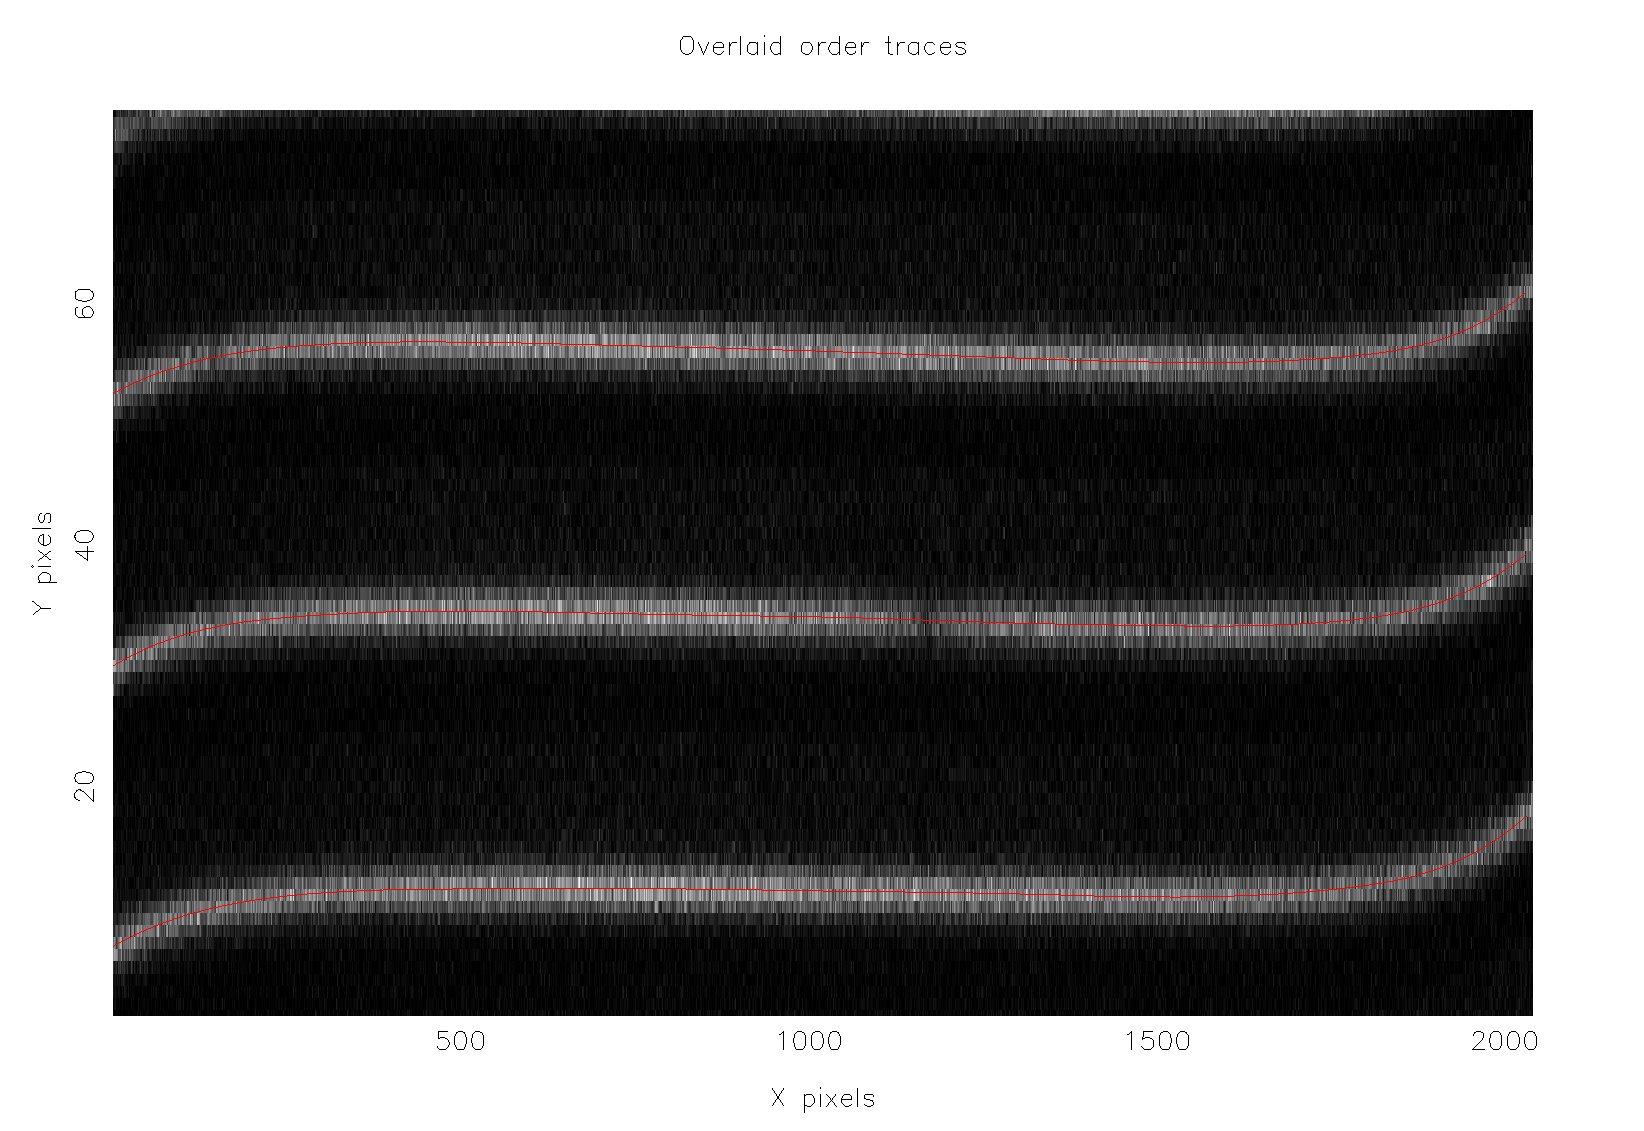
\includegraphics[width=\textwidth]{sun152_cover}

\parbox{140mm}{
\caption{A typical set of order paths as plotted using ECHMENU Option~15.
The distortions at the order extremities are due to the IPCS detector used.}
\label{fi_order2}
}
\end{center}
\end{figure}
\end{htmlonly}

Images not conforming to this format will need to be rotated through 90
degrees.

\subsection{\mlabel{CCD_bias_frames}CCD Bias Frames}
\myindex{CCD!bias}

A bias current is routinely applied to CCD detectors to ensure that, as
near as possible they are operating in a linear manner. This current
has the effect that a non-zero count is recorded in all pixels. The
observer should ensure that a number of `bias frames' are obtained to
adequately estimate the effect. The average of the bias frames should
be taken, and the result subtracted from all other frames before using
them in a reduction.  Failure to account for the bias may have a
detrimental effect on the signal-to-noise-ratio (S/N) in the final
spectrum.

{\sc echomop} does not provide any special facilities for the subtraction
of the bias current from CCD frames.  However, it does require that such
subtraction be performed {\bf before} processing takes place.
The bias subtraction may often be done automatically at the observatory
by the data recording software but it is up to you to check if this
is the case.
\xref{{\sc kappa}}{sun95}{CSUB} or \xref{{\sc figaro}}{sun86}{ICSUB} can be
used to subtract the bias if necessary.

For example:
\myindex{KAPPA!CSUB}
\myindex{FIGARO!ICSUB}
\begin{terminalv}
% csub /inframe/ /nnn/ /outframe/    (KAPPA)

% icsub /inframe/ /nnn/ /outframe/  (FIGARO)
\end{terminalv}

will subtract bias {\tt /nnn/} from data {\tt /inframe/} and put the
resulting data in {\tt /outframe/}\@.

For cases where the bias subtraction represents a significant source of
error it may be desirable to determine the error due to bias subtraction
on a pixel-by-pixel basis using many frames.
The resulting error estimates must then be copied into the object data
frames error arrays.
{\sc echomop} will incorporate these errors when calculating the
variances on the extracted spectra.

\subsection{\mlabel{CCD_overscan}CCD Overscan Region}
\myindex{CCD!overscan region}
\myindex{Bad row/column}
CCD frames typically include a number of rows/columns not exposed to the
light. The pixels in these rows often contain high counts and can affect
some of the automatic reduction procedures. It is prudent to clip off
these rows/columns before reduction proceeds. They will be the same for
all frames and can thus be removed using a simple looping command procedure.


\subsection{\mlabel{CCD_dark_count}CCD Dark Count}
\myindex{CCD!dark count}
Dark frames are essential for some applications. They are advisable when
using on-chip binning. For CCDs, the dark current may be high if it has
been exposed to too much light, or if power has been interrupted to a cold
chip. A number of long exposure (30 to 60 minutes) dark frames should be
combined using a median filter, and the result scaled according to the
object frame exposure time. This frame may then be subtracted from the
object frame before reduction begins. If you wish to ensure that the
error properties are accounted for then the dark frame should be copied
into the object frame variance array.

Again for CCDs only, a further advantage of collecting long exposure
dark frames is the option of deriving an independent estimate of the
rate of cosmic-ray events as a function of their intensity.  This can
provide a useful comparison with long exposure object frames and a check
on how effective cosmic-ray removal has been.

\subsection{\mlabel{flat_fielding}Flat Fielding}
\myindex{Flat field}
\myindex{Continuum lamp}
\myindex{Dekker}

A bright quartz lamp should be used with a dekker size a few steps
larger than that used for the object observations, but order overlapping
should of course be avoided. It is important to ensure that all orders
are as bright as possible. It may be necessary to use different
flat-field exposures to obtain good frames when observing in a spectral
region where the quartz lamp intensity or detector efficiency changes
rapidly. Each flat-field frame should be constructed by calculating the
median of a large number of runs where possible. If you wish to include
the errors on the flat-field then they should be placed in the flat-field
variance array.  If no variance estimates are provided then
root-N statistics will be assumed.\myindex{Variance}
{\sc echomop} can utilise different flat-field frames for different orders if
required.

\subsection{\mlabel{CCD_adu_to_photon}CCD Correction From Observed
            ADU to Photon Counts}
\myindex{ADUs}
\myindex{Photon counting statistics}
Many of the algorithms used assume that photon counting statistics
apply. However, it is unnecessary to correct raw frames since the
conversion factor (ADUs/photon) is prompted for when required.


\subsection{\mlabel{observer_arc_frames}Arc Frames}
\myindex{Arc lamp frames}
\myindex{UCLES}

In general arc frames should be obtained to bracket each object exposure
in time, allowing us to check that no shift has occurred during the
exposure. UCLES is extremely stable over relatively long periods and in
practice shifts are not detectable. The advantage of using a
single frame (possibly generated by co-adding the before and after arc
frames) is that this allows the resolution of the final spectrum to be
easily investigated. This is because the arc spectrum is always
extracted in an identical manner to that of the object; using the first
(and in this case only) supplied arc frame. As with the flat-field frame
it may also be advantageous to take multiple arc frames, each exposed
correctly to ensure high S/N in particular orders.  {\sc echomop} can
use a different arc frame for each order if required.

\subsection{\mlabel{frame_preparation}Preparing for a Reduction}
\myindex{Frame!preparation}

All raw data should be pre-processed in the following ways before
using {\sc echomop}:

\begin{itemize}

\item \myindex{ADAM!data files}
      The frames necessary for the reduction should be first converted into
      Starlink standard data files.  \xref{ADAM}{sg4}{} provides a set of
      tape reading and format translation utilities to help you do this.

\item \myindex{Frame!rotation}
      Rotate the data frame 90 deg.\ if necessary to achieve an orientation
      where the long axis of each order is in the X-pixel (horizontal)
      direction.

\item \myindex{CCD!bias}
      Subtract the BIAS current value from all raw frames using the
      \xref{{\sc kappa}}{sun95}{} \xref{CSUB}{sun95}{CSUB} command.

\item \myindex{ADUs}
      DO NOT multiply (CCD) frames by the prevailing ADU to electron
      conversion factor prior to reduction.  {\sc echomop} tasks prompt for
      this value and use it to generate resulting spectra with counts in
      photons.

\end{itemize}

\myindex{Cosmic rays}
If a cosmic-ray-contaminated frame is to be used for tracing the
paths of the orders across the frame then:

\begin{itemize}
\indexcmdname{ECH_DECOS1}
\indexcmdname{TUNE_CRTRC}

\item Use \htmlref{{\tt ech\_decos1}}{ech_decos1} to clean cosmic rays
      from the trace frame.
      This task flags cosmic rays in a quality array and does not actually
      alter any of the data frame values. This is the recommended approach
      in this situation. The \texttt{ech\_decos1} task may be used stand alone,
      or it may be invoked from the main task by specifying the
      parameters \htmlref{{\tt{TUNE\_CRTRC=YES}}}{par_TUNE_CRTRC} and
      \htmlref{{\tt{TUNE\_FCHECK=YES}}}{par_TUNE_FCHECK} at the
      start of a reduction.

\item If you have many `identical' object frames then these may be
      processed all together to provide a more reliable cosmic-ray
      rejection. The command procedure:

\begin{terminalv}
% $ECHOMOP_SOURCE/decos_many
\end{terminalv}

      \myindex{Exposure duration}
      provides this facility and should be the preferred method when
      multiple frames are available. The procedure calculates a median
      image and then rejects pixels which deviate by more than n sigma from
      the median value (note that this means that all the frames must be of
      equal exposure time). Bad pixels are flagged by placing values in the
      quality array of the frame concerned.

\end{itemize}


%%%%%%%%%%%%%%%%%%%%%%%%%%%%%%%%%%%%%%%%%%%%%%%%%%%%%%%%%%%%%%%%%%%%%%%%%%%
\newpage
\section{\mlabel{hints}PROBLEM HINTS}

\subsection{\mlabel{needs_rotating} Needs Rotating}
\myindex{Frame!rotation}

A data frame has been specified whose dimensions are orthogonal to those
of an already processed frame for this reduction. The most likely cause
is that one of the frames has been rotated and the other not. The
required frame geometry is to have the orders long axis aligned with the
horizontal (X-axis). The solution is to ensure that all
frames are consistent  and then re-start the reduction. In the case that
the first frame specified needs to be rotated then the reduction process
{\bf must} be re-started from the beginning using a new reduction file (delete
the current reduction file). In the case that that the first frame
specified was OK, then simply correcting the other frame and continuing
with the reduction will suffice.

\subsection{\mlabel{bad_x_dimension} Bad X Dimension}
\myindex{Frame dimensions}

A data frame has been specified whose X-dimension is different from that
of the first frame specified during the reduction. All frames {\bf must} have
the same X- and Y-dimensions. The most likely cause is that the frames
are from different datasets. If you really want to use this combination
of data frames then you must use the facilities of \xref{{\sc figaro}}{sun86}{}
to `grow' one
of the data frames up to the dimensions of the other.
Take care to ensure that any image registration problems are removed
before reduction is attempted.
In general it will be necessary to re-start the reduction with a new
reduction file after any such adjustments have been made.

\subsection{\mlabel{bad_y_dimension} Bad Y Dimension}

A data frame has been specified whose Y-dimension is different from that
of the first frame specified during the reduction. All frames {\bf must} have
the same X- and Y-dimensions. The most likely cause is that the frames
are from different datasets. If you really want to use this combination
of data frames then you must use the facilities of \xref{{\sc figaro}}{sun86}{}
to `grow' one
of the data frames up to the dimensions of the other.
Take care to ensure that any image registration problems are removed
before reduction is attempted.
In general it will be necessary to re-start the reduction with a new
reduction file after any such adjustments have been made.

\subsection{\mlabel{vmem_exhausted} Vmem Exhausted}
\myindex{Memory!running out}
\myindex{Running out of memory}

The program has run out of virtual memory space. The system command
`vmstat' produces a brief display of system memory status.
In particular, note the value which appears under the `free' column.
A low value here indicates that the whole system is running low,
otherwise it is likely that the problem is specific to your own
limits.  You may check these with the `limit' command.

\subsection{\mlabel{vmem_release} Vmem Release}

The program has been unable to release allocated memory correctly. The
most likely cause of this is attempting to continue processing after
having run out of virtual memory (Vmem\_exhausted). The only solution is
to abort the task and re-start.

\subsection{\mlabel{dimension_conflict} Dimension Conflict}

An attempt has been made to access a reduction object using dimensions
different from those operative at the time of its creation. This will
usually be due to the changing of a tuning (\texttt{TUNE\_???}) parameter
which is used to specify the dimension, or due to a change in wavelength
scale during scrunching (which changes dimensioning objects NX\_REBIN
and NO\_OF\_BINS). The name of the parameter is shown along with its
`old' and current value.

If a tuning parameter is involved then there are two courses of action
available. The first option is to reset the parameter to its previous
value and continue with the reduction. The second option is to delete
from the reduction file the object which has been created using the
`old' value. Such objects must then be re-created using the new
parameter value by invoking the relevant processing options. The program
will prompt as to which course of action is required. It should
be noted that in some cases deleting an object may necessitate the
re-running of an earlier option in order to re-create it, and
re-calculate its contents.
In this case you will be informed as to which step needs repeating.

\subsection{\mlabel{no_orders} No Orders}
\myindex{Locating orders!failure}

The task has been unable to find any orders in the frame supplied. The
most likely cause is that the frame has been incorrectly specified and
contains no orders. Another possibility is that the frame has the wrong
orientation (orders long axis horizontal) although at least one order
would usually be `found' in such a case. If the frame is correctly
specified and orientated then possible causes are as follows:

Cosmic-ray noise, use the \htmlref{{\tt ech\_decos1} task/ECHMENU Option~1.2}
{ech_decos1} to
clean the cosmic rays before re-trying order location.

Very poor S/N data, set the parameter
\htmlref{{\tt{TUNE\_AUTLOC=N}}}{par_TUNE_AUTLOC} to specify the
positions of the orders manually using a graphics cursor.

\subsection{\mlabel{bad_diagonals} Bad Diagonals}

The program is unable to determine the slope of the orders across the
frame. In this situation the slope is assumed to be 0. The most likely
cause is problems caused by cosmic-ray contamination which can be
avoided by using the \texttt{ech\_decos1} task/ECHMENU Option~1.2 to clean the
frame prior to slope determination.

The slope value is only used when tracing very poor data and it will not
usually cause problems if its value is left at zero.

In extreme cases you can set the slope manually using the
\xref{{\sc figaro}}{sun86}{} command \xref{SETOBJ}{sun86}{SETOBJ}:

\begin{terminalv}
% setobj object=-reduction-file-.MORE.ECHELLE.ORDER_SLOPE value=nn.nn
\end{terminalv}

where {\tt nn.nn} is the increase in y coordinate per X-pixel increment.

\subsection{\mlabel{wave_fit_start_end} Wave-fit Start/end}

The automated polynomial fit in wavelength has generated a wavelength
range which is inconsistent with the expected scope of wavelengths
(either as specified, or as calculated from previously identified orders).
You should investigate the identification of
this order manually to verify the situation.
In most cases allowing a larger search scope for the order and/or
manually rejecting the incorrect identification using the AI option in
\htmlref{{\tt ech\_idwave}}{ech_idwave} will
lead to a more favorable identification.

\subsection{\mlabel{wave_fit_deviations} Wave-fit Deviations}

The fitted polynomial has been rejected due to an excessive RMS
deviation measure. Usually the rejection will be valid and the program
will proceed to locate a better set of identifications. However, if
looking at the other orders shows that these
identifications are likely to be correct, then
\htmlref{{\tt ech\_idwave}}{ech_idwave}
should be used in its manual mode of operation. Specifying an
appropriate search range for the  order and using the AI option will let
the program relocate the set of identifications it rejected when running
automatically. You can then accept the set and interactively
improve it by adding/removing individual line identifications.

\subsection{\mlabel{cannot_create_db} Cannot Create DB}

The program is unable to create an arc line database file.
This is usually due to either the destination directory being
write-protected, or a disk quota being exceeded.

\subsection{\mlabel{feature_list_too_small} Feature List Too Small}

{\sc echomop} uses a special arc line information database to optimise its
search algorithm. This algorithm requires sets of approx. 12 lines with
which to work. The database consists of lines and their 10 nearest
neighbours on each side (l/r).  The arc-line list supplied (\texttt{.ARC} file)
does not contain sufficient lines for the database to be useful.
Either more lines must be added to the list,  or another program
(such as \xref{ECHARC}{sun86}{ECHARC}) must be used for the line
identification phase. It is
possible to add dummy entries to the line list just to overcome this
limitation, however in this case it is unlikely that automatic
identification will work and the program will probably need to be run
interactively.

\subsection{\mlabel{no_trace_width} No Trace Width}

The program failed to determine the width of the order traces. The
algorithm for this process requires that the intensity falls to less
than the fraction specified by \texttt{TUNE\_TWTHR} of the intensity at the
peak.  You may either adjust the parameter (probably increasing it),
or directly specify a value for the trace width using
\xref{{\sc figaro} SETOBJ}{sun86}{SETOBJ}:

\begin{terminalv}
 % setobj object=-rdctn-file-.MORE.ECHELLE.TRACE_WIDTH value=nn
\end{terminalv}

where {\tt nn} is the approximate width in pixels.


\subsection{\mlabel{corrupt_db} Corrupt DB}

A `read' operation on the arc line database has failed. The most likely
cause is that an inadvertent database creation has been performed which
has resulted in an incomplete copy of the database.  Check the database
files using

\begin{terminalv}
% ls -arc-list-type-.sdf
\end{terminalv}

and delete/rename any partial files.

\subsection{\mlabel{bad_sky_below} Bad Sky Below}
\myindex{Object limits!failure}

The program was unable to obtain a satisfactory estimate of the position
of the `sky' in the region below the object. The algorithm for
determining the sky extent uses the median intensity across the profile,
and the relative peak intensity. The relative peak intensity is
multiplied by the value of the parameter \texttt{TUNE\_SKYHILIM} and compared
with 1.05 times the median intensity. The lower of the two values is used as
a threshold. When the intensity falls below this threshold,  then the
program denotes the pixels from the current pixel to the edge of the
dekker as `sky'.  You may vary \texttt{TUNE\_SKYHILIM} to adjust the
threshold used. It is also possible to manually adjust the status of
each pixel in the profile by setting PFL\_INTERACT=Y.

\subsection{\mlabel{bad_sky_above} Bad Sky Above}

The program was unable to obtain a satisfactory estimate of the position
of the `sky' in the region above the object. The algorithm for
determining the sky extent uses the median intensity across the profile,
and the relative peak intensity. The relative peak intensity is
multiplied by the value of the parameter \texttt{TUNE\_SKYHILIM} and compared
with 1.05 times the median intensity. The lower of the two values is used as
a threshold. When the intensity falls below this threshold,  then the
program denotes the pixels from the current pixel to the edge of the
dekker as `sky'.  You may vary \texttt{TUNE\_SKYHILIM} to adjust the
threshold used. It is also possible to manually adjust the status of
each pixel in the profile by setting PFL\_INTERACT=Y.

\subsection{\mlabel{bad_lower_dekker} Bad Lower Dekker}
\myindex{Dekker limits!failure}

The program was unable to obtain a satisfactory estimate of the position
of the dekker in the region below the trace. The algorithm for
determining the dekker position steps out from the peak intensity until
the intensity falls below a tunable threshold. If the predicted edge is
reached before this occurs then the lower dekker is set to this
predicted value (simply calculated as half-way between the orders).

You may vary \texttt{TUNE\_DEKTHR} to adjust the threshold used.
It is also possible to manually adjust the status of each pixel in the
profile by setting \texttt{PFL\_INTERACT=Y}\@.

\subsection{\mlabel{bad_upper_dekker} Bad Upper Dekker}

The program was unable to obtain a satisfactory estimate of the position
of the dekker in the region above the trace. The algorithm for
determining the dekker position steps out from the peak intensity until
the intensity falls below a tunable threshold. If the predicted edge is
reached before this occurs then the lower dekker is set to this
predicted value (simply calculated as half-way between the orders).

You may vary \texttt{TUNE\_DEKTHR} to adjust the threshold used.
It is also possible to manually adjust the status of each pixel in the
profile by setting \texttt{PFL\_INTERACT=Y}\@.


\subsection{\mlabel{lost_left_trace} Lost Left Trace}
\myindex{Tracing order paths!failure}
\myindex{Order!tracing failure}

The program has failed to trace the order outwards from the centre of
the frame towards the left-hand side (decreasing X). If tracing is being
attempted using a cosmic-ray-contaminated frame then the
\htmlref{{\tt ech\_decos1} task/ECHMENU Option~1.2}{ech_decos1}
should be used to clean the frame prior to tracing.

The parameter \texttt{TUNE\_MXBADSMP} determines the number of failed
increments before the trace is `lost'.  The parameter \texttt{TUNE\_MXSMP}
determines the number of sampled increments across the frame and thus
their separation. In general increasing \texttt{TUNE\_MXSMP} will assist the
program in tracing difficult orders.  You should also experiment
with the various modes of tracing (controlled by \texttt{TRACE\_MODE} parameter)
which should allow most cases to be traced. As a last resort the program
also provides a manual trace mode in which points specified using a
graphics cursor (\xref{ICUR}{sun86}{ICUR} program) can be used as the basis
for the tracing process.


\subsection{\mlabel{lost_right_trace} Lost Right Trace}

The program has failed to trace the order outwards from the centre of
the frame towards the right-hand side (increasing X). If tracing is
being attempted using a cosmic-ray-contaminated frame then the
\htmlref{{\tt ech\_decos1} task/ECHMENU Option~1.2}{ech_decos1}
should be used to clean the frame prior to tracing.

The parameter \texttt{TUNE\_MXBADSMP} determines the number of failed
increments before the trace is `lost'. The parameter \texttt{TUNE\_MXSMP}
determines the number of sampled increments across the frame and thus
their separation. In general increasing \texttt{TUNE\_MXSMP} will assist the
program in tracing difficult orders.  You should also experiment
with the various modes of tracing (controlled by \texttt{TRACE\_MODE} parameter)
which should allow most cases to be traced. As a last resort the program
also provides a manual trace mode in which points specified using a
graphics cursor (\xref{ICUR}{sun86}{ICUR} program) can be used as the basis
for the tracing process.


\subsection{\mlabel{untraceable} Untraceable}

 The program could not trace the order at all.  Check that:

\begin{itemize}

\item the correct frame is being traced.

\item the frame is oriented so that the orders run with the dispersion
      direction parallel to the X-axis of the frame.

\end{itemize}

 If tracing has to be attempted using a cosmic-ray-con\-tami\-nated
 frame, try using the \htmlref{{\tt ech\_decos1} task/ECHMENU Option~1.2}
 {ech_decos1} to clean the frame prior to tracing.

 The parameter \texttt{TUNE\_MXSMP} determines the number of sampled increments
 across the frame and thus their separation.  In general, increasing
 \texttt{TUNE\_MXSMP} will assist the program in tracing difficult orders.
 It is worth experimenting with the various modes of tracing (set by
 the \texttt{TRACE\_MODE} parameter).  Usually, at least one of the available
 options will handle difficult or unusual cases.

 As a last resort a manual-trace mode, in which points specified using
 a graphics cursor (ICUR program) are used as the basis for the tracing
 process, is available.


\subsection{\mlabel{cannot_create_ech_rdctn} Cannot Create ECH\_RDCTN}
\myindex{Reduction database!cannot create}

The reduction database can not be created at this stage. You must
either use ECHMENU Option~1, or task \htmlref{{\tt ech\_locate}}{ech_locate},
as the first operation.
These ensure that the reduction database used by all
other task/operations is correctly created and initialised with the data
frame dimension information.

\subsection{\mlabel{cannot_create_ech_ftrdb} Cannot Create ECH\_FTRDB}

The specified file cannot be found and its automatic creation is illegal
using the selected option.

Please use the special task \texttt{ech\_ftrdb} to perform arc line database
creation. This process should normally be left to the node manager
who should place the database files in a commonly accessible
directory (usually the same place as the .ARC files). \myindex{Arc line
database creation} If you wish to create a private database for your
personally specified line list then use task \texttt{ech\_ftrdb} to do so. If
you are not trying to create a private database then the most likely
problem is that the environment-variable ARCDIRS has not been used to prefix
the arc database name ({\it{e.g.}}, ARCDIRS:THAR),
or that the named arc database does not exist (ask the system
manager).

If you wish to include a set of personally specified line list databases
in the default search paths used by {\sc echomop,} then their location should
be added to the list held in environment-variable ARCDIRS.  The list of
locations is searched in order of their appearance in the
environment-variable.  The default search path is:

\begin{quote}

   {\tt .} --- the current directory.

   {\tt ADAM\_USER} --- ADAM user directory.

   {\tt ECHOMOP\_EXEC } --- {\sc echomop} base directory.

\end{quote}

\subsection{\mlabel{not_a_reduction_format} Not a Reduction Format}

The specified file exists {\bf but} is not a reduction database as
defined by {\sc echomop} tasks. The most probable cause is that a data frame
file name has been provided by mistake.

The reduction database {\bf must} be created before the reduction
can start. The task
\htmlref{{\tt ech\_locate}/ ECHMENU Option~1}{ech_locate}
is currently the only one authorised to invoke reduction file creation so you
should use this if you need a new reduction database.

\subsection{\mlabel{no_update_access} No Update Access}

The program is unable to obtain update access to an array. This may be
either a DATA, QUALITY or ERROR array; and the most most probable cause
is that the file containing the array is protected against write access
in some way.  If the file is not owned by you, and in your directory,
then it is usually easiest to copy it into a directory to which you have
full access rights.


\subsection{\mlabel{cannot_create_here} Cannot Create Here}

The program is unable to create a reduction file as specified. The most
probable cause is due to the directory where the file creation is to be
performed being protected against write access, or does not exist at
all. Type:

\begin{terminalv}
% ls -l /name/of/directory
\end{terminalv}

to verify that the file exists, and to see what access rights the
current directory has.

If you own the directory in which file creation was attempted and have
the required access rights  then the most probable cause is the
exhaustion of system resources required, most notably disk space.
Type:

\begin{terminalv}
% quota
\end{terminalv}

to see if you have run out of space.


\subsection{\mlabel{no_cloneable_object} No Cloneable Object}
\myindex{Cloning!failure}

The program is unable to copy reduction database objects from the
specified reduction database.  The possible causes are that the
object in question does not exist in the reduction file specified
(either using \texttt{TUNE\_CLONE} or the \texttt{<} indirection operator in
ECHMENU), or that the object is dimensioned differently from the
corresponding object in the primary reduction database. Objects
can only be copied when their dimensionalities are identical ({\it{i.e.}} they
have the same number of X-pixels, number of orders {\it etc.}).

To check the dimensions of the object you are trying to clone from, use
the \xref{{\sc figaro}}{sun86}{} \xref{EXAM}{sun86}{EXAM} command and the object
path as reported by the program.  If the only dimensions which differ are
controlled by \texttt{TUNE\_} parameters,
then you may adjust the relevant parameter to allow the object
to be successfully copied (Note that this in turn may necessitate
re-running parts of the reduction to re-generate other objects also
dimensioned using the same \texttt{TUNE\_} parameter).

\subsection{\mlabel{read_only_rdctn_file} Read-Only RDCTN File}
\myindex{Reduction database!readonly}

The program is unable to obtain UPDATE access to an object in the
reduction database.  This is probably due to the file being
protected against write access. Type:

\begin{terminalv}
% ls -l /name/of/directory
\end{terminalv}

to check the file protection mask.

The program will continue {\bf but} please note that it will be unable to
write the results of the current step back into the reduction database.
You are therefore strongly recommended to copy the file to a location
where you have full access to it before proceeding.


%%%%%%%%%%%%%%%%%%%%%%%%%%%%%%%%%%%%%%%%%%%%%%%%%%%%%%%%%%%%%%%%%%%%%%%%%%%
\newpage
\section{\mlabel{release_notes}RELEASE NOTES}

\subsection{VERSION 3.3-0}

These notes formed a NEWS item at the time of release of version 3.3-0,
they describe the many changes from the previous, v3.2-0, release.

\subsubsection{Changes \& New Features}

\begin{itemize}
\item The parameter \htmlref{{\tt{ARC\_TYPE}}}{par_ARC_TYPE} is
   now ignored by the wavelength-calibration
   (Option 10) and wavelength-scale consistency checking (Option 20)
   tasks.  The parameter should be removed from any scripts which use
   these tasks before the next release of {\sc echomop,} at which point the
   parameter will be withdrawn.
\item The central order number and central wavelength of an
   echellogram can be used to constrain the automatic wavelength
   calibration process.  See parameter information for
   \htmlref{{\tt{CENTRAL\_ONUM}}}{par_CENTRAL_ONUM}
   and \htmlref{{\tt{CENTRAL\_WAVE}}}{par_CENTRAL_WAVE} for more details.
\item The output option (Option 14) can now produce DIPSO stacks of
   echelle data.  For example, to output a stack called
   \texttt{ECHOMOP\_STK.sdf} containing the extracted object orders:

\begin{terminalv}
% ech_result result_format=stack result_type=extobj stack=ECHOMOP
\end{terminalv}

   See the on-line HELP for more details.
\item When writing an ASCII file in Option 14 the name of the file can
   now be changed by setting the parameter
   \htmlref{{\tt{ASCII\_FILE}}}{par_ASCII_FILE}.
\item The Thorium-Argon arc-line list and database have been expanded.
\item A line list and database for Thorium-Neon arcs has been added.
   The relevant files are \texttt{THNE.ARC} and \texttt{THNE.sdf}.
\item An extra line has been added to the Copper-Argon line list and
   database.
\item Non-standard PGPLOT calls have been removed from the source code.
   This will lead to a minor performance improvement.
\item In the plotter, the ASCII-dump option now produces a files which
   DIPSO SP2RD can read.  The output filename is no longer fixed.
\item Deferred PGPLOT errors (which would be reported on exit from
   {\sc echomop}) have been removed.
\item The value \texttt{none} is now acceptable to indicate that no flat
   field (\htmlref{{\tt{FFIELD}}}{par_FFIELD} parameter) or no arc
   (\htmlref{{\tt{ARC}}}{par_ARC} parameter) is to  be used.
   Previously only the upper-case \texttt{NONE} could be used.  Note that
   only these two values indicate no available frame; a value of
   \texttt{None} or \texttt{NoNe} will be assumed to be the name of a frame.
\item In Option 1 (Locate orders) the criterion for detecting an order
   has been slightly changed.  Previously, a candidate order would
   have to have at least 1\% of the intensity of the brightest order
   found minus the median value of the central column in the image.
   This does not allow for automatic detection of all orders if the
   brightness of orders and the inter-order background level vary
   significantly across the frame.  The criterion has been changed
   to simply: `intensity at least 1\% of the brightest order'.
\item HELP is now available within the plotter task.
\end{itemize}

\subsubsection{Documentation notes}

\begin{itemize}
\item The database files used to store information about a specific
   reduction have been retitled `reduction databases'.  Previously
   these were known as `reduction structure files'.  This change is
   reflected in all documentation and source code comments.
\end{itemize}

\subsubsection{Fixes}

\begin{itemize}
\item When changing between arc-line databases there is no longer
   a prompt to choose between old and new values of
   \tt{TUNE\_WCAL\_INDEX}.
   This was a bug which would cause the program to crash if the user
   guessed `new' as the response to the prompt.
\item A memory management problem causing a crash if the abort `!'
   option was used in Options 3, 6, or 11 had been removed.
\item The parameter \htmlref{{\tt{CENTRAL\_ONUM}}}{par_CENTRAL_ONUM}
   can now be used, previously the
   value was forced to zero within the program.
\item In Option 4, the slit setup can now be edited.  Previously,
   each invocation of Option 4 would recalculate the settings.
   The settings can now be edited without this `reset' by setting
   \htmlref{{\tt{PFL\_MODE}}}{par_PFL_MODE} to the value \texttt{E}
   before starting the option.
\item The program now reports an error when unable to successfully
   access an input file.  The program reprompts the user.
   Previously the program would crash when trying to use `unaccessed'
   data.
\item The `Path syntax' in the plotter is now correctly displayed.
\item In browse mode in the plotter \texttt{SPLINE} traces are now supported.
   Previously \texttt{POLY} was assumed with unpredictable side-effects.
\item Limits in plotter browse mode are now correctly enforced, avoiding
   common crashes.
\item All advertised style options in the plotter now work.
\item A bug in Option 3 (Trace clip), which would decrease the number of
   knots for a \texttt{SPLINE} fit by 2 on each invocation, has been removed.
\item In Option 14 (Output results) the \texttt{OSPECT} output product can now
   be used without causing a crash.
\item The conversion from air to vacuum wavelengths enabled by
   \htmlref{{\tt{TUNE\_AIRTOVAC}}}{par_TUNE_AIRTOVAC} is applied to
   the output data file when requested.
   Previously, the correction was applied to the reduction database
   wavelengths, not to the output file.
\item A possible divide-by-zero error in Option 5 (Flat field) has been
   removed.
\item A missing range check in Option 9.2, which might give rise to
   segmentation faults, has been removed.
\end{itemize}

\subsection{VERSION 3.2-0}

These notes formed a NEWS item at the time of release of version 3.2-0, they
describe the many changes from the previous, v3.1-0, release.

{\bf General note:}
 Several modifications have been made to enhance the speed of the
 program.  Generally a reduction of about 35\% in execution time can
 be expected.

\subsubsection{New features}

\begin{itemize}
 \item A new task, \htmlref{{\tt{ech\_genflat}}}{ech_genflat},
   has been added.  This task outputs flat-field
   balance factors as generated by \htmlref{{\tt{ech\_ffield}}}{ech_ffield}
   to an image.  The image
   can then be inspected using, e.g., \xref{{\sc kappa}}{sun95}{}
   \xref{DISPLAY}{sun95}{DISPLAY}.
\item The design of the interface in parameter editors has been altered
   to make them a little easier to use.
\item The parameter \htmlref{{\tt{TUNE\_USE\_NXF}}}{par_TUNE_USE_NXF}
   has been `enhanced'.  Previously, this
   parameter set the fraction of an order (in the dispersion direction)
   to be used when profiling; setting the parameter to a value of 1.0
   selected a `special' mode where each order was separately profiled.
   This behaviour remains the same; however, it is now possible to
   select individual-order profiling and set the fraction of each order
   to be used.  For example, a value for {\tt TUNE\_USE\_NXF} of 1.2 selects
   the central 20\% of each order and individual-order profiling.
\item `QUIT' and `Q' have been added as aliases for EXIT in the \texttt{echmenu}
   top-level menu.
\item `Q' has been added as an alias for `E' (EXIT) in the
   \htmlref{{\tt{ech\_plot}}}{ech_plot} top-level menu.
\item The task \htmlref{{\tt{ech\_fcheck}}}{ech_fcheck} now checks both
   input and trace frames for
   bad-pixel values in their data arrays.  The trace frame is now
   checked for saturated pixels.
\item In the plotting task the full option menu is displayed only once.
   The menu can be redisplayed by pressing `M' as in other tasks.
\item In the plotting task when displaying reduction data the default
   prompt now automatically sets its self to point at the next order
   for the last data plotted.  For example a plot of `OBJ[1,1]' --- the
   first order of the object---will set the default value to `OBJ[1,2]'
   ---the next order.  This means it is much faster to check through all
   the orders.
\end{itemize}

\subsubsection{Documentation}

\begin{itemize}
\item ECHMENU option 1.5 has been documented in SUN/152.
\item Some errors in SUN/152 have been fixed, the text clarified in
   a few places, and several missing parameter details added.
\item Some errors in the on-line and hypertext HELP texts have been
   corrected.
\item The out-of-date and uninformative `Inputs-Outputs' and `Method'
   entries in the on-line and hypertext HELP text have been removed.
\end{itemize}

\subsubsection{Parameter default changes}

\begin{itemize}
\item The default value of \htmlref{{\tt{TUNE\_MXSMP}}}{par_TUNE_MXSMP}
   has been changed from 200 to 500.
   This reflects the increase in size of CCDs in recent years.
\item The advertised default value of
   \htmlref{{\tt{TUNE\_TWTHR}}}{par_TUNE_TWTHR} (0.9) was incorrect and
   has been corrected to 0.95.
\item The advertised default value of
   \htmlref{{\tt{TUNE\_AUTLOC}}}{par_TUNE_AUTLOC} (\texttt{YES}) was
   incorrect and has been changed to \texttt{NO}.
\item The advertised default value of
   \htmlref{{\tt{TRC\_NPOLY}}}{par_TRC_NPOLY}
   (7) was incorrect and has been changed to 4.
\item The default value of \htmlref{{\tt{TUNE\_ARCHIVE}}}{par_TUNE_ARCHIVE}
   has been changed to \texttt{NO}.
\item The default value of \htmlref{{\tt{MIN\_DISPERSION}}}{par_MIN_DISPERSION}
   has been changed to 0.01 which better reflects the dispersions used in
   \'{e}chelle instruments.
\end{itemize}

\subsubsection{Other changes}

\begin{itemize}
\item {\sc echomop} no longer uses the NAG library.
\item The module definition database has been removed.  Modules are defined
   as the program starts up.
\item Only one call to PSX\_UNAME is made per invocation of the monolith.
   Previously, several routines called PSX\_UNAME.
\item Calls to PGPOINT have been changed to call PGPT.
\item The subroutine calculating median values has been enhanced.
\item There is only one routine for mean/median/most-common-value
   calculation.
\item Several table look-up routines have been modified to exit-on-match,
   rather than searching the full table for an entry.
\item The trace-clipping task menu is only displayed once which speeds
   up the process of trace clipping.  The full menu can be displayed
   using option `M' in the same style as the profiling tasks.
\item In the spatial-profiling task the display of `below'-trace
   pixel-distances has been changed to reflect the syntax used.  For
   example the dekker edge is now said to be `20 pixels below trace'
   rather than `-20 pixels below' which suggests that it is above the
   trace.
\item Messages of the form `Parameter XXX is set to non-default value: nn'
   have been shortened.
\item Some of the main menu text has been changed.
\item Several (140) calls to ECH\_SET\_CONTEXT which had no effect have been
   removed from subroutines.  This may lead to a small speed-up for
   some operations.
\item When \htmlref{{\tt{DISPLAY=YES}}}{par_DISPLAY} overlaid trace plots are
   labelled with the relevant
   order number.  The display scaling is calculated per-order, which gives
   more satisfactory results.
\item The routine ECH\_FIND\_CENTRE has been modified, speeding up
   centre-of-gravity mode tracing and echmenu option 9 (locate arc line
   candidates).
\item The file ech\_dynamix\_index\_index.f (which was not used) has been
   removed.
\item The file ech\_makefits.f (which was not used and is not needed) has
   been removed.
\item The file ech\_plot\_id\_lines.f (which was not used) has been removed.
\item In the dekker/object-profiling task (echmenu option 4) graph titles
   now include the number of the order displayed.
\item Many FORMAT statements have been changed by the addition of `1P'
   scale factors.  This makes output numbers easier to read.
\item The files ech\_loop\_nvariable.f and ech\_loop\_variable.f have been
   removed due to the process of speeding up the main {\sc echomop} routine
   and introduction of extra functions.
\item The IDX\_ parameters were being typed as \_REAL by the program whilst
   they were (correctly) declared as \_INTEGER in interface files.
   This has been corrected.
\item In the order-blaze fitter the plots of function-verses-fit now
   use the same colour scheme as in the order trace fitter.
\item The displays and menus in the interactive flat-field modeller have
   all been tidied up.
\item In the trace-clipping task the `.'\ option now deletes the nearest
   point to the cursor as advertised.  Previously this deleted the
   nearest point in X.  This change also affects the blaze-fitter and
   sky-modeller.
\item ECH\_FATAL\_ERROR and ECH\_CALC\_TRACE have been modified to speed up
   the program.
\end{itemize}

\subsubsection{Fixes}

\begin{itemize}
\item In the order-fitting/clipping process it is now possible to
   select an order of fit less than 4.
\item In the {\tt ech\_spatial} task it is no longer possible to set the
   value of DEK\_BELOW greater than DEK\_ABOVE and vice versa.
   Previously this would cause various problems.
\item Internal arrays in profiling tasks have been enlarged and
   range checks are now performed prior to array usage.  This
   has removed some intermittent crashes.
\item Most FORMAT statements using Hollerith characters have been updated.
\item An error in the data access layer relating to default object
   dimensions has been fixed.
\item Previously, in plots of order-trace versus fitted-curve the points
   of the order trace were shifted down.  This gave the impression that
   the fit was offset by a constant.  This bug has been removed.
   This bug also affected the order trace overlaid on image plots.
\item A limitation in ECH\_MEAN\_MEDIAN whereby only the first 5000 values of
   a dataset would be used in median determination has been removed.
\item An error causing a crash for
   \htmlref{{\tt{USE\_MEDIAN=YES}}}{par_USE_MEDIAN} in the order-location
   task has been removed.  {\tt USE\_MEDIAN=YES} now works OK.
\item An error in the call sequence causing unaligned memory access and
   crashing {\tt ECH\_DECOS2} has been removed.
\item Spurious `Unknown fitting function' messages appearing when using
   {\tt ECH\_DECOS2} have been removed.
\item Centroid-mode tracing now includes a filter for bad values in images.
   Previously, these bad values would break the centroiding code causing
   a crash with a floating-point exception.
\item The spatial-profiling task now includes various filters for bad
   values which would break it.
\item A commonly-occurring divide-by-zero error in the optimal extraction
   algorithm implementation has been removed.
\item The simple extraction algorithm will now handle bad-pixel values as
   well as, or instead of, quality arrays in object images.
\item The simple extraction algorithm will now handle bad-pixel values in
   arc images.
\item The profile-weighted extraction algorithm will now handle bad-pixel
   values as well as, or instead of, quality arrays in object images.
\item The profile-weighted extraction algorithm will now handle bad-pixel
   values in arc images.
\item The HELP facility is now accessible from the echmenu program (bug in
   v3.1-0).
\item The quick-look extraction algorithm will now handle bad-pixel
   values as well as, or instead of, quality arrays in object images.
\item The quick-look extraction algorithm will now handle bad-pixel
   values in arc images.
\item After running the quick-look extraction the colour of plots is now
   reset to black rather than being left blue.
\item The 2-D simple-extraction algorithm will now handle bad-pixel values
   in arc images.
\item The 2-D simple-extraction algorithm will now handle bad-pixel values
   as well as, or instead of, quality arrays in object images.
\item The arc-line width estimator routine can now handle bad values in the
   image.  The routine has been improved to scale data according to the
   number of good values obtained, previously no scaling was applied.
\item After running the trace-consistency checker the colour of plots is
   now reset to black rather than being left red.
\item The blaze-fitting option now checks for the case
   \htmlref{{\tt{TUNE\_NOFLAT=YES}}}{par_TUNE_NOFLAT},
   previously it would simply crash in this case.
\item After running the order-trace plotting task the colour of plots is
   now reset to black rather than being left red.
\item Image displays autoscale to suit the data rather than using fixed
   (incorrect) values dependant on the image dimensions.
\item Order tracing with \htmlref{{\tt{DISPLAY=YES}}}{par_DISPLAY} now works,
   previously this caused
   a crash due to a type mismatch in a subroutine call.
\item Previously, order tracing with fitted traces displayed overlaid on
   the traced image only worked when some other plot had been made in
   the session.  This can now be the first plot in a session.
\item A crash when running the trace-consistency checker with
   {\tt DISPLAY=YES} has been removed.
\item Evaluation of SPLINE-fitted order traces in the order-tracing task
   was not done correctly, causing the program to crash in some cases.
   This bug has been removed.
\item Reporting of messages relating to NULL (!) and ABORT (!!) responses
   to parameter prompts is no longer deferred.
\item The faulty arc-line database file \texttt{\$ARCDIRS/THAR.sdf}
   has been replaced.
\item Incomplete database entries in \texttt{\$ARCDIRS/} \texttt{THAR.sdf} and
   \texttt{CUAR.sdf}
   have been filled.  The first 10 and last 11 entries, which should be
   partially present, were completely omitted.  The database builder has
   been corrected to add the partial entries.
\item When using {\tt ech\_idwave}, in the case of one identified feature in an
   order, the program would crash when trying to determine the wavelength
   range for the order.  This bug has been removed.
\item Option `M' in the {\tt ech\_idwave} task, order-processing menu,
   no longer crashes the program.
\item In the {\tt ech\_idwave} task, in the event of a wavelength polynomial
   being
   of such a low-order that all points are fitted exactly (giving zero
   RMS error) the program no longer crashes on a divide-by-zero.
\item The interactive mode of {\tt ech\_idwave}, options \texttt{<} and \texttt{>}
   no-longer cause a crash when the display is not zoomed.
\item In the interactive mode of {\tt ech\_idwave}, option `I' would work only
   once per option `P' this has been fixed.
\item In the interactive mode of {\tt ech\_idwave}, option `I', the list of
   nearby
   features is centred on the selected feature, rather than the next
   feature up in wavelength.
\item Arc line database files no longer have to have write access enabled.
   This means that files in \texttt{\$ARCDIRS} do not have to be copied to an
   {\sc echomop} user's working directory.
\item Several missing parameters have been added to the interface files.
\item An infinite loop on detection of bad columns or rows in {\tt ech\_fcheck}
   has been removed.
\item A divide-by-zero error in {\tt ech\_ffield} for local mean or median
   calculation has been removed.
\item In {\tt ech\_ffield} the calculation of local medians now uses the correct
   start point in the X-direction.  Previously, the median for the start
   point X\sunspec{$-$}{-}{\tt{TUNE\_FFLSMP}} rather than
   X\sunspec{$-$}{-}({\tt{TUNE\_PFLSMP}}/2), was being used.
\item In {\tt ech\_fitblz}, a floating point overflow could occur when automatic
   fitting became unstable.  The overflows are now clipped.
\item The type of the parameter
   \htmlref{{\tt{TUNE\_SCFRACT}}}{par_TUNE_SCFRACT} was incorrectly set as
   \_INTEGER.  It is now \_REAL.
\item Several internal changes to the scrunching routines have been made to
   prevent scrunched spectra being reflected in the wavelength axis,
   {\it{i.e.}}, all the fluxes being negative.
\item Errors in the sky modeller which would lead to attempted processing
   of points outside the bounds of an image have been removed.
\item The sky modeller now filters out bad-pixel values.
\item The object profile modeller now filters out bad-pixel values.
\item In several tasks, notably the extractions, weighting of the
   contribution from `boundary' pixels has been corrected to a smooth
   function.  The function previously had two discontinuities at the top
   and bottom edges of the extraction channel---introducing a `jump' in
   some data.
\item Errors in the pixel-weighting scheme implementation and pixel
   selection in the blaze fitter have been removed.
\item ECHMENU Option 1.2 ({\tt{ech\_decos1}}) is now allowed to be an automated
   step. Previously the value of \htmlref{{\tt{TUNE\_CRTRC}}}{par_TUNE_CRTRC}
   was always taken as \texttt{NO} in
   this case.  In the same way, Options 11.3 and 11.4 now also work as
   elements in a {\tt TUNE\_AUTOMATE} request.
\item NDF\_SQMF has been used to switch off automatic QUALITY component
   checking as {\sc echomop} does this itself.
\item The copy-last-plot-to-hardcopy device option in {\tt ech\_plotter}
   now works.
\item Several divide-by-zero opportunities in the 2-D sky modeller have been
   removed.
\item The 2-D sky modeller now handles bad-pixel values in input data.
\item The routine which identifies order numbers now works, this helps
   automatic wavelength calibration proceed faster.
\end{itemize}


%%%%%%%%%%%%%%%%%%%%%%%%%%%%%%%%%%%%%%%%%%%%%%%%%%%%%%%%%%%%%%%%%%%%%%%%%%%

% We could include the sun152.ind file here with \printindex (requires
% \usepackage{makeidx} at the top), but instead we paste the generated
% index in in place.
\begin{theindex}

  \item 2-D distortion, 37
    \subitem viewing, 82
  \item \cmdname {2D_INTERACT}, 77

  \indexspace

  \item Abort
    \subitem option, 5
  \item Accept character, 3
  \item ADAM
    \subitem data files, 90
    \subitem from spawned process, 50
    \subitem parameters, 5
  \item ADUs, 89, 90
  \item All order processing, 46
  \item \cmdname {ARC}, 51
  \item Arc calibration
    \subitem none, 8
  \item Arc fitting
    \subitem blends, 30
    \subitem clear, 31
    \subitem delete line, 31
    \subitem hardcopies, 32
    \subitem list known lines, 31
    \subitem new line, 31
    \subitem set wavelength, 32
  \item Arc frames, 82
    \subitem multiple, 85
  \item Arc lamp frames, 90
  \item Arc line
    \subitem calibration, 7, 29
    \subitem FWHM, 7, 28
    \subitem FWHM fit, 7
    \subitem location, 7, 27
  \item Arc line database creation, 96
  \item Arc line lists
    \subitem format, 84
  \item \cmdname {ARC_TYPE}, 52
  \item \cmdname {ASCII_FILE}, 52
  \item \cmdname {AUTO}, 52
  \item \cmdname {AUTO_ID}, 52
  \item Automation, 8, 77
    \subitem functions, 8
    \subitem requirements, 8

  \indexspace

  \item Bad row/column, 10, 89
  \item \cmdname {BAD_ORDER}, 52
  \item Batch processing, 78
  \item \cmdname {BIN_SIZE}, 52
  \item Blaze, 82
  \item \cmdname {BLZ_INTERACT}, 53
  \item \cmdname {BLZ_NPOLY}, 53
  \item \cmdname {BLZFIT}, 52

  \indexspace

  \item CCD, 80
    \subitem bias, 88, 90
    \subitem dark count, 89
    \subitem overscan region, 89
  \item \cmdname {CENTRAL_ONUM}, 53
  \item \cmdname {CENTRAL_WAVE}, 53
  \item Cloning, 78
    \subitem failure, 97
  \item Closedown, 51
  \item Continuum lamp, 89
  \item Copy line identifications, 79
  \item Cosmic rays, 7, 11, 90
    \subitem coincidence checking, 42, 81
    \subitem imaging, 42
    \subitem location of, 80
    \subitem order location, 11
    \subitem post-trace location, 41
    \subitem using Horne algorithm, 26
    \subitem when to locate, 21
  \item \cmdname {CR_OUTPUT}, 53

  \indexspace

  \item Data frames, 84
  \item Data quality, 42
  \item \cmdname {DECIMG}, 53
  \item Dekker, 89
  \item Dekker limits, 7, 19
    \subitem failure, 94
  \item Delete order, 47
  \item Demonstration, 2, 8
  \item Disable order, 47
  \item Disk space
    \subitem running out, 84
  \item \cmdname {DISPLAY}, 53

  \indexspace

  \item \cmdname {ECH_ALL}, 46
  \item \cmdname {ECH_BLAZE}, 34
  \item \cmdname {ECH_COUNT}, 11
  \item \cmdname {ECH_DECIMG}, 42
  \item \cmdname {ECH_DECOS1}, 90
  \item \cmdname {ECH_DECOS2}, 41
  \item \cmdname {ECH_DISABLE}, 47
  \item \cmdname {ECH_ECHAR}, 54
  \item \cmdname {ECH_EXIT}, 51
  \item \cmdname {ECH_EXT2D}, 37
  \item \cmdname {ECH_EXTRCT}, 26
  \item \cmdname {ECH_FFIELD}, 22
  \item \cmdname {ECH_FITORD}, 15
  \item \cmdname {ECH_FTRDB}, 54
  \item \cmdname {ECH_GENFLAT}, 50
  \item \cmdname {ECH_IDWAVE}, 29, 79
  \item \cmdname {ECH_LINLOC}, 27
  \item \cmdname {ECH_LOCATE}, 10
  \item \cmdname {ECH_MDLBCK}, 45, 82
  \item \cmdname {ECH_MENU}, 50
  \item \cmdname {ECH_MULMRG}, 44
  \item \cmdname {ECH_PLOT}, 47, 83
  \item \cmdname {ECH_PROFILE}, 25
  \item \cmdname {ECH_QEXTR}, 43
  \item \cmdname {ECH_RDCTN}, 54
  \item \cmdname {ECH_RDUCD}, 54
  \item \cmdname {ECH_RESULT}, 39
  \item \cmdname {ECH_SCRN2D}, 82
  \item \cmdname {ECH_SCRUNCH}, 35
  \item \cmdname {ECH_SINGLE}, 46
  \item \cmdname {ECH_SKY}, 24
  \item \cmdname {ECH_SPATIAL}, 19, 24, 80
  \item \cmdname {ECH_STRUCT}, 54
  \item \cmdname {ECH_SYSTEM}, 50
  \item \cmdname {ECH_TRACE}, 13
  \item \cmdname {ECH_TRCSIS}, 40
  \item \cmdname {ECH_TRPLT}, 15, 40
  \item \cmdname {ECH_TUNER}, 5, 46
  \item \cmdname {ECH_WVCSIS}, 43
  \item \cmdname {ECHARC} data exchange, 30
  \item \cmdname {ECHHELP}, 10
  \item Errors
    \subitem additive, 9
    \subitem arrays, 9
    \subitem due to cosmic rays, 9
    \subitem multiplicative, 9
    \subitem on flat field, 23
    \subitem output, 9
    \subitem Sky model, 9
  \item Exit, 51
  \item Exposure duration, 90
  \item Extended object frames, 80
  \item \cmdname {EXTRACT_MODE}, 54
  \item Extraction, 7, 26
    \subitem quick-look, 8, 26, 43
  \item Extraction limits, 7

  \indexspace

  \item \cmdname {FFIELD}, 54
  \item Fibre-fed spectrographs, 79
  \item FIGARO
    \subitem ECHARC, 87
    \subitem ICSUB, 88
    \subitem IMAGE, 47
    \subitem SCRUNCH, 36
    \subitem SETOBJ command, 11
    \subitem SOFT, 4
  \item \cmdname {FLAG}, 55
  \item Flat field, 7, 22, 89
    \subitem defines dekker, 19
    \subitem errors, 9
    \subitem none, 23
  \item \cmdname {FLTFIT}, 23, 55
  \item Flux calibration, 81
    \subitem frames, 86
  \item Flux standards, 81
  \item Frame
    \subitem dimensions, 7, 10
    \subitem preparation, 90
    \subitem rotation, 88, 90, 91
  \item Frame dimensions, 91
  \item \cmdname {FRAME_CHECK}, 55

  \indexspace

  \item Graphics
    \subitem hardcopy, 4
    \subitem multiple per screen, 49
    \subitem null device, 4
    \subitem plot utility, 47
    \subitem setting device, 4

  \indexspace

  \item \cmdname {HARD}, 55
  \item \cmdname {HELIO_COR}, 55
  \item Heliocentric correction, 83
  \item Help, 4, 10
  \item \cmdname {HI_WAVE}, 55
  \item Hidden parameters
    \subitem edit, 46

  \indexspace

  \item \cmdname {ID_INTERACTIVE}, 56
  \item \cmdname {IDX_NREF_FRAME}, 55
  \item \cmdname {IDX_NUM_ORDERS}, 55
  \item Ignore order, 47
  \item Image display, 5
    \subitem use by monolith, 5
  \item \cmdname {INDIRECT}, 56
  \item \cmdname {INPTIM}, 56
  \item Input data files, 83
  \item IPCS, 80

  \indexspace

  \item KAPPA
    \subitem CSUB, 88

  \indexspace

  \item Locating orders, 7, 11
    \subitem failure, 92
  \item Longslit spectra, 79
  \item \cmdname {LOW_WAVE}, 56

  \indexspace

  \item Main menu
    \subitem monolith, 10
  \item Manual dekker limits, 21
  \item Manual object limits, 21
  \item Manually set order path, 14
  \item Masks
    \subitem sky/object, 19
  \item \cmdname {MAX_DISPERSION}, 56
  \item Memory
    \subitem running out, 91
  \item Merge multiple spectra, 36, 44
  \item \cmdname {MIN_DISPERSION}, 56
  \item Monolith, 3
  \item Multi-object frames, 79
  \item Multiple data frames, 6
  \item Multiple object frames, 8, 36, 44, 81, 86

  \indexspace

  \item \cmdname {NREF_FRAME}, 57
  \item \cmdname {NUM_ORDERS}, 57

  \indexspace

  \item \cmdname {OBJ_SKY_GAP}, 57
  \item Object
    \subitem profile, 7
  \item Object frames
    \subitem multiple, 86
  \item Object limits, 7, 19
    \subitem failure, 94
  \item Object profile, 25
  \item \cmdname {OBJFIT}, 57
  \item Observing Hints, 88
  \item Option
    \subitem abort, 5
    \subitem selection of, 3
  \item Order
    \subitem blaze, 34
    \subitem disabling, 16
    \subitem location, 7, 11
    \subitem process single, 46
    \subitem ripple, 7
    \subitem slope, 7, 11
    \subitem trace optimisation, 15
    \subitem trace plotting, 40
    \subitem traces consistency check, 40
    \subitem tracing, 7, 13
    \subitem tracing failure, 95
    \subitem viewing traces, 15
  \item Orientation of frames, 29
  \item Orientation of spectra, 88
  \item Output, 8, 39
  \item Output files, 86
  \item \cmdname {OUTPUT_IMAGE}, 57
  \item Overlaying graphs, 49

  \indexspace

  \item Parameters, 5
    \subitem edit tuning, 46
    \subitem hidden, 5
    \subitem tuning, 5
  \item Partial orders, 13
  \item \cmdname {PFL_INTERACT}, 21, 57
  \item \cmdname {PFL_MODE}, 57
  \item Photon counting statistics, 89
  \item \cmdname {PHOTON_TO_ADU}, 58
  \item Pixel response variations, 22
  \item Plot styles, 49
  \item Plotter, 47
    \subitem image browse, 47
    \subitem known objects, 48
    \subitem overlaying, 49
    \subitem rebinning, 49
    \subitem set limits, 48
    \subitem subsets, 48
  \item Profile
    \subitem object, 7
  \item Prompt, 4
    \subitem disabling, 5

  \indexspace

  \item Quality array, 42
  \item Quick-look extraction, 8, 26, 43
  \item Quick-look mode, 9

  \indexspace

  \item \cmdname {RBNOBJ}, 58
  \item Re-binning
    \subitem 2-D, 38
    \subitem using plotter, 49
  \item Readout noise, 9, 81
  \item \cmdname {READOUT_NOISE}, 58
  \item Reduction database, 3, 83
    \subitem cannot create, 96
    \subitem cloning, 78
    \subitem readonly, 97
  \item Repeating steps, 6
  \item \cmdname {RESULT_FORMAT}, 58
  \item \cmdname {RESULT_TYPE}, 58
  \item Results, 8
    \subitem output of, 39
  \item Ripple, 82
  \item Ripple correction, 34
  \item Running out of memory, 91

  \indexspace

  \item Saturated pixels, 10
  \item Saving results, 86
  \item Scattered light, 82
  \item Scrunch
    \subitem arc, 7
    \subitem object, 7
  \item \cmdname {SCRUNCH_TYPE}, 58
  \item Scrunching, 35
  \item \cmdname {SET_WSCALE}, 59
  \item Signal-to-noise, optimal extraction, 26
  \item Single step tasks, 6
  \item Sky
    \subitem errors, 9
    \subitem model, 7
    \subitem noise simulation, 24
    \subitem subtraction, 24
  \item Sky lines, 81
  \item \cmdname {SKYFIT}, 59
  \item \cmdname {SLITIM}, 59
  \item Slope of orders, 7
  \item \cmdname {SOFT}, 59
  \item Spatial profile, 25
  \item Spatial subsampling, 25
  \item Spatially resolved spectra, 19
  \item Spawning a subprocess, 50
  \item \cmdname {STACK}, 59
  \item Standard reduction
    \subitem sequence, 10
  \item Standard stars, 81
  \item \cmdname {START_WAVE}, 59
  \item Starting a reduction, 10
  \item Starting up, 3
  \item Structure definition files, 85
  \item Sub-options, 8
    \subitem selection of, 4
  \item System commands, 50

  \indexspace

  \item Trace
    \subitem consistency, 14, 40
    \subitem frame, 88
    \subitem order paths, 13
    \subitem orders, 7
  \item \cmdname {TRACE_MODE}, 59
  \item \cmdname {TRACIM}, 60
  \item Tracing, 88
  \item Tracing order paths
    \subitem failure, 95
  \item \cmdname {TRC_INTERACT}, 60
  \item \cmdname {TRC_NPOLY}, 61
  \item \cmdname {TRC_VETO}, 61
  \item \cmdname {TRCFIT}, 60
  \item Trouble-shooting, 83
  \item \cmdname {TUNE_AAACODE}, 61
  \item \cmdname {TUNE_AIRTOVAC}, 61
  \item \cmdname {TUNE_ARCHIVE}, 62
  \item \cmdname {TUNE_AUTLOC}, 11, 62, 77
  \item \cmdname {TUNE_AUTOID}, 78
  \item \cmdname {TUNE_AUTOMATE}, 62, 78
  \item \cmdname {TUNE_BATCH}, 62, 77
  \item \cmdname {TUNE_BLZRSET}, 34, 62
  \item \cmdname {TUNE_CLONE}, 62
  \item \cmdname {TUNE_CLPBY}, 63
  \item \cmdname {TUNE_CLPMXDEV}, 63
  \item \cmdname {TUNE_CNSDEV}, 40, 63
  \item \cmdname {TUNE_CRCLEAN}, 26, 63
  \item \cmdname {TUNE_CRINTER}, 63
  \item \cmdname {TUNE_CRMAX}, 63
  \item \cmdname {TUNE_CRTRC}, 11, 64, 77, 90
  \item \cmdname {TUNE_CRXBOX}, 64
  \item \cmdname {TUNE_CRYBOX}, 64
  \item \cmdname {TUNE_DB_SCOPE}, 64
  \item \cmdname {TUNE_DEKABV}, 64
  \item \cmdname {TUNE_DEKBLW}, 64
  \item \cmdname {TUNE_DEKTHR}, 64
  \item \cmdname {TUNE_DIAGNOSE}, 64
  \item \cmdname {TUNE_DPRBTHR}, 65
  \item \cmdname {TUNE_DSGMTHR}, 65
  \item \cmdname {TUNE_FCHECK}, 10, 11, 65, 77
  \item \cmdname {TUNE_FFINTER}, 65
  \item \cmdname {TUNE_FFLMED}, 65
  \item \cmdname {TUNE_FFLSMP}, 65
  \item \cmdname {TUNE_FFNXPLY}, 66
  \item \cmdname {TUNE_FFNXREJ}, 66
  \item \cmdname {TUNE_FFNYPLY}, 66
  \item \cmdname {TUNE_FFNYREJ}, 66
  \item \cmdname {TUNE_FFSUBSMP}, 66
  \item \cmdname {TUNE_FFTHRESH}, 66
  \item \cmdname {TUNE_FIBRES}, 67
  \item \cmdname {TUNE_FINCPLY}, 67
  \item \cmdname {TUNE_FLUX}, 67
  \item \cmdname {TUNE_HELIO}, 67
  \item \cmdname {TUNE_IDINMN}, 67
  \item \cmdname {TUNE_IDINMX}, 67
  \item \cmdname {TUNE_IDMDLT}, 67
  \item \cmdname {TUNE_IDMXDIF}, 67
  \item \cmdname {TUNE_IDSDLT}, 68
  \item \cmdname {TUNE_IDSTRNG}, 68
  \item \cmdname {TUNE_INTR}, 68
  \item \cmdname {TUNE_IUE}, 68
  \item \cmdname {TUNE_LOG}, 68
  \item \cmdname {TUNE_MAX2DPLY}, 68
  \item \cmdname {TUNE_MAX2DPNTS}, 68
  \item \cmdname {TUNE_MAXLINES}, 68
  \item \cmdname {TUNE_MAXPOLY}, 68
  \item \cmdname {TUNE_MAXRFLN}, 69
  \item \cmdname {TUNE_MERGE}, 69
  \item \cmdname {TUNE_MINCR}, 69
  \item \cmdname {TUNE_MRGMAXX}, 69
  \item \cmdname {TUNE_MRGMINX}, 69
  \item \cmdname {TUNE_MRGWGHT}, 44, 69
  \item \cmdname {TUNE_MXBADSMP}, 69
  \item \cmdname {TUNE_MXSKYPIX}, 69
  \item \cmdname {TUNE_MXSMP}, 69
  \item \cmdname {TUNE_NOARC}, 70
  \item \cmdname {TUNE_NOFLAT}, 23, 70
  \item \cmdname {TUNE_OBJABV}, 70
  \item \cmdname {TUNE_OBJBLW}, 70
  \item \cmdname {TUNE_OBJPOLY}, 25, 70
  \item \cmdname {TUNE_OBJREJ}, 70
  \item \cmdname {TUNE_OBJRTHR}, 71
  \item \cmdname {TUNE_PAGE}, 71
  \item \cmdname {TUNE_PARTORD}, 71
  \item \cmdname {TUNE_PFLSSAMP}, 25, 71
  \item \cmdname {TUNE_PFSAMP}, 71
  \item \cmdname {TUNE_PREBAL}, 23, 71
  \item \cmdname {TUNE_QUAD}, 72
  \item \cmdname {TUNE_QUICK}, 9, 72
  \item \cmdname {TUNE_REPORT}, 72
  \item \cmdname {TUNE_REVCHK}, 29, 72
  \item \cmdname {TUNE_RFLNTHR}, 72
  \item \cmdname {TUNE_SATRTN}, 10, 73
  \item \cmdname {TUNE_SCFRACT}, 73, 82
  \item \cmdname {TUNE_SCRADD}, 73
  \item \cmdname {TUNE_SCRMODE}, 73
  \item \cmdname {TUNE_SKEW}, 73
  \item \cmdname {TUNE_SKVRCORR}, 73
  \item \cmdname {TUNE_SKYHILIM}, 74
  \item \cmdname {TUNE_SKYINTER}, 74
  \item \cmdname {TUNE_SKYLINW}, 24, 74
  \item \cmdname {TUNE_SKYLTHR}, 24, 74
  \item \cmdname {TUNE_SKYPOLY}, 74
  \item \cmdname {TUNE_SKYREJ}, 75
  \item \cmdname {TUNE_SKYRTHR}, 75
  \item \cmdname {TUNE_SKYSIM}, 24, 75
  \item \cmdname {TUNE_SKYXPLY}, 75
  \item \cmdname {TUNE_TRCNS}, 40, 75
  \item \cmdname {TUNE_TWTHR}, 75
  \item \cmdname {TUNE_UHRF}, 76
  \item \cmdname {TUNE_USE_NXF}, 19, 25, 76
  \item \cmdname {TUNE_USEAAA}, 76
  \item \cmdname {TUNE_XBOX}, 76
  \item \cmdname {TUNE_XZONE}, 76
  \item \cmdname {TUNE_YBLAZE}, 76
  \item \cmdname {TUNE_YZONE}, 77
  \item Tuning parameters
    \subitem edit, 46

  \indexspace

  \item UCLES, 90
  \item \cmdname {USE_MEDIAN}, 77
  \item User-calculated balance factors, 23
  \item Using data from previous reduction, 78

  \indexspace

  \item Variance, 9, 89
  \item Viewing spectra, 83

  \indexspace

  \item \cmdname {W2_NX_POLY}, 77
  \item \cmdname {W2_NY_POLY}, 77
  \item \cmdname {W_NPOLY}, 77
  \item Wavelength calibration, 7, 29
    \subitem fibre data, 79
    \subitem none, 8
  \item Wavelength scales
    \subitem 2-D, 38
    \subitem cloning, 78
    \subitem consistency check, 43
    \subitem reversed, 29
  \item \cmdname {WAVFIT}, 77
  \item Weighting
    \subitem during co-addition, 36
    \subitem during extraction, 26

\end{theindex}


% ? End of main text
\end{document}
